
% Default to the notebook output style

    


% Inherit from the specified cell style.




    
\documentclass[11pt]{article}

    
    
    \usepackage[T1]{fontenc}
    % Nicer default font (+ math font) than Computer Modern for most use cases
    \usepackage{mathpazo}

    % Basic figure setup, for now with no caption control since it's done
    % automatically by Pandoc (which extracts ![](path) syntax from Markdown).
    \usepackage{graphicx}
    % We will generate all images so they have a width \maxwidth. This means
    % that they will get their normal width if they fit onto the page, but
    % are scaled down if they would overflow the margins.
    \makeatletter
    \def\maxwidth{\ifdim\Gin@nat@width>\linewidth\linewidth
    \else\Gin@nat@width\fi}
    \makeatother
    \let\Oldincludegraphics\includegraphics
    % Set max figure width to be 80% of text width, for now hardcoded.
    \renewcommand{\includegraphics}[1]{\Oldincludegraphics[width=.8\maxwidth]{#1}}
    % Ensure that by default, figures have no caption (until we provide a
    % proper Figure object with a Caption API and a way to capture that
    % in the conversion process - todo).
    \usepackage{caption}
    \DeclareCaptionLabelFormat{nolabel}{}
    \captionsetup{labelformat=nolabel}

    \usepackage{adjustbox} % Used to constrain images to a maximum size 
    \usepackage{xcolor} % Allow colors to be defined
    \usepackage{enumerate} % Needed for markdown enumerations to work
    \usepackage{geometry} % Used to adjust the document margins
    \usepackage{amsmath} % Equations
    \usepackage{amssymb} % Equations
    \usepackage{textcomp} % defines textquotesingle
    % Hack from http://tex.stackexchange.com/a/47451/13684:
    \AtBeginDocument{%
        \def\PYZsq{\textquotesingle}% Upright quotes in Pygmentized code
    }
    \usepackage{upquote} % Upright quotes for verbatim code
    \usepackage{eurosym} % defines \euro
    \usepackage[mathletters]{ucs} % Extended unicode (utf-8) support
    \usepackage[utf8x]{inputenc} % Allow utf-8 characters in the tex document
    \usepackage{fancyvrb} % verbatim replacement that allows latex
    \usepackage{grffile} % extends the file name processing of package graphics 
                         % to support a larger range 
    % The hyperref package gives us a pdf with properly built
    % internal navigation ('pdf bookmarks' for the table of contents,
    % internal cross-reference links, web links for URLs, etc.)
    \usepackage{hyperref}
    \usepackage{longtable} % longtable support required by pandoc >1.10
    \usepackage{booktabs}  % table support for pandoc > 1.12.2
    \usepackage[inline]{enumitem} % IRkernel/repr support (it uses the enumerate* environment)
    \usepackage[normalem]{ulem} % ulem is needed to support strikethroughs (\sout)
                                % normalem makes italics be italics, not underlines
    

    
    
    % Colors for the hyperref package
    \definecolor{urlcolor}{rgb}{0,.145,.698}
    \definecolor{linkcolor}{rgb}{.71,0.21,0.01}
    \definecolor{citecolor}{rgb}{.12,.54,.11}

    % ANSI colors
    \definecolor{ansi-black}{HTML}{3E424D}
    \definecolor{ansi-black-intense}{HTML}{282C36}
    \definecolor{ansi-red}{HTML}{E75C58}
    \definecolor{ansi-red-intense}{HTML}{B22B31}
    \definecolor{ansi-green}{HTML}{00A250}
    \definecolor{ansi-green-intense}{HTML}{007427}
    \definecolor{ansi-yellow}{HTML}{DDB62B}
    \definecolor{ansi-yellow-intense}{HTML}{B27D12}
    \definecolor{ansi-blue}{HTML}{208FFB}
    \definecolor{ansi-blue-intense}{HTML}{0065CA}
    \definecolor{ansi-magenta}{HTML}{D160C4}
    \definecolor{ansi-magenta-intense}{HTML}{A03196}
    \definecolor{ansi-cyan}{HTML}{60C6C8}
    \definecolor{ansi-cyan-intense}{HTML}{258F8F}
    \definecolor{ansi-white}{HTML}{C5C1B4}
    \definecolor{ansi-white-intense}{HTML}{A1A6B2}

    % commands and environments needed by pandoc snippets
    % extracted from the output of `pandoc -s`
    \providecommand{\tightlist}{%
      \setlength{\itemsep}{0pt}\setlength{\parskip}{0pt}}
    \DefineVerbatimEnvironment{Highlighting}{Verbatim}{commandchars=\\\{\}}
    % Add ',fontsize=\small' for more characters per line
    \newenvironment{Shaded}{}{}
    \newcommand{\KeywordTok}[1]{\textcolor[rgb]{0.00,0.44,0.13}{\textbf{{#1}}}}
    \newcommand{\DataTypeTok}[1]{\textcolor[rgb]{0.56,0.13,0.00}{{#1}}}
    \newcommand{\DecValTok}[1]{\textcolor[rgb]{0.25,0.63,0.44}{{#1}}}
    \newcommand{\BaseNTok}[1]{\textcolor[rgb]{0.25,0.63,0.44}{{#1}}}
    \newcommand{\FloatTok}[1]{\textcolor[rgb]{0.25,0.63,0.44}{{#1}}}
    \newcommand{\CharTok}[1]{\textcolor[rgb]{0.25,0.44,0.63}{{#1}}}
    \newcommand{\StringTok}[1]{\textcolor[rgb]{0.25,0.44,0.63}{{#1}}}
    \newcommand{\CommentTok}[1]{\textcolor[rgb]{0.38,0.63,0.69}{\textit{{#1}}}}
    \newcommand{\OtherTok}[1]{\textcolor[rgb]{0.00,0.44,0.13}{{#1}}}
    \newcommand{\AlertTok}[1]{\textcolor[rgb]{1.00,0.00,0.00}{\textbf{{#1}}}}
    \newcommand{\FunctionTok}[1]{\textcolor[rgb]{0.02,0.16,0.49}{{#1}}}
    \newcommand{\RegionMarkerTok}[1]{{#1}}
    \newcommand{\ErrorTok}[1]{\textcolor[rgb]{1.00,0.00,0.00}{\textbf{{#1}}}}
    \newcommand{\NormalTok}[1]{{#1}}
    
    % Additional commands for more recent versions of Pandoc
    \newcommand{\ConstantTok}[1]{\textcolor[rgb]{0.53,0.00,0.00}{{#1}}}
    \newcommand{\SpecialCharTok}[1]{\textcolor[rgb]{0.25,0.44,0.63}{{#1}}}
    \newcommand{\VerbatimStringTok}[1]{\textcolor[rgb]{0.25,0.44,0.63}{{#1}}}
    \newcommand{\SpecialStringTok}[1]{\textcolor[rgb]{0.73,0.40,0.53}{{#1}}}
    \newcommand{\ImportTok}[1]{{#1}}
    \newcommand{\DocumentationTok}[1]{\textcolor[rgb]{0.73,0.13,0.13}{\textit{{#1}}}}
    \newcommand{\AnnotationTok}[1]{\textcolor[rgb]{0.38,0.63,0.69}{\textbf{\textit{{#1}}}}}
    \newcommand{\CommentVarTok}[1]{\textcolor[rgb]{0.38,0.63,0.69}{\textbf{\textit{{#1}}}}}
    \newcommand{\VariableTok}[1]{\textcolor[rgb]{0.10,0.09,0.49}{{#1}}}
    \newcommand{\ControlFlowTok}[1]{\textcolor[rgb]{0.00,0.44,0.13}{\textbf{{#1}}}}
    \newcommand{\OperatorTok}[1]{\textcolor[rgb]{0.40,0.40,0.40}{{#1}}}
    \newcommand{\BuiltInTok}[1]{{#1}}
    \newcommand{\ExtensionTok}[1]{{#1}}
    \newcommand{\PreprocessorTok}[1]{\textcolor[rgb]{0.74,0.48,0.00}{{#1}}}
    \newcommand{\AttributeTok}[1]{\textcolor[rgb]{0.49,0.56,0.16}{{#1}}}
    \newcommand{\InformationTok}[1]{\textcolor[rgb]{0.38,0.63,0.69}{\textbf{\textit{{#1}}}}}
    \newcommand{\WarningTok}[1]{\textcolor[rgb]{0.38,0.63,0.69}{\textbf{\textit{{#1}}}}}
    
    
    % Define a nice break command that doesn't care if a line doesn't already
    % exist.
    \def\br{\hspace*{\fill} \\* }
    % Math Jax compatability definitions
    \def\gt{>}
    \def\lt{<}
    % Document parameters
    \title{cs109a\_hw3\_109\_submit}
    
    
    

    % Pygments definitions
    
\makeatletter
\def\PY@reset{\let\PY@it=\relax \let\PY@bf=\relax%
    \let\PY@ul=\relax \let\PY@tc=\relax%
    \let\PY@bc=\relax \let\PY@ff=\relax}
\def\PY@tok#1{\csname PY@tok@#1\endcsname}
\def\PY@toks#1+{\ifx\relax#1\empty\else%
    \PY@tok{#1}\expandafter\PY@toks\fi}
\def\PY@do#1{\PY@bc{\PY@tc{\PY@ul{%
    \PY@it{\PY@bf{\PY@ff{#1}}}}}}}
\def\PY#1#2{\PY@reset\PY@toks#1+\relax+\PY@do{#2}}

\expandafter\def\csname PY@tok@w\endcsname{\def\PY@tc##1{\textcolor[rgb]{0.73,0.73,0.73}{##1}}}
\expandafter\def\csname PY@tok@c\endcsname{\let\PY@it=\textit\def\PY@tc##1{\textcolor[rgb]{0.25,0.50,0.50}{##1}}}
\expandafter\def\csname PY@tok@cp\endcsname{\def\PY@tc##1{\textcolor[rgb]{0.74,0.48,0.00}{##1}}}
\expandafter\def\csname PY@tok@k\endcsname{\let\PY@bf=\textbf\def\PY@tc##1{\textcolor[rgb]{0.00,0.50,0.00}{##1}}}
\expandafter\def\csname PY@tok@kp\endcsname{\def\PY@tc##1{\textcolor[rgb]{0.00,0.50,0.00}{##1}}}
\expandafter\def\csname PY@tok@kt\endcsname{\def\PY@tc##1{\textcolor[rgb]{0.69,0.00,0.25}{##1}}}
\expandafter\def\csname PY@tok@o\endcsname{\def\PY@tc##1{\textcolor[rgb]{0.40,0.40,0.40}{##1}}}
\expandafter\def\csname PY@tok@ow\endcsname{\let\PY@bf=\textbf\def\PY@tc##1{\textcolor[rgb]{0.67,0.13,1.00}{##1}}}
\expandafter\def\csname PY@tok@nb\endcsname{\def\PY@tc##1{\textcolor[rgb]{0.00,0.50,0.00}{##1}}}
\expandafter\def\csname PY@tok@nf\endcsname{\def\PY@tc##1{\textcolor[rgb]{0.00,0.00,1.00}{##1}}}
\expandafter\def\csname PY@tok@nc\endcsname{\let\PY@bf=\textbf\def\PY@tc##1{\textcolor[rgb]{0.00,0.00,1.00}{##1}}}
\expandafter\def\csname PY@tok@nn\endcsname{\let\PY@bf=\textbf\def\PY@tc##1{\textcolor[rgb]{0.00,0.00,1.00}{##1}}}
\expandafter\def\csname PY@tok@ne\endcsname{\let\PY@bf=\textbf\def\PY@tc##1{\textcolor[rgb]{0.82,0.25,0.23}{##1}}}
\expandafter\def\csname PY@tok@nv\endcsname{\def\PY@tc##1{\textcolor[rgb]{0.10,0.09,0.49}{##1}}}
\expandafter\def\csname PY@tok@no\endcsname{\def\PY@tc##1{\textcolor[rgb]{0.53,0.00,0.00}{##1}}}
\expandafter\def\csname PY@tok@nl\endcsname{\def\PY@tc##1{\textcolor[rgb]{0.63,0.63,0.00}{##1}}}
\expandafter\def\csname PY@tok@ni\endcsname{\let\PY@bf=\textbf\def\PY@tc##1{\textcolor[rgb]{0.60,0.60,0.60}{##1}}}
\expandafter\def\csname PY@tok@na\endcsname{\def\PY@tc##1{\textcolor[rgb]{0.49,0.56,0.16}{##1}}}
\expandafter\def\csname PY@tok@nt\endcsname{\let\PY@bf=\textbf\def\PY@tc##1{\textcolor[rgb]{0.00,0.50,0.00}{##1}}}
\expandafter\def\csname PY@tok@nd\endcsname{\def\PY@tc##1{\textcolor[rgb]{0.67,0.13,1.00}{##1}}}
\expandafter\def\csname PY@tok@s\endcsname{\def\PY@tc##1{\textcolor[rgb]{0.73,0.13,0.13}{##1}}}
\expandafter\def\csname PY@tok@sd\endcsname{\let\PY@it=\textit\def\PY@tc##1{\textcolor[rgb]{0.73,0.13,0.13}{##1}}}
\expandafter\def\csname PY@tok@si\endcsname{\let\PY@bf=\textbf\def\PY@tc##1{\textcolor[rgb]{0.73,0.40,0.53}{##1}}}
\expandafter\def\csname PY@tok@se\endcsname{\let\PY@bf=\textbf\def\PY@tc##1{\textcolor[rgb]{0.73,0.40,0.13}{##1}}}
\expandafter\def\csname PY@tok@sr\endcsname{\def\PY@tc##1{\textcolor[rgb]{0.73,0.40,0.53}{##1}}}
\expandafter\def\csname PY@tok@ss\endcsname{\def\PY@tc##1{\textcolor[rgb]{0.10,0.09,0.49}{##1}}}
\expandafter\def\csname PY@tok@sx\endcsname{\def\PY@tc##1{\textcolor[rgb]{0.00,0.50,0.00}{##1}}}
\expandafter\def\csname PY@tok@m\endcsname{\def\PY@tc##1{\textcolor[rgb]{0.40,0.40,0.40}{##1}}}
\expandafter\def\csname PY@tok@gh\endcsname{\let\PY@bf=\textbf\def\PY@tc##1{\textcolor[rgb]{0.00,0.00,0.50}{##1}}}
\expandafter\def\csname PY@tok@gu\endcsname{\let\PY@bf=\textbf\def\PY@tc##1{\textcolor[rgb]{0.50,0.00,0.50}{##1}}}
\expandafter\def\csname PY@tok@gd\endcsname{\def\PY@tc##1{\textcolor[rgb]{0.63,0.00,0.00}{##1}}}
\expandafter\def\csname PY@tok@gi\endcsname{\def\PY@tc##1{\textcolor[rgb]{0.00,0.63,0.00}{##1}}}
\expandafter\def\csname PY@tok@gr\endcsname{\def\PY@tc##1{\textcolor[rgb]{1.00,0.00,0.00}{##1}}}
\expandafter\def\csname PY@tok@ge\endcsname{\let\PY@it=\textit}
\expandafter\def\csname PY@tok@gs\endcsname{\let\PY@bf=\textbf}
\expandafter\def\csname PY@tok@gp\endcsname{\let\PY@bf=\textbf\def\PY@tc##1{\textcolor[rgb]{0.00,0.00,0.50}{##1}}}
\expandafter\def\csname PY@tok@go\endcsname{\def\PY@tc##1{\textcolor[rgb]{0.53,0.53,0.53}{##1}}}
\expandafter\def\csname PY@tok@gt\endcsname{\def\PY@tc##1{\textcolor[rgb]{0.00,0.27,0.87}{##1}}}
\expandafter\def\csname PY@tok@err\endcsname{\def\PY@bc##1{\setlength{\fboxsep}{0pt}\fcolorbox[rgb]{1.00,0.00,0.00}{1,1,1}{\strut ##1}}}
\expandafter\def\csname PY@tok@kc\endcsname{\let\PY@bf=\textbf\def\PY@tc##1{\textcolor[rgb]{0.00,0.50,0.00}{##1}}}
\expandafter\def\csname PY@tok@kd\endcsname{\let\PY@bf=\textbf\def\PY@tc##1{\textcolor[rgb]{0.00,0.50,0.00}{##1}}}
\expandafter\def\csname PY@tok@kn\endcsname{\let\PY@bf=\textbf\def\PY@tc##1{\textcolor[rgb]{0.00,0.50,0.00}{##1}}}
\expandafter\def\csname PY@tok@kr\endcsname{\let\PY@bf=\textbf\def\PY@tc##1{\textcolor[rgb]{0.00,0.50,0.00}{##1}}}
\expandafter\def\csname PY@tok@bp\endcsname{\def\PY@tc##1{\textcolor[rgb]{0.00,0.50,0.00}{##1}}}
\expandafter\def\csname PY@tok@fm\endcsname{\def\PY@tc##1{\textcolor[rgb]{0.00,0.00,1.00}{##1}}}
\expandafter\def\csname PY@tok@vc\endcsname{\def\PY@tc##1{\textcolor[rgb]{0.10,0.09,0.49}{##1}}}
\expandafter\def\csname PY@tok@vg\endcsname{\def\PY@tc##1{\textcolor[rgb]{0.10,0.09,0.49}{##1}}}
\expandafter\def\csname PY@tok@vi\endcsname{\def\PY@tc##1{\textcolor[rgb]{0.10,0.09,0.49}{##1}}}
\expandafter\def\csname PY@tok@vm\endcsname{\def\PY@tc##1{\textcolor[rgb]{0.10,0.09,0.49}{##1}}}
\expandafter\def\csname PY@tok@sa\endcsname{\def\PY@tc##1{\textcolor[rgb]{0.73,0.13,0.13}{##1}}}
\expandafter\def\csname PY@tok@sb\endcsname{\def\PY@tc##1{\textcolor[rgb]{0.73,0.13,0.13}{##1}}}
\expandafter\def\csname PY@tok@sc\endcsname{\def\PY@tc##1{\textcolor[rgb]{0.73,0.13,0.13}{##1}}}
\expandafter\def\csname PY@tok@dl\endcsname{\def\PY@tc##1{\textcolor[rgb]{0.73,0.13,0.13}{##1}}}
\expandafter\def\csname PY@tok@s2\endcsname{\def\PY@tc##1{\textcolor[rgb]{0.73,0.13,0.13}{##1}}}
\expandafter\def\csname PY@tok@sh\endcsname{\def\PY@tc##1{\textcolor[rgb]{0.73,0.13,0.13}{##1}}}
\expandafter\def\csname PY@tok@s1\endcsname{\def\PY@tc##1{\textcolor[rgb]{0.73,0.13,0.13}{##1}}}
\expandafter\def\csname PY@tok@mb\endcsname{\def\PY@tc##1{\textcolor[rgb]{0.40,0.40,0.40}{##1}}}
\expandafter\def\csname PY@tok@mf\endcsname{\def\PY@tc##1{\textcolor[rgb]{0.40,0.40,0.40}{##1}}}
\expandafter\def\csname PY@tok@mh\endcsname{\def\PY@tc##1{\textcolor[rgb]{0.40,0.40,0.40}{##1}}}
\expandafter\def\csname PY@tok@mi\endcsname{\def\PY@tc##1{\textcolor[rgb]{0.40,0.40,0.40}{##1}}}
\expandafter\def\csname PY@tok@il\endcsname{\def\PY@tc##1{\textcolor[rgb]{0.40,0.40,0.40}{##1}}}
\expandafter\def\csname PY@tok@mo\endcsname{\def\PY@tc##1{\textcolor[rgb]{0.40,0.40,0.40}{##1}}}
\expandafter\def\csname PY@tok@ch\endcsname{\let\PY@it=\textit\def\PY@tc##1{\textcolor[rgb]{0.25,0.50,0.50}{##1}}}
\expandafter\def\csname PY@tok@cm\endcsname{\let\PY@it=\textit\def\PY@tc##1{\textcolor[rgb]{0.25,0.50,0.50}{##1}}}
\expandafter\def\csname PY@tok@cpf\endcsname{\let\PY@it=\textit\def\PY@tc##1{\textcolor[rgb]{0.25,0.50,0.50}{##1}}}
\expandafter\def\csname PY@tok@c1\endcsname{\let\PY@it=\textit\def\PY@tc##1{\textcolor[rgb]{0.25,0.50,0.50}{##1}}}
\expandafter\def\csname PY@tok@cs\endcsname{\let\PY@it=\textit\def\PY@tc##1{\textcolor[rgb]{0.25,0.50,0.50}{##1}}}

\def\PYZbs{\char`\\}
\def\PYZus{\char`\_}
\def\PYZob{\char`\{}
\def\PYZcb{\char`\}}
\def\PYZca{\char`\^}
\def\PYZam{\char`\&}
\def\PYZlt{\char`\<}
\def\PYZgt{\char`\>}
\def\PYZsh{\char`\#}
\def\PYZpc{\char`\%}
\def\PYZdl{\char`\$}
\def\PYZhy{\char`\-}
\def\PYZsq{\char`\'}
\def\PYZdq{\char`\"}
\def\PYZti{\char`\~}
% for compatibility with earlier versions
\def\PYZat{@}
\def\PYZlb{[}
\def\PYZrb{]}
\makeatother


    % Exact colors from NB
    \definecolor{incolor}{rgb}{0.0, 0.0, 0.5}
    \definecolor{outcolor}{rgb}{0.545, 0.0, 0.0}



    
    % Prevent overflowing lines due to hard-to-break entities
    \sloppy 
    % Setup hyperref package
    \hypersetup{
      breaklinks=true,  % so long urls are correctly broken across lines
      colorlinks=true,
      urlcolor=urlcolor,
      linkcolor=linkcolor,
      citecolor=citecolor,
      }
    % Slightly bigger margins than the latex defaults
    
    \geometry{verbose,tmargin=1in,bmargin=1in,lmargin=1in,rmargin=1in}
    
    

    \begin{document}
    
    
    \maketitle
    
    

    
    \section{ CS109A Introduction to Data
Science:}\label{cs109a-introduction-to-data-science}

\subsection{Homework 3 - Forecasting Bike Sharing
Usage}\label{homework-3---forecasting-bike-sharing-usage}

\textbf{Harvard University} \textbf{Fall 2018} \textbf{Instructors}:
Pavlos Protopapas, Kevin Rader

    \begin{Verbatim}[commandchars=\\\{\}]
{\color{incolor}In [{\color{incolor}1}]:} \PY{c+c1}{\PYZsh{}RUN THIS CELL }
        \PY{k+kn}{import} \PY{n+nn}{requests}
        \PY{k+kn}{from} \PY{n+nn}{IPython}\PY{n+nn}{.}\PY{n+nn}{core}\PY{n+nn}{.}\PY{n+nn}{display} \PY{k}{import} \PY{n}{HTML}
        \PY{n}{styles} \PY{o}{=} \PY{n}{requests}\PY{o}{.}\PY{n}{get}\PY{p}{(}\PY{l+s+s2}{\PYZdq{}}\PY{l+s+s2}{https://raw.githubusercontent.com/Harvard\PYZhy{}IACS/2018\PYZhy{}CS109A/master/content/styles/cs109.css}\PY{l+s+s2}{\PYZdq{}}\PY{p}{)}\PY{o}{.}\PY{n}{text}
        \PY{n}{HTML}\PY{p}{(}\PY{n}{styles}\PY{p}{)}
\end{Verbatim}


\begin{Verbatim}[commandchars=\\\{\}]
{\color{outcolor}Out[{\color{outcolor}1}]:} <IPython.core.display.HTML object>
\end{Verbatim}
            
    \subsubsection{INSTRUCTIONS}\label{instructions}

\begin{itemize}
\tightlist
\item
  To submit your assignment follow the instructions given in canvas.
\item
  Restart the kernel and run the whole notebook again before you submit.
\item
  If you submit individually and you have worked with someone, please
  include the name of your {[}one{]} partner below.
\item
  As much as possible, try and stick to the hints and functions we
  import at the top of the homework, as those are the ideas and tools
  the class supports and is aiming to teach. And if a problem specifies
  a particular library you're required to use that library, and possibly
  others from the import list.
\end{itemize}

Names of people you have worked with goes here: Avirel Epps, Erin
Williams

    

    \begin{figure}
\centering
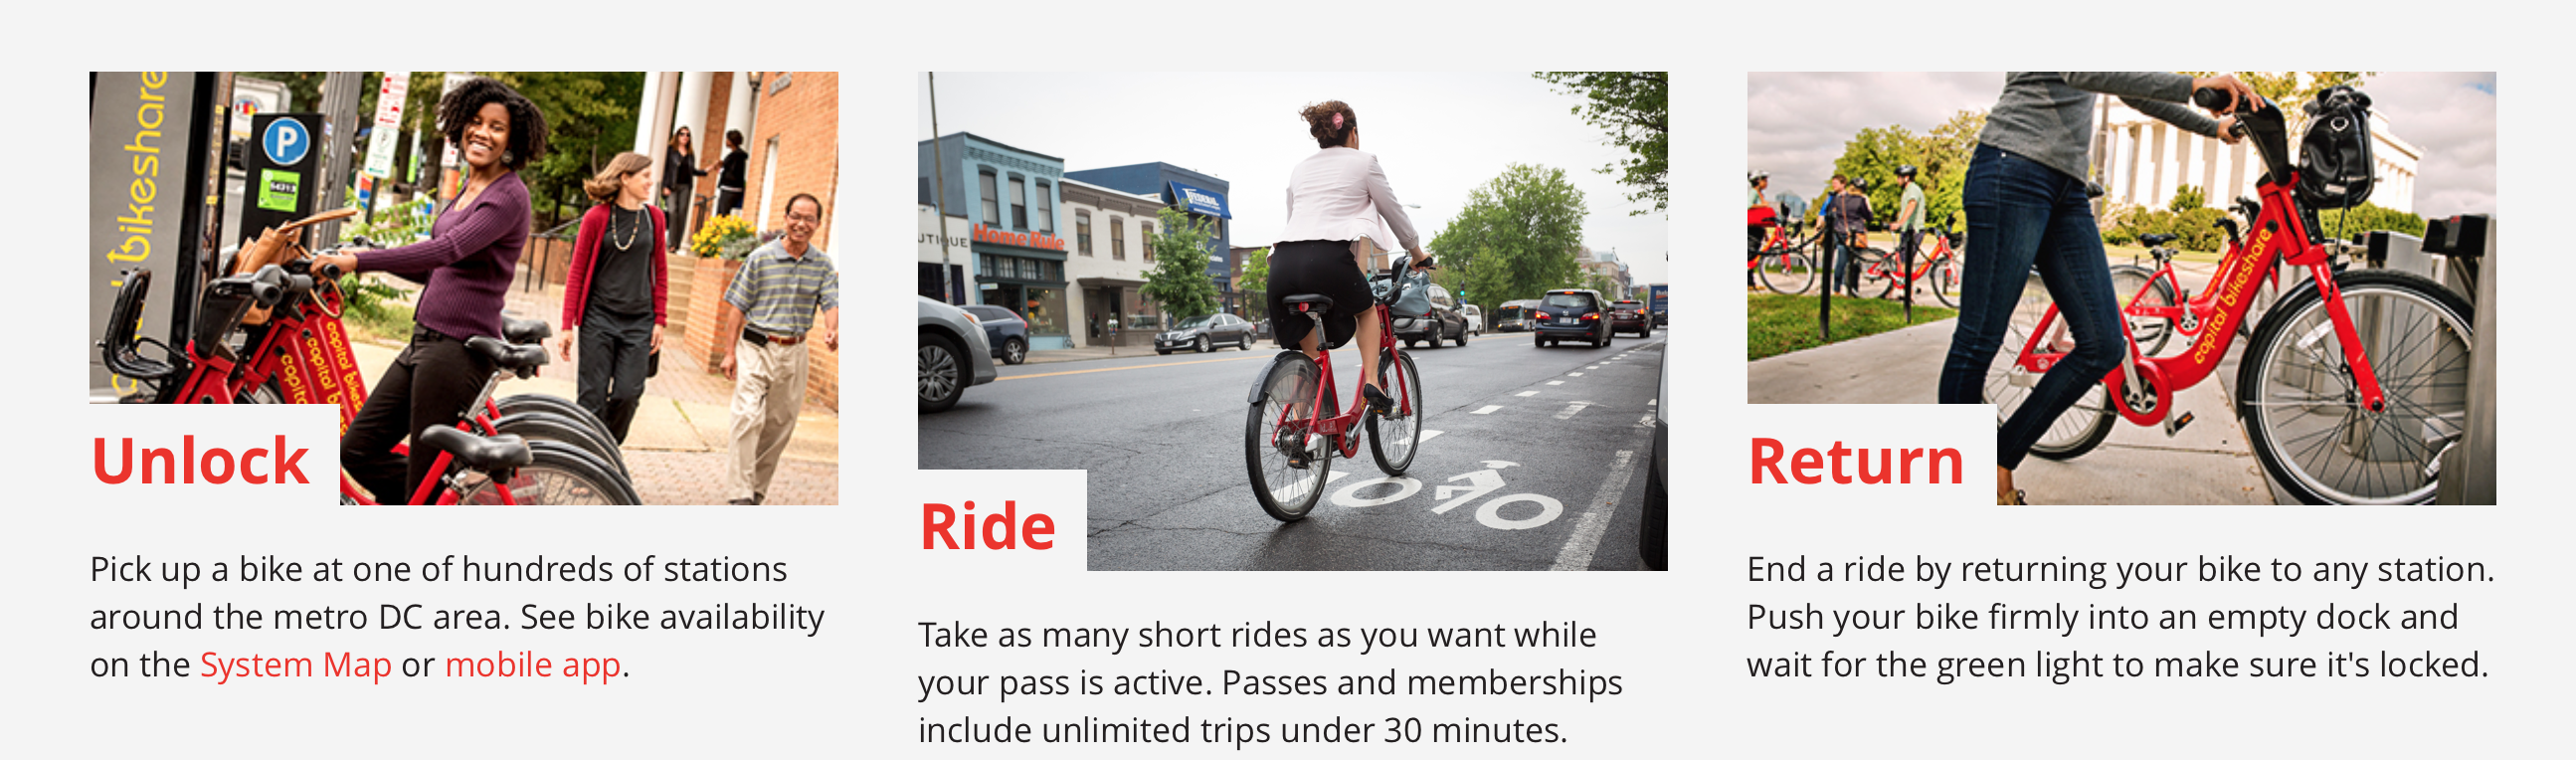
\includegraphics{fig/BSS.png}
\caption{bike\_sharing}
\end{figure}

Main Theme: Multiple Linear Regression, Subset Selection, Polynomial
Regression

\subsubsection{Overview}\label{overview}

You are hired by the administrators of the
\href{https://www.capitalbikeshare.com}{Capital Bikeshare program}
program in Washington D.C., to \textbf{help them predict the hourly
demand for rental bikes} and \textbf{give them suggestions on how to
increase their revenue}. Your task is to prepare a short report
summarizing your findings and make recommendations.

The predicted hourly demand could be used for planning the number of
bikes that need to be available in the system at any given hour of the
day. It costs the program money if bike stations are full and bikes
cannot be returned, or empty and there are no bikes available. You will
use multiple linear regression and polynomial regression and will
explore techniques for subset selection to predict bike usage. The goal
is to build a regression model that can predict the total number of bike
rentals in a given hour of the day, based on all available information
given to you.

An example of a suggestion to increase revenue might be to offer
discounts during certain times of the day either during holidays or
non-holidays. Your suggestions will depend on your observations of the
seasonality of ridership.

The data for this problem were collected from the Capital Bikeshare
program over the course of two years (2011 and 2012).

    \subsubsection{Use only the libraries
below:}\label{use-only-the-libraries-below}

    \begin{Verbatim}[commandchars=\\\{\}]
{\color{incolor}In [{\color{incolor}2}]:} \PY{k+kn}{import} \PY{n+nn}{numpy} \PY{k}{as} \PY{n+nn}{np}
        \PY{k+kn}{import} \PY{n+nn}{pandas} \PY{k}{as} \PY{n+nn}{pd}
        \PY{k+kn}{import} \PY{n+nn}{matplotlib}
        \PY{k+kn}{import} \PY{n+nn}{matplotlib}\PY{n+nn}{.}\PY{n+nn}{pyplot} \PY{k}{as} \PY{n+nn}{plt}
        
        \PY{k+kn}{import} \PY{n+nn}{statsmodels}\PY{n+nn}{.}\PY{n+nn}{api} \PY{k}{as} \PY{n+nn}{sm}
        \PY{k+kn}{from} \PY{n+nn}{statsmodels}\PY{n+nn}{.}\PY{n+nn}{api} \PY{k}{import} \PY{n}{OLS}
        
        \PY{k+kn}{from} \PY{n+nn}{sklearn} \PY{k}{import} \PY{n}{preprocessing}
        \PY{k+kn}{from} \PY{n+nn}{sklearn}\PY{n+nn}{.}\PY{n+nn}{preprocessing} \PY{k}{import} \PY{n}{PolynomialFeatures}
        \PY{k+kn}{from} \PY{n+nn}{sklearn}\PY{n+nn}{.}\PY{n+nn}{metrics} \PY{k}{import} \PY{n}{r2\PYZus{}score}
        \PY{k+kn}{from} \PY{n+nn}{sklearn}\PY{n+nn}{.}\PY{n+nn}{model\PYZus{}selection} \PY{k}{import} \PY{n}{train\PYZus{}test\PYZus{}split}
        
        \PY{k+kn}{from} \PY{n+nn}{pandas}\PY{n+nn}{.}\PY{n+nn}{plotting} \PY{k}{import} \PY{n}{scatter\PYZus{}matrix}
        
        \PY{k+kn}{from} \PY{n+nn}{pandas}\PY{n+nn}{.}\PY{n+nn}{core} \PY{k}{import} \PY{n}{datetools}
        
        \PY{k+kn}{import} \PY{n+nn}{seaborn} \PY{k}{as} \PY{n+nn}{sns}
        
        \PY{k+kn}{import} \PY{n+nn}{itertools}
        \PY{k+kn}{import} \PY{n+nn}{warnings}
        \PY{n}{warnings}\PY{o}{.}\PY{n}{filterwarnings}\PY{p}{(}\PY{l+s+s2}{\PYZdq{}}\PY{l+s+s2}{ignore}\PY{l+s+s2}{\PYZdq{}}\PY{p}{)}
        
        \PY{o}{\PYZpc{}}\PY{k}{matplotlib} inline
\end{Verbatim}


    \begin{Verbatim}[commandchars=\\\{\}]
C:\textbackslash{}Users\textbackslash{}erina\textbackslash{}Anaconda3\textbackslash{}lib\textbackslash{}site-packages\textbackslash{}ipykernel\_launcher.py:16: FutureWarning: The pandas.core.datetools module is deprecated and will be removed in a future version. Please use the pandas.tseries module instead.
  app.launch\_new\_instance()

    \end{Verbatim}

    \subsection{Data Exploration \& Preprocessing, Multiple Linear
Regression, Subset
Selection}\label{data-exploration-preprocessing-multiple-linear-regression-subset-selection}

    \subsubsection{Overview}\label{overview}

The initial data set is provided in the file
\texttt{data/BSS\_hour\_raw.csv}. You will first add features that will
help with the analysis and then separate the data into training and test
sets. Each row in this file represents the number of rides by registered
users and casual users in a given hour of a specific date. There are 12
attributes in total describing besides the number of users the weather
if it is a holiday or not etc:

\begin{itemize}
\tightlist
\item
  \texttt{dteday} (date in the format YYYY-MM-DD, e.g. 2011-01-01)
\item
  \texttt{season} (1 = winter, 2 = spring, 3 = summer, 4 = fall)
\item
  \texttt{hour} (0 for 12 midnight, 1 for 1:00am, 23 for 11:00pm)
\item
  \texttt{weekday} (0 through 6, with 0 denoting Sunday)
\item
  \texttt{holiday} (1 = the day is a holiday, 0 = otherwise)
\item
  \texttt{weather}

  \begin{itemize}
  \tightlist
  \item
    1: Clear, Few clouds, Partly cloudy, Partly cloudy
  \item
    2: Mist + Cloudy, Mist + Broken clouds, Mist + Few clouds, Mist
  \item
    3: Light Snow, Light Rain + Thunderstorm
  \item
    4: Heavy Rain + Thunderstorm + Mist, Snow + Fog
  \end{itemize}
\item
  \texttt{temp} (temperature in Celsius)
\item
  \texttt{atemp} (apparent temperature, or relative outdoor temperature,
  in Celsius)
\item
  \texttt{hum} (relative humidity)
\item
  \texttt{windspeed} (wind speed)
\item
  \texttt{casual} (number of rides that day made by casual riders, not
  registered in the system)
\item
  \texttt{registered} (number of rides that day made by registered
  riders)
\end{itemize}

    \subsubsection{General Hints}\label{general-hints}

\begin{itemize}
\tightlist
\item
  Use pandas .describe() to see statistics for the dataset.
\item
  When performing manipulations on column data it is useful and often
  more efficient to write a function and apply this function to the
  column as a whole without the need for iterating through the elements.
\item
  A scatterplot matrix or correlation matrix are both good ways to see
  dependencies between multiple variables.
\item
  For Question 2, a very useful pandas method is .groupby(). Make sure
  you aggregate the rest of the columns in a meaningful way. Print the
  dataframe to make sure all variables/columns are there!
\end{itemize}

\subsubsection{Resources}\label{resources}

http://pandas.pydata.org/pandas-docs/stable/generated/pandas.to\_datetime.html

     Question 1: Data Read-In and Cleaning

In this section, we read in the data and begin one of the most important
analytic steps: verifying that the data is what it claims to be.

\textbf{1.1} Load the dataset from the csv file
\texttt{data/BSS\_hour\_raw.csv} into a pandas dataframe that you name
\texttt{bikes\_df}. Do any of the variables' ranges or averages seem
suspect? Do the data types make sense?

\textbf{1.2} Notice that the variable in column \texttt{dteday} is a
pandas \texttt{object}, which is \textbf{not} useful when you want to
extract the elements of the date such as the year, month, and day.
Convert \texttt{dteday} into a \texttt{datetime} object to prepare it
for later analysis.

\textbf{1.3} Create three new columns in the dataframe: - \texttt{year}
with 0 for 2011, 1 for 2012, etc. - \texttt{month} with 1 through 12,
with 1 denoting January. - \texttt{counts} with the total number of bike
rentals for that \textbf{hour} (this is the response variable for
later).

    \subsubsection{Answers}\label{answers}

    \paragraph{\texorpdfstring{\textbf{1.1} Load the dataset from the csv
file \texttt{data/BSS\_hour\_raw.csv} into a pandas dataframe that you
name \texttt{bikes\_df}. Do any of the variables' ranges or averages
seem suspect? Do the data types make
sense?}{1.1 Load the dataset from the csv file data/BSS\_hour\_raw.csv into a pandas dataframe that you name bikes\_df. Do any of the variables' ranges or averages seem suspect? Do the data types make sense?}}\label{load-the-dataset-from-the-csv-file-databss_hour_raw.csv-into-a-pandas-dataframe-that-you-name-bikes_df.-do-any-of-the-variables-ranges-or-averages-seem-suspect-do-the-data-types-make-sense}

    \begin{Verbatim}[commandchars=\\\{\}]
{\color{incolor}In [{\color{incolor}3}]:} \PY{n}{bikes\PYZus{}df} \PY{o}{=} \PY{n}{pd}\PY{o}{.}\PY{n}{read\PYZus{}csv}\PY{p}{(}\PY{l+s+s1}{\PYZsq{}}\PY{l+s+s1}{data/BSS\PYZus{}hour\PYZus{}raw.csv}\PY{l+s+s1}{\PYZsq{}}\PY{p}{,} \PY{n}{sep}\PY{o}{=}\PY{l+s+s2}{\PYZdq{}}\PY{l+s+s2}{,}\PY{l+s+s2}{\PYZdq{}}\PY{p}{)}
        \PY{n}{display}\PY{p}{(}\PY{n}{bikes\PYZus{}df}\PY{o}{.}\PY{n}{head}\PY{p}{(}\PY{p}{)}\PY{p}{)}
\end{Verbatim}


    
    \begin{verbatim}
       dteday  season  hour  holiday  weekday  workingday  weather  temp  \
0  2011-01-01       1     0        0        6           0        1  0.24   
1  2011-01-01       1     1        0        6           0        1  0.22   
2  2011-01-01       1     2        0        6           0        1  0.22   
3  2011-01-01       1     3        0        6           0        1  0.24   
4  2011-01-01       1     4        0        6           0        1  0.24   

    atemp   hum  windspeed  casual  registered  
0  0.2879  0.81        0.0       3          13  
1  0.2727  0.80        0.0       8          32  
2  0.2727  0.80        0.0       5          27  
3  0.2879  0.75        0.0       3          10  
4  0.2879  0.75        0.0       0           1  
    \end{verbatim}

    
    \begin{Verbatim}[commandchars=\\\{\}]
{\color{incolor}In [{\color{incolor}4}]:} \PY{n}{bikes\PYZus{}df}\PY{o}{.}\PY{n}{describe}\PY{p}{(}\PY{p}{)}
\end{Verbatim}


\begin{Verbatim}[commandchars=\\\{\}]
{\color{outcolor}Out[{\color{outcolor}4}]:}              season          hour       holiday       weekday    workingday  \textbackslash{}
        count  17379.000000  17379.000000  17379.000000  17379.000000  17379.000000   
        mean       2.501640     11.546752      0.028770      3.003683      0.682721   
        std        1.106918      6.914405      0.167165      2.005771      0.465431   
        min        1.000000      0.000000      0.000000      0.000000      0.000000   
        25\%        2.000000      6.000000      0.000000      1.000000      0.000000   
        50\%        3.000000     12.000000      0.000000      3.000000      1.000000   
        75\%        3.000000     18.000000      0.000000      5.000000      1.000000   
        max        4.000000     23.000000      1.000000      6.000000      1.000000   
        
                    weather          temp         atemp           hum     windspeed  \textbackslash{}
        count  17379.000000  17379.000000  17379.000000  17379.000000  17379.000000   
        mean       1.425283      0.496987      0.475775      0.627229      0.190098   
        std        0.639357      0.192556      0.171850      0.192930      0.122340   
        min        1.000000      0.020000      0.000000      0.000000      0.000000   
        25\%        1.000000      0.340000      0.333300      0.480000      0.104500   
        50\%        1.000000      0.500000      0.484800      0.630000      0.194000   
        75\%        2.000000      0.660000      0.621200      0.780000      0.253700   
        max        4.000000      1.000000      1.000000      1.000000      0.850700   
        
                     casual    registered  
        count  17379.000000  17379.000000  
        mean      35.676218    153.786869  
        std       49.305030    151.357286  
        min        0.000000      0.000000  
        25\%        4.000000     34.000000  
        50\%       17.000000    115.000000  
        75\%       48.000000    220.000000  
        max      367.000000    886.000000  
\end{Verbatim}
            
    \begin{Verbatim}[commandchars=\\\{\}]
{\color{incolor}In [{\color{incolor}5}]:} \PY{c+c1}{\PYZsh{} your code here}
        \PY{n}{bikes\PYZus{}df}\PY{o}{.}\PY{n}{loc}\PY{p}{[}\PY{n}{bikes\PYZus{}df}\PY{p}{[}\PY{l+s+s1}{\PYZsq{}}\PY{l+s+s1}{registered}\PY{l+s+s1}{\PYZsq{}}\PY{p}{]} \PY{o}{==} \PY{l+m+mf}{886.00}\PY{p}{]}
\end{Verbatim}


\begin{Verbatim}[commandchars=\\\{\}]
{\color{outcolor}Out[{\color{outcolor}5}]:}            dteday  season  hour  holiday  weekday  workingday  weather  temp  \textbackslash{}
        14773  2012-09-12       3    18        0        3           1        1  0.66   
        
                atemp   hum  windspeed  casual  registered  
        14773  0.6212  0.44     0.2537      91         886  
\end{Verbatim}
            
    \begin{Verbatim}[commandchars=\\\{\}]
{\color{incolor}In [{\color{incolor}6}]:} \PY{n}{summer\PYZus{}df} \PY{o}{=} \PY{n}{bikes\PYZus{}df}\PY{o}{.}\PY{n}{loc}\PY{p}{[}\PY{n}{bikes\PYZus{}df}\PY{p}{[}\PY{l+s+s1}{\PYZsq{}}\PY{l+s+s1}{weather}\PY{l+s+s1}{\PYZsq{}}\PY{p}{]} \PY{o}{==} \PY{l+m+mi}{1}\PY{p}{]}
        \PY{n}{display}\PY{p}{(}\PY{n}{summer\PYZus{}df}\PY{o}{.}\PY{n}{head}\PY{p}{(}\PY{p}{)}\PY{p}{)}
\end{Verbatim}


    
    \begin{verbatim}
       dteday  season  hour  holiday  weekday  workingday  weather  temp  \
0  2011-01-01       1     0        0        6           0        1  0.24   
1  2011-01-01       1     1        0        6           0        1  0.22   
2  2011-01-01       1     2        0        6           0        1  0.22   
3  2011-01-01       1     3        0        6           0        1  0.24   
4  2011-01-01       1     4        0        6           0        1  0.24   

    atemp   hum  windspeed  casual  registered  
0  0.2879  0.81        0.0       3          13  
1  0.2727  0.80        0.0       8          32  
2  0.2727  0.80        0.0       5          27  
3  0.2879  0.75        0.0       3          10  
4  0.2879  0.75        0.0       0           1  
    \end{verbatim}

    
    \textbf{Answer}\\
The majority of the data makes sense -\/- rides spike on holidays, there
are more riders in the spring/summer/fall months than winter, and the
highest volume of rides occur during the workday. However, the
temperature seems to be skewed. Our summary shows an average temperature
of \(49^o\) C, which is \(120^o\) F. In Washington, DC, average
temperatures in July are \(80^o\)F/\(20^o\)C, and in January the
averages are \(38^o\)F/\(4^o\)C. This tells us the data is skewed or
some sort of scale is off. THe high temperature value is consistent
across individual data points.

    \paragraph{\texorpdfstring{\textbf{1.2} Notice that the variable in
column \texttt{dteday} is a pandas \texttt{object}, which is
\textbf{not} useful when you want to extract the elements of the date
such as the year, month, and day. Convert \texttt{dteday} into a
\texttt{datetime} object to prepare it for later
analysis.}{1.2 Notice that the variable in column dteday is a pandas object, which is not useful when you want to extract the elements of the date such as the year, month, and day. Convert dteday into a datetime object to prepare it for later analysis.}}\label{notice-that-the-variable-in-column-dteday-is-a-pandas-object-which-is-not-useful-when-you-want-to-extract-the-elements-of-the-date-such-as-the-year-month-and-day.-convert-dteday-into-a-datetime-object-to-prepare-it-for-later-analysis.}

    \begin{Verbatim}[commandchars=\\\{\}]
{\color{incolor}In [{\color{incolor}7}]:} \PY{n}{bikes\PYZus{}df}\PY{p}{[}\PY{l+s+s1}{\PYZsq{}}\PY{l+s+s1}{dteday}\PY{l+s+s1}{\PYZsq{}}\PY{p}{]}\PY{o}{=} \PY{n}{pd}\PY{o}{.}\PY{n}{to\PYZus{}datetime}\PY{p}{(}\PY{n}{bikes\PYZus{}df}\PY{p}{[}\PY{l+s+s1}{\PYZsq{}}\PY{l+s+s1}{dteday}\PY{l+s+s1}{\PYZsq{}}\PY{p}{]}\PY{p}{)}
        \PY{n}{display}\PY{p}{(}\PY{n}{bikes\PYZus{}df}\PY{o}{.}\PY{n}{dteday}\PY{o}{.}\PY{n}{head}\PY{p}{(}\PY{p}{)}\PY{p}{)}
\end{Verbatim}


    
    \begin{verbatim}
0   2011-01-01
1   2011-01-01
2   2011-01-01
3   2011-01-01
4   2011-01-01
Name: dteday, dtype: datetime64[ns]
    \end{verbatim}

    
    \paragraph{\texorpdfstring{\textbf{1.3} Create three new columns in the
dataframe:}{1.3 Create three new columns in the dataframe:}}\label{create-three-new-columns-in-the-dataframe}

\begin{itemize}
\tightlist
\item
  \texttt{year} with 0 for 2011, 1 for 2012, etc.
\item
  \texttt{month} with 1 through 12, with 1 denoting January.
\item
  \texttt{counts} with the total number of bike rentals for that hour
  (this is the response variable for later).
\end{itemize}

    \begin{Verbatim}[commandchars=\\\{\}]
{\color{incolor}In [{\color{incolor}8}]:} \PY{n}{bikes\PYZus{}df}\PY{p}{[}\PY{l+s+s1}{\PYZsq{}}\PY{l+s+s1}{year}\PY{l+s+s1}{\PYZsq{}}\PY{p}{]}\PY{o}{=} \PY{n}{pd}\PY{o}{.}\PY{n}{DatetimeIndex}\PY{p}{(}\PY{n}{bikes\PYZus{}df}\PY{p}{[}\PY{l+s+s1}{\PYZsq{}}\PY{l+s+s1}{dteday}\PY{l+s+s1}{\PYZsq{}}\PY{p}{]}\PY{p}{)}\PY{o}{.}\PY{n}{year}
        \PY{n}{bikes\PYZus{}df}\PY{p}{[}\PY{l+s+s1}{\PYZsq{}}\PY{l+s+s1}{month}\PY{l+s+s1}{\PYZsq{}}\PY{p}{]}\PY{o}{=} \PY{n}{pd}\PY{o}{.}\PY{n}{DatetimeIndex}\PY{p}{(}\PY{n}{bikes\PYZus{}df}\PY{p}{[}\PY{l+s+s1}{\PYZsq{}}\PY{l+s+s1}{dteday}\PY{l+s+s1}{\PYZsq{}}\PY{p}{]}\PY{p}{)}\PY{o}{.}\PY{n}{month}
        \PY{n}{bikes\PYZus{}df}\PY{p}{[}\PY{l+s+s1}{\PYZsq{}}\PY{l+s+s1}{year}\PY{l+s+s1}{\PYZsq{}}\PY{p}{]}\PY{o}{=} \PY{n}{bikes\PYZus{}df}\PY{p}{[}\PY{l+s+s1}{\PYZsq{}}\PY{l+s+s1}{year}\PY{l+s+s1}{\PYZsq{}}\PY{p}{]}\PY{o}{.}\PY{n}{map}\PY{p}{(}\PY{p}{\PYZob{}}\PY{l+m+mi}{2012}\PY{p}{:}\PY{l+m+mi}{1}\PY{p}{,}\PY{l+m+mi}{2011}\PY{p}{:}\PY{l+m+mi}{0}\PY{p}{\PYZcb{}}\PY{p}{)}
        \PY{n}{bikes\PYZus{}df}\PY{p}{[}\PY{l+s+s1}{\PYZsq{}}\PY{l+s+s1}{counts}\PY{l+s+s1}{\PYZsq{}}\PY{p}{]}\PY{o}{=}\PY{n}{bikes\PYZus{}df}\PY{o}{.}\PY{n}{casual}\PY{o}{+}\PY{n}{bikes\PYZus{}df}\PY{o}{.}\PY{n}{registered}
        \PY{n}{display}\PY{p}{(}\PY{n}{bikes\PYZus{}df}\PY{o}{.}\PY{n}{head}\PY{p}{(}\PY{p}{)}\PY{p}{)}
\end{Verbatim}


    
    \begin{verbatim}
      dteday  season  hour  holiday  weekday  workingday  weather  temp  \
0 2011-01-01       1     0        0        6           0        1  0.24   
1 2011-01-01       1     1        0        6           0        1  0.22   
2 2011-01-01       1     2        0        6           0        1  0.22   
3 2011-01-01       1     3        0        6           0        1  0.24   
4 2011-01-01       1     4        0        6           0        1  0.24   

    atemp   hum  windspeed  casual  registered  year  month  counts  
0  0.2879  0.81        0.0       3          13     0      1      16  
1  0.2727  0.80        0.0       8          32     0      1      40  
2  0.2727  0.80        0.0       5          27     0      1      32  
3  0.2879  0.75        0.0       3          10     0      1      13  
4  0.2879  0.75        0.0       0           1     0      1       1  
    \end{verbatim}

    
     Question 2: Exploratory Data Analysis.

In this question, we continue validating the data, and begin hunting for
patterns in ridership that shed light on who uses the service and why.

\textbf{2.1} Use pandas' \texttt{scatter\_matrix} command to visualize
the inter-dependencies among all predictors in the dataset. Note and
comment on any strongly related variables. {[}This will take several
minutes to run. You may wish to comment it out until your final
submission, or only plot a randomly-selected 10\% of the rows{]}

\textbf{2.2} Make a plot showing the \emph{average} number of casual and
registered riders during each hour of the day. \texttt{.groupby} and
\texttt{.aggregate} should make this task easy. Comment on the trends
you observe.

\textbf{2.3} Use the variable \texttt{weather} to show how each weather
category affects the relationships in question 2.2. What do you observe?

\textbf{2.4} Make a new dataframe with the following subset of
attributes from the previous dataset and with each entry being just
\textbf{one} day:

\begin{itemize}
\tightlist
\item
  \texttt{dteday}, the timestamp for that day (fine to set to noon or
  any other time)
\item
  \texttt{weekday}, the day of the week
\item
  \texttt{weather}, the most severe weather that day
\item
  \texttt{season}, the season that day falls in
\item
  \texttt{temp}, the average temperature (normalized)
\item
  \texttt{atemp}, the average atemp that day (normalized)
\item
  \texttt{windspeed}, the average windspeed that day (normalized)
\item
  \texttt{hum}, the average humidity that day (normalized)
\item
  \texttt{casual}, the \textbf{total} number of rentals by casual users
\item
  \texttt{registered}, the \textbf{total} number of rentals by
  registered users
\item
  \texttt{counts}, the \textbf{total} number of rentals of that day
\end{itemize}

Name this dataframe \texttt{bikes\_by\_day}.

Make a plot showing the \emph{distribution} of the number of casual and
registered riders on each day of the week.

\textbf{2.5} Use \texttt{bikes\_by\_day} to visualize how the
distribution of \textbf{total number of rides} per day (casual and
registered riders combined) varies with the \textbf{season}. Do you see
any \textbf{outliers}? Here we use the pyplot's boxplot function
definition of an outlier as any value 1.5 times the IQR above the 75th
percentile or 1.5 times the IQR below the 25th percentiles. If you see
any outliers, identify those dates and investigate if they are a chance
occurence, an error in the data collection, or a significant event (an
online search of those date(s) might help).

    \subsubsection{Answers}\label{answers}

    \paragraph{\texorpdfstring{\textbf{2.1} Use pandas'
\texttt{scatter\_matrix} command to visualize the inter-dependencies
among all predictors in the dataset. Note and comment on any strongly
related variables. {[}This will take several minutes to run. You may
wish to comment it out until your final submission, or only plot a
randomly-selected 10\% of the
rows{]}}{2.1 Use pandas' scatter\_matrix command to visualize the inter-dependencies among all predictors in the dataset. Note and comment on any strongly related variables. {[}This will take several minutes to run. You may wish to comment it out until your final submission, or only plot a randomly-selected 10\% of the rows{]}}}\label{use-pandas-scatter_matrix-command-to-visualize-the-inter-dependencies-among-all-predictors-in-the-dataset.-note-and-comment-on-any-strongly-related-variables.-this-will-take-several-minutes-to-run.-you-may-wish-to-comment-it-out-until-your-final-submission-or-only-plot-a-randomly-selected-10-of-the-rows}

    \begin{Verbatim}[commandchars=\\\{\}]
{\color{incolor}In [{\color{incolor}9}]:} \PY{n}{scatter\PYZus{}matrix}\PY{p}{(}\PY{n}{bikes\PYZus{}df}\PY{p}{,} \PY{n}{alpha} \PY{o}{=} \PY{l+m+mf}{0.3}\PY{p}{,} \PY{n}{figsize}\PY{o}{=}\PY{p}{(}\PY{l+m+mi}{20}\PY{p}{,}\PY{l+m+mi}{20}\PY{p}{)}\PY{p}{)}\PY{p}{;}
\end{Verbatim}


    \begin{center}
    \adjustimage{max size={0.9\linewidth}{0.9\paperheight}}{output_25_0.png}
    \end{center}
    { \hspace*{\fill} \\}
    
    \textbf{Answer}\\
We don't see any surprising relationships. Most notably, counts
increases during daytime hours and is higher during late spring, summer,
and early fall months. Additionally, counts is closely realted to the
weather type, with significantly higher values when the weather is rated
as "1" or "2".

    \paragraph{\texorpdfstring{\textbf{2.2} Make a plot showing the
\emph{average} number of casual and registered riders during each hour
of the day. \texttt{.groupby} and \texttt{.aggregate} should make this
task easy. Comment on the trends you
observe.}{2.2 Make a plot showing the average number of casual and registered riders during each hour of the day. .groupby and .aggregate should make this task easy. Comment on the trends you observe.}}\label{make-a-plot-showing-the-average-number-of-casual-and-registered-riders-during-each-hour-of-the-day.-.groupby-and-.aggregate-should-make-this-task-easy.-comment-on-the-trends-you-observe.}

    \begin{Verbatim}[commandchars=\\\{\}]
{\color{incolor}In [{\color{incolor}10}]:} \PY{n}{hour\PYZus{}casual\PYZus{}mean} \PY{o}{=} \PY{n}{bikes\PYZus{}df}\PY{o}{.}\PY{n}{groupby}\PY{p}{(}\PY{l+s+s1}{\PYZsq{}}\PY{l+s+s1}{hour}\PY{l+s+s1}{\PYZsq{}}\PY{p}{)}\PY{o}{.}\PY{n}{agg}\PY{p}{(}\PY{p}{\PYZob{}}\PY{l+s+s1}{\PYZsq{}}\PY{l+s+s1}{casual}\PY{l+s+s1}{\PYZsq{}}\PY{p}{:}\PY{l+s+s1}{\PYZsq{}}\PY{l+s+s1}{mean}\PY{l+s+s1}{\PYZsq{}}\PY{p}{\PYZcb{}}\PY{p}{)}
         \PY{n}{hour\PYZus{}registered\PYZus{}mean}\PY{o}{=} \PY{n}{bikes\PYZus{}df}\PY{o}{.}\PY{n}{groupby}\PY{p}{(}\PY{l+s+s1}{\PYZsq{}}\PY{l+s+s1}{hour}\PY{l+s+s1}{\PYZsq{}}\PY{p}{)}\PY{o}{.}\PY{n}{agg}\PY{p}{(}\PY{p}{\PYZob{}}\PY{l+s+s1}{\PYZsq{}}\PY{l+s+s1}{registered}\PY{l+s+s1}{\PYZsq{}}\PY{p}{:}\PY{l+s+s1}{\PYZsq{}}\PY{l+s+s1}{mean}\PY{l+s+s1}{\PYZsq{}}\PY{p}{\PYZcb{}}\PY{p}{)}
\end{Verbatim}


    \begin{Verbatim}[commandchars=\\\{\}]
{\color{incolor}In [{\color{incolor}11}]:} \PY{n}{avg\PYZus{}hour\PYZus{}frames} \PY{o}{=} \PY{p}{[}\PY{n}{hour\PYZus{}casual\PYZus{}mean}\PY{p}{,}\PY{n}{hour\PYZus{}registered\PYZus{}mean}\PY{p}{]}
         \PY{n}{avg\PYZus{}hour\PYZus{}df} \PY{o}{=} \PY{n}{pd}\PY{o}{.}\PY{n}{concat}\PY{p}{(}\PY{n}{avg\PYZus{}hour\PYZus{}frames}\PY{p}{,} \PY{n}{axis} \PY{o}{=} \PY{l+m+mi}{1}\PY{p}{)}
\end{Verbatim}


    \begin{Verbatim}[commandchars=\\\{\}]
{\color{incolor}In [{\color{incolor}12}]:} \PY{n}{user\PYZus{}plot} \PY{o}{=} \PY{n}{avg\PYZus{}hour\PYZus{}df}\PY{o}{.}\PY{n}{plot}\PY{p}{(}\PY{n}{kind}\PY{o}{=}\PY{l+s+s1}{\PYZsq{}}\PY{l+s+s1}{bar}\PY{l+s+s1}{\PYZsq{}}\PY{p}{,} \PY{n}{title} \PY{o}{=}\PY{l+s+s2}{\PYZdq{}}\PY{l+s+s2}{Average Users Per Hour}\PY{l+s+s2}{\PYZdq{}}\PY{p}{,} \PY{n}{figsize}\PY{o}{=}\PY{p}{(}\PY{l+m+mi}{15}\PY{p}{,} \PY{l+m+mi}{10}\PY{p}{)}\PY{p}{,} \PY{n}{legend}\PY{o}{=}\PY{k+kc}{True}\PY{p}{,} \PY{n}{fontsize}\PY{o}{=}\PY{l+m+mi}{12}\PY{p}{)}
         \PY{n}{user\PYZus{}plot}\PY{o}{.}\PY{n}{set\PYZus{}xlabel}\PY{p}{(}\PY{l+s+s2}{\PYZdq{}}\PY{l+s+s2}{Hour}\PY{l+s+s2}{\PYZdq{}}\PY{p}{,} \PY{n}{fontsize}\PY{o}{=}\PY{l+m+mi}{12}\PY{p}{)}
         \PY{n}{user\PYZus{}plot}\PY{o}{.}\PY{n}{set\PYZus{}ylabel}\PY{p}{(}\PY{l+s+s2}{\PYZdq{}}\PY{l+s+s2}{Average Users}\PY{l+s+s2}{\PYZdq{}}\PY{p}{,} \PY{n}{fontsize}\PY{o}{=}\PY{l+m+mi}{12}\PY{p}{)}
         \PY{n}{plt}\PY{o}{.}\PY{n}{show}\PY{p}{(}\PY{p}{)}
\end{Verbatim}


    \begin{center}
    \adjustimage{max size={0.9\linewidth}{0.9\paperheight}}{output_30_0.png}
    \end{center}
    { \hspace*{\fill} \\}
    
    \textbf{Answer}\\
We can easily observe that rides for registered users spike from
0700-0900 and again from 1600-1900, which generally aligns with rush
hour. This makes sense, since registered users likely rely on the bike
share as a means of commuting. Casual users spike from 1200 to 1800,
indicating that they are likely tourists who are using the bike share to
see DC or get to an attraction.

    \paragraph{\texorpdfstring{\textbf{2.3} Use the variable
\texttt{weather} to show how each weather category affects the
relationships in question 2.2. What do you
observe?}{2.3 Use the variable weather to show how each weather category affects the relationships in question 2.2. What do you observe?}}\label{use-the-variable-weather-to-show-how-each-weather-category-affects-the-relationships-in-question-2.2.-what-do-you-observe}

    \begin{Verbatim}[commandchars=\\\{\}]
{\color{incolor}In [{\color{incolor}13}]:} \PY{c+c1}{\PYZsh{} sort into data frames for each weather type}
         \PY{n}{weather1\PYZus{}df} \PY{o}{=} \PY{n}{bikes\PYZus{}df}\PY{o}{.}\PY{n}{loc}\PY{p}{[}\PY{n}{bikes\PYZus{}df}\PY{p}{[}\PY{l+s+s1}{\PYZsq{}}\PY{l+s+s1}{weather}\PY{l+s+s1}{\PYZsq{}}\PY{p}{]} \PY{o}{==} \PY{l+m+mi}{1}\PY{p}{]}
         \PY{n}{weather2\PYZus{}df} \PY{o}{=} \PY{n}{bikes\PYZus{}df}\PY{o}{.}\PY{n}{loc}\PY{p}{[}\PY{n}{bikes\PYZus{}df}\PY{p}{[}\PY{l+s+s1}{\PYZsq{}}\PY{l+s+s1}{weather}\PY{l+s+s1}{\PYZsq{}}\PY{p}{]} \PY{o}{==} \PY{l+m+mi}{2}\PY{p}{]}
         \PY{n}{weather3\PYZus{}df} \PY{o}{=} \PY{n}{bikes\PYZus{}df}\PY{o}{.}\PY{n}{loc}\PY{p}{[}\PY{n}{bikes\PYZus{}df}\PY{p}{[}\PY{l+s+s1}{\PYZsq{}}\PY{l+s+s1}{weather}\PY{l+s+s1}{\PYZsq{}}\PY{p}{]} \PY{o}{==} \PY{l+m+mi}{3}\PY{p}{]}
         \PY{n}{weather4\PYZus{}df} \PY{o}{=} \PY{n}{bikes\PYZus{}df}\PY{o}{.}\PY{n}{loc}\PY{p}{[}\PY{n}{bikes\PYZus{}df}\PY{p}{[}\PY{l+s+s1}{\PYZsq{}}\PY{l+s+s1}{weather}\PY{l+s+s1}{\PYZsq{}}\PY{p}{]} \PY{o}{==} \PY{l+m+mi}{4}\PY{p}{]}
\end{Verbatim}


    \begin{Verbatim}[commandchars=\\\{\}]
{\color{incolor}In [{\color{incolor}14}]:} \PY{n}{mean\PYZus{}weather1} \PY{o}{=} \PY{n}{weather1\PYZus{}df}\PY{o}{.}\PY{n}{groupby}\PY{p}{(}\PY{p}{[}\PY{l+s+s1}{\PYZsq{}}\PY{l+s+s1}{hour}\PY{l+s+s1}{\PYZsq{}}\PY{p}{]}\PY{p}{)}\PY{o}{.}\PY{n}{agg}\PY{p}{(}\PY{p}{\PYZob{}}\PY{l+s+s1}{\PYZsq{}}\PY{l+s+s1}{casual}\PY{l+s+s1}{\PYZsq{}}\PY{p}{:}\PY{l+s+s1}{\PYZsq{}}\PY{l+s+s1}{mean}\PY{l+s+s1}{\PYZsq{}}\PY{p}{,} \PY{l+s+s1}{\PYZsq{}}\PY{l+s+s1}{registered}\PY{l+s+s1}{\PYZsq{}}\PY{p}{:}\PY{l+s+s1}{\PYZsq{}}\PY{l+s+s1}{mean}\PY{l+s+s1}{\PYZsq{}}\PY{p}{\PYZcb{}}\PY{p}{)}
         \PY{n}{mean\PYZus{}weather2} \PY{o}{=} \PY{n}{weather2\PYZus{}df}\PY{o}{.}\PY{n}{groupby}\PY{p}{(}\PY{p}{[}\PY{l+s+s1}{\PYZsq{}}\PY{l+s+s1}{hour}\PY{l+s+s1}{\PYZsq{}}\PY{p}{]}\PY{p}{)}\PY{o}{.}\PY{n}{agg}\PY{p}{(}\PY{p}{\PYZob{}}\PY{l+s+s1}{\PYZsq{}}\PY{l+s+s1}{casual}\PY{l+s+s1}{\PYZsq{}}\PY{p}{:}\PY{l+s+s1}{\PYZsq{}}\PY{l+s+s1}{mean}\PY{l+s+s1}{\PYZsq{}}\PY{p}{,} \PY{l+s+s1}{\PYZsq{}}\PY{l+s+s1}{registered}\PY{l+s+s1}{\PYZsq{}}\PY{p}{:}\PY{l+s+s1}{\PYZsq{}}\PY{l+s+s1}{mean}\PY{l+s+s1}{\PYZsq{}}\PY{p}{\PYZcb{}}\PY{p}{)}
         \PY{n}{mean\PYZus{}weather3} \PY{o}{=} \PY{n}{weather3\PYZus{}df}\PY{o}{.}\PY{n}{groupby}\PY{p}{(}\PY{p}{[}\PY{l+s+s1}{\PYZsq{}}\PY{l+s+s1}{hour}\PY{l+s+s1}{\PYZsq{}}\PY{p}{]}\PY{p}{)}\PY{o}{.}\PY{n}{agg}\PY{p}{(}\PY{p}{\PYZob{}}\PY{l+s+s1}{\PYZsq{}}\PY{l+s+s1}{casual}\PY{l+s+s1}{\PYZsq{}}\PY{p}{:}\PY{l+s+s1}{\PYZsq{}}\PY{l+s+s1}{mean}\PY{l+s+s1}{\PYZsq{}}\PY{p}{,} \PY{l+s+s1}{\PYZsq{}}\PY{l+s+s1}{registered}\PY{l+s+s1}{\PYZsq{}}\PY{p}{:}\PY{l+s+s1}{\PYZsq{}}\PY{l+s+s1}{mean}\PY{l+s+s1}{\PYZsq{}}\PY{p}{\PYZcb{}}\PY{p}{)}
         \PY{n}{mean\PYZus{}weather4} \PY{o}{=} \PY{n}{weather4\PYZus{}df}\PY{o}{.}\PY{n}{groupby}\PY{p}{(}\PY{p}{[}\PY{l+s+s1}{\PYZsq{}}\PY{l+s+s1}{hour}\PY{l+s+s1}{\PYZsq{}}\PY{p}{]}\PY{p}{)}\PY{o}{.}\PY{n}{agg}\PY{p}{(}\PY{p}{\PYZob{}}\PY{l+s+s1}{\PYZsq{}}\PY{l+s+s1}{casual}\PY{l+s+s1}{\PYZsq{}}\PY{p}{:}\PY{l+s+s1}{\PYZsq{}}\PY{l+s+s1}{mean}\PY{l+s+s1}{\PYZsq{}}\PY{p}{,} \PY{l+s+s1}{\PYZsq{}}\PY{l+s+s1}{registered}\PY{l+s+s1}{\PYZsq{}}\PY{p}{:}\PY{l+s+s1}{\PYZsq{}}\PY{l+s+s1}{mean}\PY{l+s+s1}{\PYZsq{}}\PY{p}{\PYZcb{}}\PY{p}{)}
\end{Verbatim}


    \begin{Verbatim}[commandchars=\\\{\}]
{\color{incolor}In [{\color{incolor}15}]:} \PY{n}{user\PYZus{}plot1} \PY{o}{=} \PY{n}{mean\PYZus{}weather1}\PY{o}{.}\PY{n}{plot}\PY{o}{.}\PY{n}{bar}\PY{p}{(}\PY{n}{rot} \PY{o}{=} \PY{l+m+mi}{0}\PY{p}{,} \PY{n}{title} \PY{o}{=}\PY{l+s+s2}{\PYZdq{}}\PY{l+s+s2}{Average Users Per Hour in Clear to Partly Cloudy Weather}\PY{l+s+s2}{\PYZdq{}}\PY{p}{,} \PY{n}{figsize}\PY{o}{=}\PY{p}{(}\PY{l+m+mi}{10}\PY{p}{,} \PY{l+m+mi}{5}\PY{p}{)}\PY{p}{,} \PY{n}{legend}\PY{o}{=}\PY{k+kc}{True}\PY{p}{,} \PY{n}{fontsize}\PY{o}{=}\PY{l+m+mi}{12}\PY{p}{)}
         \PY{n}{user\PYZus{}plot1}\PY{o}{.}\PY{n}{set\PYZus{}xlabel}\PY{p}{(}\PY{l+s+s2}{\PYZdq{}}\PY{l+s+s2}{Hour}\PY{l+s+s2}{\PYZdq{}}\PY{p}{,} \PY{n}{fontsize}\PY{o}{=}\PY{l+m+mi}{12}\PY{p}{)}
         \PY{n}{user\PYZus{}plot1}\PY{o}{.}\PY{n}{set\PYZus{}ylabel}\PY{p}{(}\PY{l+s+s2}{\PYZdq{}}\PY{l+s+s2}{Average Users}\PY{l+s+s2}{\PYZdq{}}\PY{p}{,} \PY{n}{fontsize}\PY{o}{=}\PY{l+m+mi}{12}\PY{p}{)}
         \PY{n}{user\PYZus{}plot1}\PY{o}{.}\PY{n}{set\PYZus{}yticks}\PY{p}{(}\PY{p}{[}\PY{l+m+mi}{50}\PY{p}{,}\PY{l+m+mi}{100}\PY{p}{,}\PY{l+m+mi}{150}\PY{p}{,}\PY{l+m+mi}{200}\PY{p}{,}\PY{l+m+mi}{250}\PY{p}{,}\PY{l+m+mi}{300}\PY{p}{,}\PY{l+m+mi}{350}\PY{p}{,}\PY{l+m+mi}{400}\PY{p}{,}\PY{l+m+mi}{450}\PY{p}{]}\PY{p}{)}
         \PY{n}{plt}\PY{o}{.}\PY{n}{show}\PY{p}{(}\PY{p}{)}
         
         \PY{n}{user\PYZus{}plot2} \PY{o}{=} \PY{n}{mean\PYZus{}weather2}\PY{o}{.}\PY{n}{plot}\PY{o}{.}\PY{n}{bar}\PY{p}{(}\PY{n}{rot} \PY{o}{=} \PY{l+m+mi}{0}\PY{p}{,} \PY{n}{title} \PY{o}{=}\PY{l+s+s2}{\PYZdq{}}\PY{l+s+s2}{Average Users Per Hour in Cloudy and Misty Weather}\PY{l+s+s2}{\PYZdq{}}\PY{p}{,} \PY{n}{figsize}\PY{o}{=}\PY{p}{(}\PY{l+m+mi}{10}\PY{p}{,} \PY{l+m+mi}{5}\PY{p}{)}\PY{p}{,} \PY{n}{legend}\PY{o}{=}\PY{k+kc}{True}\PY{p}{,} \PY{n}{fontsize}\PY{o}{=}\PY{l+m+mi}{12}\PY{p}{)}
         \PY{n}{user\PYZus{}plot2}\PY{o}{.}\PY{n}{set\PYZus{}xlabel}\PY{p}{(}\PY{l+s+s2}{\PYZdq{}}\PY{l+s+s2}{Hour}\PY{l+s+s2}{\PYZdq{}}\PY{p}{,} \PY{n}{fontsize}\PY{o}{=}\PY{l+m+mi}{12}\PY{p}{)}
         \PY{n}{user\PYZus{}plot2}\PY{o}{.}\PY{n}{set\PYZus{}ylabel}\PY{p}{(}\PY{l+s+s2}{\PYZdq{}}\PY{l+s+s2}{Average Users}\PY{l+s+s2}{\PYZdq{}}\PY{p}{,} \PY{n}{fontsize}\PY{o}{=}\PY{l+m+mi}{12}\PY{p}{)}
         \PY{n}{user\PYZus{}plot2}\PY{o}{.}\PY{n}{set\PYZus{}yticks}\PY{p}{(}\PY{p}{[}\PY{l+m+mi}{50}\PY{p}{,}\PY{l+m+mi}{100}\PY{p}{,}\PY{l+m+mi}{150}\PY{p}{,}\PY{l+m+mi}{200}\PY{p}{,}\PY{l+m+mi}{250}\PY{p}{,}\PY{l+m+mi}{300}\PY{p}{,}\PY{l+m+mi}{350}\PY{p}{,}\PY{l+m+mi}{400}\PY{p}{,}\PY{l+m+mi}{450}\PY{p}{]}\PY{p}{)}
         \PY{n}{plt}\PY{o}{.}\PY{n}{show}\PY{p}{(}\PY{p}{)}
         
         \PY{n}{user\PYZus{}plot3} \PY{o}{=} \PY{n}{mean\PYZus{}weather3}\PY{o}{.}\PY{n}{plot}\PY{o}{.}\PY{n}{bar}\PY{p}{(}\PY{n}{rot} \PY{o}{=} \PY{l+m+mi}{0}\PY{p}{,} \PY{n}{title} \PY{o}{=}\PY{l+s+s2}{\PYZdq{}}\PY{l+s+s2}{Average Users Per Hour in Light Snow or Rain}\PY{l+s+s2}{\PYZdq{}}\PY{p}{,} \PY{n}{figsize}\PY{o}{=}\PY{p}{(}\PY{l+m+mi}{10}\PY{p}{,} \PY{l+m+mi}{5}\PY{p}{)}\PY{p}{,} \PY{n}{legend}\PY{o}{=}\PY{k+kc}{True}\PY{p}{,} \PY{n}{fontsize}\PY{o}{=}\PY{l+m+mi}{12}\PY{p}{)}
         \PY{n}{user\PYZus{}plot3}\PY{o}{.}\PY{n}{set\PYZus{}xlabel}\PY{p}{(}\PY{l+s+s2}{\PYZdq{}}\PY{l+s+s2}{Hour}\PY{l+s+s2}{\PYZdq{}}\PY{p}{,} \PY{n}{fontsize}\PY{o}{=}\PY{l+m+mi}{12}\PY{p}{)}
         \PY{n}{user\PYZus{}plot3}\PY{o}{.}\PY{n}{set\PYZus{}ylabel}\PY{p}{(}\PY{l+s+s2}{\PYZdq{}}\PY{l+s+s2}{Average Users}\PY{l+s+s2}{\PYZdq{}}\PY{p}{,} \PY{n}{fontsize}\PY{o}{=}\PY{l+m+mi}{12}\PY{p}{)}
         \PY{n}{user\PYZus{}plot3}\PY{o}{.}\PY{n}{set\PYZus{}yticks}\PY{p}{(}\PY{p}{[}\PY{l+m+mi}{50}\PY{p}{,}\PY{l+m+mi}{100}\PY{p}{,}\PY{l+m+mi}{150}\PY{p}{,}\PY{l+m+mi}{200}\PY{p}{,}\PY{l+m+mi}{250}\PY{p}{,}\PY{l+m+mi}{300}\PY{p}{,}\PY{l+m+mi}{350}\PY{p}{,}\PY{l+m+mi}{400}\PY{p}{,}\PY{l+m+mi}{450}\PY{p}{]}\PY{p}{)}
         \PY{n}{plt}\PY{o}{.}\PY{n}{show}\PY{p}{(}\PY{p}{)}
         
         \PY{n}{user\PYZus{}plot4} \PY{o}{=} \PY{n}{mean\PYZus{}weather4}\PY{o}{.}\PY{n}{plot}\PY{o}{.}\PY{n}{bar}\PY{p}{(}\PY{n}{rot} \PY{o}{=} \PY{l+m+mi}{0}\PY{p}{,} \PY{n}{title} \PY{o}{=}\PY{l+s+s2}{\PYZdq{}}\PY{l+s+s2}{Average Users Per Hour in Heavy Rain, Thunderstorms, and Fog}\PY{l+s+s2}{\PYZdq{}}\PY{p}{,} \PY{n}{figsize}\PY{o}{=}\PY{p}{(}\PY{l+m+mi}{10}\PY{p}{,} \PY{l+m+mi}{5}\PY{p}{)}\PY{p}{,} \PY{n}{legend}\PY{o}{=}\PY{k+kc}{True}\PY{p}{,} \PY{n}{fontsize}\PY{o}{=}\PY{l+m+mi}{12}\PY{p}{)}
         \PY{n}{user\PYZus{}plot4}\PY{o}{.}\PY{n}{set\PYZus{}xlabel}\PY{p}{(}\PY{l+s+s2}{\PYZdq{}}\PY{l+s+s2}{Hour}\PY{l+s+s2}{\PYZdq{}}\PY{p}{,} \PY{n}{fontsize}\PY{o}{=}\PY{l+m+mi}{12}\PY{p}{)}
         \PY{n}{user\PYZus{}plot4}\PY{o}{.}\PY{n}{set\PYZus{}ylabel}\PY{p}{(}\PY{l+s+s2}{\PYZdq{}}\PY{l+s+s2}{Average Users}\PY{l+s+s2}{\PYZdq{}}\PY{p}{,} \PY{n}{fontsize}\PY{o}{=}\PY{l+m+mi}{12}\PY{p}{)}
         \PY{n}{user\PYZus{}plot4}\PY{o}{.}\PY{n}{set\PYZus{}yticks}\PY{p}{(}\PY{p}{[}\PY{l+m+mi}{50}\PY{p}{,}\PY{l+m+mi}{100}\PY{p}{,}\PY{l+m+mi}{150}\PY{p}{,}\PY{l+m+mi}{200}\PY{p}{,}\PY{l+m+mi}{250}\PY{p}{,}\PY{l+m+mi}{300}\PY{p}{,}\PY{l+m+mi}{350}\PY{p}{,}\PY{l+m+mi}{400}\PY{p}{,}\PY{l+m+mi}{450}\PY{p}{]}\PY{p}{)}
         \PY{n}{user\PYZus{}plot4}\PY{o}{.}\PY{n}{set\PYZus{}xticks}\PY{p}{(}\PY{p}{[}\PY{l+m+mi}{0}\PY{p}{,}\PY{l+m+mi}{1}\PY{p}{,}\PY{l+m+mi}{2}\PY{p}{,}\PY{l+m+mi}{3}\PY{p}{,}\PY{l+m+mi}{4}\PY{p}{,}\PY{l+m+mi}{5}\PY{p}{,}\PY{l+m+mi}{6}\PY{p}{,}\PY{l+m+mi}{7}\PY{p}{,}\PY{l+m+mi}{8}\PY{p}{,}\PY{l+m+mi}{9}\PY{p}{,}\PY{l+m+mi}{10}\PY{p}{,}\PY{l+m+mi}{11}\PY{p}{,}\PY{l+m+mi}{12}\PY{p}{,}\PY{l+m+mi}{13}\PY{p}{,}\PY{l+m+mi}{14}\PY{p}{,}\PY{l+m+mi}{15}\PY{p}{,}\PY{l+m+mi}{16}\PY{p}{,}\PY{l+m+mi}{17}\PY{p}{,}\PY{l+m+mi}{18}\PY{p}{,}\PY{l+m+mi}{19}\PY{p}{,}\PY{l+m+mi}{20}\PY{p}{,}\PY{l+m+mi}{21}\PY{p}{,}\PY{l+m+mi}{22}\PY{p}{,}\PY{l+m+mi}{23}\PY{p}{]}\PY{p}{)}
         \PY{n}{plt}\PY{o}{.}\PY{n}{show}\PY{p}{(}\PY{p}{)}
\end{Verbatim}


    \begin{center}
    \adjustimage{max size={0.9\linewidth}{0.9\paperheight}}{output_35_0.png}
    \end{center}
    { \hspace*{\fill} \\}
    
    \begin{center}
    \adjustimage{max size={0.9\linewidth}{0.9\paperheight}}{output_35_1.png}
    \end{center}
    { \hspace*{\fill} \\}
    
    \begin{center}
    \adjustimage{max size={0.9\linewidth}{0.9\paperheight}}{output_35_2.png}
    \end{center}
    { \hspace*{\fill} \\}
    
    \begin{center}
    \adjustimage{max size={0.9\linewidth}{0.9\paperheight}}{output_35_3.png}
    \end{center}
    { \hspace*{\fill} \\}
    
    \textbf{Answer} We can see that while the trend line generally holds,
the averages begin to fall as weather gets bad (decreasing from 1 to 2,
and from 2 to 3), and riders almost completely drop off during the worst
weather conditions.

    \paragraph{\texorpdfstring{\textbf{2.4} Make a new dataframe with the
following subset of attributes from the previous dataset and with each
entry being just \textbf{one}
day:}{2.4 Make a new dataframe with the following subset of attributes from the previous dataset and with each entry being just one day:}}\label{make-a-new-dataframe-with-the-following-subset-of-attributes-from-the-previous-dataset-and-with-each-entry-being-just-one-day}

\begin{itemize}
\tightlist
\item
  \texttt{dteday}, the timestamp for that day (fine to set to noon or
  any other time)
\item
  \texttt{weekday}, the day of the week
\item
  \texttt{weather}, the most severe weather that day
\item
  \texttt{season}, the season that day falls in
\item
  \texttt{temp}, the average temperature (normalized)
\item
  \texttt{atemp}, the average atemp that day (normalized)
\item
  \texttt{windspeed}, the average windspeed that day (normalized)
\item
  \texttt{hum}, the average humidity that day (normalized)
\item
  \texttt{casual}, the \textbf{total} number of rentals by casual users
\item
  \texttt{registered}, the \textbf{total} number of rentals by
  registered users
\item
  \texttt{counts}, the \textbf{total} number of rentals of that day
\end{itemize}

\paragraph{\texorpdfstring{Name this dataframe
\texttt{bikes\_by\_day}.}{Name this dataframe bikes\_by\_day.}}\label{name-this-dataframe-bikes_by_day.}

\paragraph{\texorpdfstring{Make a plot showing the \emph{distribution}
of the number of casual and registered riders on each day of the
week.}{Make a plot showing the distribution of the number of casual and registered riders on each day of the week.}}\label{make-a-plot-showing-the-distribution-of-the-number-of-casual-and-registered-riders-on-each-day-of-the-week.}

    \begin{Verbatim}[commandchars=\\\{\}]
{\color{incolor}In [{\color{incolor}16}]:} \PY{n}{bikes\PYZus{}by\PYZus{}day} \PY{o}{=} \PY{n}{pd}\PY{o}{.}\PY{n}{DataFrame}\PY{p}{(}\PY{n}{bikes\PYZus{}df}\PY{o}{.}\PY{n}{groupby}\PY{p}{(}\PY{l+s+s1}{\PYZsq{}}\PY{l+s+s1}{dteday}\PY{l+s+s1}{\PYZsq{}}\PY{p}{)}\PY{o}{.}\PY{n}{agg}\PY{p}{(}\PY{p}{\PYZob{}}
             \PY{l+s+s1}{\PYZsq{}}\PY{l+s+s1}{dteday}\PY{l+s+s1}{\PYZsq{}}\PY{p}{:} \PY{n}{np}\PY{o}{.}\PY{n}{min}\PY{p}{,}
             \PY{l+s+s1}{\PYZsq{}}\PY{l+s+s1}{temp}\PY{l+s+s1}{\PYZsq{}}\PY{p}{:} \PY{n}{np}\PY{o}{.}\PY{n}{mean}\PY{p}{,}
             \PY{l+s+s1}{\PYZsq{}}\PY{l+s+s1}{atemp}\PY{l+s+s1}{\PYZsq{}}\PY{p}{:} \PY{n}{np}\PY{o}{.}\PY{n}{mean}\PY{p}{,}
             \PY{l+s+s1}{\PYZsq{}}\PY{l+s+s1}{windspeed}\PY{l+s+s1}{\PYZsq{}}\PY{p}{:} \PY{n}{np}\PY{o}{.}\PY{n}{mean}\PY{p}{,}
             \PY{l+s+s1}{\PYZsq{}}\PY{l+s+s1}{hum}\PY{l+s+s1}{\PYZsq{}}\PY{p}{:} \PY{n}{np}\PY{o}{.}\PY{n}{mean}\PY{p}{,}
             \PY{l+s+s1}{\PYZsq{}}\PY{l+s+s1}{casual}\PY{l+s+s1}{\PYZsq{}}\PY{p}{:} \PY{n}{np}\PY{o}{.}\PY{n}{sum}\PY{p}{,}
             \PY{l+s+s1}{\PYZsq{}}\PY{l+s+s1}{registered}\PY{l+s+s1}{\PYZsq{}}\PY{p}{:} \PY{n}{np}\PY{o}{.}\PY{n}{sum}\PY{p}{,}
             \PY{l+s+s1}{\PYZsq{}}\PY{l+s+s1}{counts}\PY{l+s+s1}{\PYZsq{}}\PY{p}{:} \PY{n}{np}\PY{o}{.}\PY{n}{sum}
         \PY{p}{\PYZcb{}}\PY{p}{)}\PY{p}{)}
         \PY{n}{bikes\PYZus{}by\PYZus{}day2} \PY{o}{=} \PY{n}{pd}\PY{o}{.}\PY{n}{DataFrame}\PY{p}{(}\PY{p}{)}
         \PY{n}{bikes\PYZus{}by\PYZus{}day2}\PY{p}{[}\PY{l+s+s1}{\PYZsq{}}\PY{l+s+s1}{dteday}\PY{l+s+s1}{\PYZsq{}}\PY{p}{]} \PY{o}{=} \PY{n}{pd}\PY{o}{.}\PY{n}{to\PYZus{}datetime}\PY{p}{(}\PY{n}{bikes\PYZus{}df}\PY{p}{[}\PY{l+s+s1}{\PYZsq{}}\PY{l+s+s1}{dteday}\PY{l+s+s1}{\PYZsq{}}\PY{p}{]}\PY{p}{)}
         \PY{n}{bikes\PYZus{}by\PYZus{}day2}\PY{p}{[}\PY{l+s+s1}{\PYZsq{}}\PY{l+s+s1}{weekday}\PY{l+s+s1}{\PYZsq{}}\PY{p}{]} \PY{o}{=} \PY{n}{pd}\PY{o}{.}\PY{n}{DatetimeIndex}\PY{p}{(}\PY{n}{bikes\PYZus{}df}\PY{p}{[}\PY{l+s+s1}{\PYZsq{}}\PY{l+s+s1}{dteday}\PY{l+s+s1}{\PYZsq{}}\PY{p}{]}\PY{p}{)}\PY{o}{.}\PY{n}{weekday} \PY{c+c1}{\PYZsh{}0 = monday, 6 = Sunday}
         \PY{n}{bikes\PYZus{}by\PYZus{}day2}\PY{p}{[}\PY{l+s+s1}{\PYZsq{}}\PY{l+s+s1}{season}\PY{l+s+s1}{\PYZsq{}}\PY{p}{]} \PY{o}{=} \PY{n}{pd}\PY{o}{.}\PY{n}{DatetimeIndex}\PY{p}{(}\PY{n}{bikes\PYZus{}df}\PY{p}{[}\PY{l+s+s1}{\PYZsq{}}\PY{l+s+s1}{dteday}\PY{l+s+s1}{\PYZsq{}}\PY{p}{]}\PY{p}{)}\PY{o}{.}\PY{n}{month}
         \PY{n}{bikes\PYZus{}by\PYZus{}day2}\PY{p}{[}\PY{l+s+s1}{\PYZsq{}}\PY{l+s+s1}{season}\PY{l+s+s1}{\PYZsq{}}\PY{p}{]} \PY{o}{=} \PY{p}{(}\PY{p}{(}\PY{n}{bikes\PYZus{}by\PYZus{}day2}\PY{o}{.}\PY{n}{season}\PY{o}{\PYZpc{}}\PY{k}{12} + 3)//3)\PYZhy{}1 \PYZsh{} 0 = winter, 1 = spring, 2 = summer, 3 = fall
         \PY{n}{bikes\PYZus{}by\PYZus{}day2} \PY{o}{=} \PY{n}{bikes\PYZus{}by\PYZus{}day2}\PY{o}{.}\PY{n}{drop\PYZus{}duplicates}\PY{p}{(}\PY{p}{[}\PY{l+s+s2}{\PYZdq{}}\PY{l+s+s2}{dteday}\PY{l+s+s2}{\PYZdq{}}\PY{p}{]}\PY{p}{)}
         \PY{n}{bikes\PYZus{}by\PYZus{}day2}\PY{o}{.}\PY{n}{set\PYZus{}index}\PY{p}{(}\PY{l+s+s1}{\PYZsq{}}\PY{l+s+s1}{dteday}\PY{l+s+s1}{\PYZsq{}}\PY{p}{)}
         \PY{n}{bikes\PYZus{}by\PYZus{}day} \PY{o}{=} \PY{n}{pd}\PY{o}{.}\PY{n}{merge}\PY{p}{(}\PY{n}{bikes\PYZus{}by\PYZus{}day}\PY{p}{,} \PY{n}{bikes\PYZus{}by\PYZus{}day2}\PY{p}{,} \PY{n}{on}\PY{o}{=}\PY{p}{[}\PY{l+s+s1}{\PYZsq{}}\PY{l+s+s1}{dteday}\PY{l+s+s1}{\PYZsq{}}\PY{p}{]}\PY{p}{)}
         \PY{n}{display}\PY{p}{(}\PY{n}{bikes\PYZus{}by\PYZus{}day}\PY{o}{.}\PY{n}{head}\PY{p}{(}\PY{p}{)}\PY{p}{)}
\end{Verbatim}


    
    \begin{verbatim}
      dteday      temp     atemp  windspeed       hum  casual  registered  \
0 2011-01-01  0.344167  0.363625   0.160446  0.805833     331         654   
1 2011-01-02  0.363478  0.353739   0.248539  0.696087     131         670   
2 2011-01-03  0.196364  0.189405   0.248309  0.437273     120        1229   
3 2011-01-04  0.200000  0.212122   0.160296  0.590435     108        1454   
4 2011-01-05  0.226957  0.229270   0.186900  0.436957      82        1518   

   counts  weekday  season  
0     985        5       0  
1     801        6       0  
2    1349        0       0  
3    1562        1       0  
4    1600        2       0  
    \end{verbatim}

    
    \begin{Verbatim}[commandchars=\\\{\}]
{\color{incolor}In [{\color{incolor}17}]:} \PY{n}{casual\PYZus{}mean} \PY{o}{=} \PY{n}{bikes\PYZus{}by\PYZus{}day}\PY{o}{.}\PY{n}{groupby}\PY{p}{(}\PY{l+s+s1}{\PYZsq{}}\PY{l+s+s1}{weekday}\PY{l+s+s1}{\PYZsq{}}\PY{p}{)}\PY{o}{.}\PY{n}{agg}\PY{p}{(}\PY{p}{\PYZob{}}\PY{l+s+s1}{\PYZsq{}}\PY{l+s+s1}{casual}\PY{l+s+s1}{\PYZsq{}}\PY{p}{:}\PY{l+s+s1}{\PYZsq{}}\PY{l+s+s1}{mean}\PY{l+s+s1}{\PYZsq{}}\PY{p}{\PYZcb{}}\PY{p}{)}
         \PY{n}{registered\PYZus{}mean}\PY{o}{=} \PY{n}{bikes\PYZus{}by\PYZus{}day}\PY{o}{.}\PY{n}{groupby}\PY{p}{(}\PY{l+s+s1}{\PYZsq{}}\PY{l+s+s1}{weekday}\PY{l+s+s1}{\PYZsq{}}\PY{p}{)}\PY{o}{.}\PY{n}{agg}\PY{p}{(}\PY{p}{\PYZob{}}\PY{l+s+s1}{\PYZsq{}}\PY{l+s+s1}{registered}\PY{l+s+s1}{\PYZsq{}}\PY{p}{:}\PY{l+s+s1}{\PYZsq{}}\PY{l+s+s1}{mean}\PY{l+s+s1}{\PYZsq{}}\PY{p}{\PYZcb{}}\PY{p}{)}
\end{Verbatim}


    \begin{Verbatim}[commandchars=\\\{\}]
{\color{incolor}In [{\color{incolor}18}]:} \PY{n}{avg\PYZus{}week\PYZus{}frames} \PY{o}{=} \PY{p}{[}\PY{n}{casual\PYZus{}mean}\PY{p}{,}\PY{n}{registered\PYZus{}mean}\PY{p}{]}
         \PY{n}{avg\PYZus{}week\PYZus{}df} \PY{o}{=} \PY{n}{pd}\PY{o}{.}\PY{n}{concat}\PY{p}{(}\PY{n}{avg\PYZus{}week\PYZus{}frames}\PY{p}{,} \PY{n}{axis} \PY{o}{=} \PY{l+m+mi}{1}\PY{p}{)}
\end{Verbatim}


    \begin{Verbatim}[commandchars=\\\{\}]
{\color{incolor}In [{\color{incolor}19}]:} \PY{n}{user\PYZus{}plot} \PY{o}{=} \PY{n}{avg\PYZus{}week\PYZus{}df}\PY{o}{.}\PY{n}{plot}\PY{p}{(}\PY{n}{kind}\PY{o}{=}\PY{l+s+s1}{\PYZsq{}}\PY{l+s+s1}{bar}\PY{l+s+s1}{\PYZsq{}}\PY{p}{,} \PY{n}{title} \PY{o}{=}\PY{l+s+s2}{\PYZdq{}}\PY{l+s+s2}{Average Users Per Weekday}\PY{l+s+s2}{\PYZdq{}}\PY{p}{,} \PY{n}{figsize}\PY{o}{=}\PY{p}{(}\PY{l+m+mi}{10}\PY{p}{,} \PY{l+m+mi}{8}\PY{p}{)}\PY{p}{,} \PY{n}{legend}\PY{o}{=}\PY{k+kc}{True}\PY{p}{,} \PY{n}{fontsize}\PY{o}{=}\PY{l+m+mi}{12}\PY{p}{)}
         \PY{n}{user\PYZus{}plot}\PY{o}{.}\PY{n}{set\PYZus{}xlabel}\PY{p}{(}\PY{l+s+s2}{\PYZdq{}}\PY{l+s+s2}{Weekday}\PY{l+s+s2}{\PYZdq{}}\PY{p}{,} \PY{n}{fontsize}\PY{o}{=}\PY{l+m+mi}{12}\PY{p}{)}
         \PY{n}{user\PYZus{}plot}\PY{o}{.}\PY{n}{set\PYZus{}ylabel}\PY{p}{(}\PY{l+s+s2}{\PYZdq{}}\PY{l+s+s2}{Average Users}\PY{l+s+s2}{\PYZdq{}}\PY{p}{,} \PY{n}{fontsize}\PY{o}{=}\PY{l+m+mi}{12}\PY{p}{)}
         \PY{n}{plt}\PY{o}{.}\PY{n}{show}\PY{p}{(}\PY{p}{)}
\end{Verbatim}


    \begin{center}
    \adjustimage{max size={0.9\linewidth}{0.9\paperheight}}{output_41_0.png}
    \end{center}
    { \hspace*{\fill} \\}
    
    \textbf{Answer}\\
Registered users are highest during weekdays. Registered users likely
use the bikes to commute to work and run errands, so this makes sense.
Casual users increase on weekends. Generally speaking, more tourists
visit DC on the weekends, so this also makes sense.

    \textbf{2.5} Use \texttt{bikes\_by\_day} to visualize how the
distribution of \textbf{total number of rides} per day (casual and
registered riders combined) varies with the \textbf{season}. Do you see
any \textbf{outliers}? Here we use the pyplot's boxplot function
definition of an outlier as any value 1.5 times the IQR above the 75th
percentile or 1.5 times the IQR below the 25th percentiles. If you see
any outliers, identify those dates and investigate if they are a chance
occurence, an error in the data collection, or a significant event (an
online search of those date(s) might help).

    \begin{Verbatim}[commandchars=\\\{\}]
{\color{incolor}In [{\color{incolor}20}]:} \PY{c+c1}{\PYZsh{} your code here }
         \PY{n}{display}\PY{p}{(}\PY{n}{bikes\PYZus{}by\PYZus{}day}\PY{o}{.}\PY{n}{head}\PY{p}{(}\PY{p}{)}\PY{p}{)}
\end{Verbatim}


    
    \begin{verbatim}
      dteday      temp     atemp  windspeed       hum  casual  registered  \
0 2011-01-01  0.344167  0.363625   0.160446  0.805833     331         654   
1 2011-01-02  0.363478  0.353739   0.248539  0.696087     131         670   
2 2011-01-03  0.196364  0.189405   0.248309  0.437273     120        1229   
3 2011-01-04  0.200000  0.212122   0.160296  0.590435     108        1454   
4 2011-01-05  0.226957  0.229270   0.186900  0.436957      82        1518   

   counts  weekday  season  
0     985        5       0  
1     801        6       0  
2    1349        0       0  
3    1562        1       0  
4    1600        2       0  
    \end{verbatim}

    
    \begin{Verbatim}[commandchars=\\\{\}]
{\color{incolor}In [{\color{incolor}21}]:} \PY{n}{bikes\PYZus{}by\PYZus{}day\PYZus{}winter} \PY{o}{=} \PY{n}{bikes\PYZus{}by\PYZus{}day}\PY{o}{.}\PY{n}{loc}\PY{p}{[}\PY{n}{bikes\PYZus{}by\PYZus{}day}\PY{p}{[}\PY{l+s+s1}{\PYZsq{}}\PY{l+s+s1}{season}\PY{l+s+s1}{\PYZsq{}}\PY{p}{]} \PY{o}{==} \PY{l+m+mi}{0}\PY{p}{]}
         \PY{n}{bikes\PYZus{}by\PYZus{}day\PYZus{}spring} \PY{o}{=} \PY{n}{bikes\PYZus{}by\PYZus{}day}\PY{o}{.}\PY{n}{loc}\PY{p}{[}\PY{n}{bikes\PYZus{}by\PYZus{}day}\PY{p}{[}\PY{l+s+s1}{\PYZsq{}}\PY{l+s+s1}{season}\PY{l+s+s1}{\PYZsq{}}\PY{p}{]} \PY{o}{==} \PY{l+m+mi}{1}\PY{p}{]}
         \PY{n}{bikes\PYZus{}by\PYZus{}day\PYZus{}summer} \PY{o}{=} \PY{n}{bikes\PYZus{}by\PYZus{}day}\PY{o}{.}\PY{n}{loc}\PY{p}{[}\PY{n}{bikes\PYZus{}by\PYZus{}day}\PY{p}{[}\PY{l+s+s1}{\PYZsq{}}\PY{l+s+s1}{season}\PY{l+s+s1}{\PYZsq{}}\PY{p}{]} \PY{o}{==} \PY{l+m+mi}{2}\PY{p}{]}
         \PY{n}{bikes\PYZus{}by\PYZus{}day\PYZus{}fall} \PY{o}{=} \PY{n}{bikes\PYZus{}by\PYZus{}day}\PY{o}{.}\PY{n}{loc}\PY{p}{[}\PY{n}{bikes\PYZus{}by\PYZus{}day}\PY{p}{[}\PY{l+s+s1}{\PYZsq{}}\PY{l+s+s1}{season}\PY{l+s+s1}{\PYZsq{}}\PY{p}{]} \PY{o}{==} \PY{l+m+mi}{3}\PY{p}{]}
\end{Verbatim}


    \begin{Verbatim}[commandchars=\\\{\}]
{\color{incolor}In [{\color{incolor}22}]:} \PY{n}{display}\PY{p}{(}\PY{n}{bikes\PYZus{}by\PYZus{}day\PYZus{}winter}\PY{o}{.}\PY{n}{head}\PY{p}{(}\PY{p}{)}\PY{p}{)}
\end{Verbatim}


    
    \begin{verbatim}
      dteday      temp     atemp  windspeed       hum  casual  registered  \
0 2011-01-01  0.344167  0.363625   0.160446  0.805833     331         654   
1 2011-01-02  0.363478  0.353739   0.248539  0.696087     131         670   
2 2011-01-03  0.196364  0.189405   0.248309  0.437273     120        1229   
3 2011-01-04  0.200000  0.212122   0.160296  0.590435     108        1454   
4 2011-01-05  0.226957  0.229270   0.186900  0.436957      82        1518   

   counts  weekday  season  
0     985        5       0  
1     801        6       0  
2    1349        0       0  
3    1562        1       0  
4    1600        2       0  
    \end{verbatim}

    
    \begin{Verbatim}[commandchars=\\\{\}]
{\color{incolor}In [{\color{incolor}23}]:} \PY{n}{test} \PY{o}{=} \PY{n}{bikes\PYZus{}by\PYZus{}day\PYZus{}winter}\PY{o}{.}\PY{n}{loc}\PY{p}{[}\PY{n}{bikes\PYZus{}by\PYZus{}day\PYZus{}winter}\PY{p}{[}\PY{l+s+s1}{\PYZsq{}}\PY{l+s+s1}{weekday}\PY{l+s+s1}{\PYZsq{}}\PY{p}{]}\PY{o}{==} \PY{l+m+mi}{1}\PY{p}{]}
         \PY{n}{display}\PY{p}{(}\PY{n}{test}\PY{o}{.}\PY{n}{head}\PY{p}{(}\PY{p}{)}\PY{p}{)}
\end{Verbatim}


    
    \begin{verbatim}
       dteday      temp     atemp  windspeed       hum  casual  registered  \
3  2011-01-04  0.200000  0.212122   0.160296  0.590435     108        1454   
10 2011-01-11  0.169091  0.191464   0.122132  0.686364      43        1220   
17 2011-01-18  0.216667  0.232333   0.146775  0.861667       9         674   
24 2011-01-25  0.223478  0.234526   0.129796  0.616957     186        1799   
31 2011-02-01  0.192174  0.234530   0.053213  0.829565      47        1313   

    counts  weekday  season  
3     1562        1       0  
10    1263        1       0  
17     683        1       0  
24    1985        1       0  
31    1360        1       0  
    \end{verbatim}

    
    \begin{Verbatim}[commandchars=\\\{\}]
{\color{incolor}In [{\color{incolor}24}]:} \PY{n}{fig}\PY{p}{,} \PY{n}{axes} \PY{o}{=} \PY{n}{plt}\PY{o}{.}\PY{n}{subplots}\PY{p}{(}\PY{n}{nrows}\PY{o}{=}\PY{l+m+mi}{2}\PY{p}{,} \PY{n}{ncols}\PY{o}{=}\PY{l+m+mi}{2}\PY{p}{,}\PY{n}{sharex}\PY{o}{=}\PY{k+kc}{True}\PY{p}{,} \PY{n}{sharey}\PY{o}{=}\PY{k+kc}{True}\PY{p}{,} \PY{n}{figsize}\PY{o}{=}\PY{p}{(}\PY{l+m+mi}{16}\PY{p}{,} \PY{l+m+mi}{10}\PY{p}{)}\PY{p}{)}\PY{p}{;}
         \PY{n}{sns}\PY{o}{.}\PY{n}{boxplot}\PY{p}{(}\PY{n}{x}\PY{o}{=}\PY{l+s+s1}{\PYZsq{}}\PY{l+s+s1}{weekday}\PY{l+s+s1}{\PYZsq{}}\PY{p}{,} \PY{n}{hue}\PY{o}{=}\PY{l+s+s2}{\PYZdq{}}\PY{l+s+s2}{weekday}\PY{l+s+s2}{\PYZdq{}}\PY{p}{,} \PY{n}{y}\PY{o}{=}\PY{l+s+s1}{\PYZsq{}}\PY{l+s+s1}{counts}\PY{l+s+s1}{\PYZsq{}}\PY{p}{,} \PY{n}{data}\PY{o}{=}\PY{n}{bikes\PYZus{}by\PYZus{}day\PYZus{}winter}\PY{p}{,}  \PY{n}{ax}\PY{o}{=}\PY{n}{axes}\PY{p}{[}\PY{l+m+mi}{0}\PY{p}{,}\PY{l+m+mi}{0}\PY{p}{]}\PY{p}{)}\PY{p}{;}
         \PY{n}{sns}\PY{o}{.}\PY{n}{boxplot}\PY{p}{(}\PY{n}{x}\PY{o}{=}\PY{l+s+s1}{\PYZsq{}}\PY{l+s+s1}{weekday}\PY{l+s+s1}{\PYZsq{}}\PY{p}{,} \PY{n}{hue}\PY{o}{=}\PY{l+s+s2}{\PYZdq{}}\PY{l+s+s2}{weekday}\PY{l+s+s2}{\PYZdq{}}\PY{p}{,} \PY{n}{y}\PY{o}{=}\PY{l+s+s1}{\PYZsq{}}\PY{l+s+s1}{counts}\PY{l+s+s1}{\PYZsq{}}\PY{p}{,} \PY{n}{data}\PY{o}{=}\PY{n}{bikes\PYZus{}by\PYZus{}day\PYZus{}spring}\PY{p}{,} \PY{n}{ax}\PY{o}{=}\PY{n}{axes}\PY{p}{[}\PY{l+m+mi}{0}\PY{p}{,}\PY{l+m+mi}{1}\PY{p}{]}\PY{p}{)}\PY{p}{;}
         \PY{n}{sns}\PY{o}{.}\PY{n}{boxplot}\PY{p}{(}\PY{n}{x}\PY{o}{=}\PY{l+s+s1}{\PYZsq{}}\PY{l+s+s1}{weekday}\PY{l+s+s1}{\PYZsq{}}\PY{p}{,} \PY{n}{hue}\PY{o}{=}\PY{l+s+s2}{\PYZdq{}}\PY{l+s+s2}{weekday}\PY{l+s+s2}{\PYZdq{}}\PY{p}{,} \PY{n}{y}\PY{o}{=}\PY{l+s+s1}{\PYZsq{}}\PY{l+s+s1}{counts}\PY{l+s+s1}{\PYZsq{}}\PY{p}{,} \PY{n}{data}\PY{o}{=}\PY{n}{bikes\PYZus{}by\PYZus{}day\PYZus{}summer}\PY{p}{,} \PY{n}{ax}\PY{o}{=}\PY{n}{axes}\PY{p}{[}\PY{l+m+mi}{1}\PY{p}{,}\PY{l+m+mi}{0}\PY{p}{]}\PY{p}{)}\PY{p}{;}
         \PY{n}{sns}\PY{o}{.}\PY{n}{boxplot}\PY{p}{(}\PY{n}{x}\PY{o}{=}\PY{l+s+s1}{\PYZsq{}}\PY{l+s+s1}{weekday}\PY{l+s+s1}{\PYZsq{}}\PY{p}{,} \PY{n}{hue}\PY{o}{=}\PY{l+s+s2}{\PYZdq{}}\PY{l+s+s2}{weekday}\PY{l+s+s2}{\PYZdq{}}\PY{p}{,} \PY{n}{y}\PY{o}{=}\PY{l+s+s1}{\PYZsq{}}\PY{l+s+s1}{counts}\PY{l+s+s1}{\PYZsq{}}\PY{p}{,} \PY{n}{data}\PY{o}{=}\PY{n}{bikes\PYZus{}by\PYZus{}day\PYZus{}fall}\PY{p}{,} \PY{n}{ax}\PY{o}{=}\PY{n}{axes}\PY{p}{[}\PY{l+m+mi}{1}\PY{p}{,}\PY{l+m+mi}{1}\PY{p}{]}\PY{p}{)}\PY{p}{;}
\end{Verbatim}


    \begin{center}
    \adjustimage{max size={0.9\linewidth}{0.9\paperheight}}{output_48_0.png}
    \end{center}
    { \hspace*{\fill} \\}
    
    \textbf{Check the outliers that are visible on these plots}

    \begin{Verbatim}[commandchars=\\\{\}]
{\color{incolor}In [{\color{incolor}25}]:} \PY{k}{def} \PY{n+nf}{find\PYZus{}quartiles}\PY{p}{(}\PY{n}{data}\PY{p}{)}\PY{p}{:}
             \PY{n}{q1} \PY{o}{=} \PY{n}{np}\PY{o}{.}\PY{n}{percentile}\PY{p}{(}\PY{n}{data}\PY{p}{,} \PY{l+m+mi}{25}\PY{p}{)}
             \PY{n}{q3} \PY{o}{=} \PY{n}{np}\PY{o}{.}\PY{n}{percentile}\PY{p}{(}\PY{n}{data}\PY{p}{,} \PY{l+m+mi}{75}\PY{p}{)}
             \PY{k}{return} \PY{n}{q1}\PY{p}{,} \PY{n}{q3}
         
         \PY{k}{def} \PY{n+nf}{find\PYZus{}outlier}\PY{p}{(}\PY{n}{data}\PY{p}{,} \PY{n}{q1}\PY{p}{,} \PY{n}{q3}\PY{p}{)}\PY{p}{:}
             \PY{n}{outliers} \PY{o}{=} \PY{p}{[}\PY{p}{]}
             \PY{n}{lower} \PY{o}{=} \PY{n}{q1} \PY{o}{\PYZhy{}} \PY{l+m+mf}{1.5} \PY{o}{*} \PY{p}{(}\PY{n}{q3} \PY{o}{\PYZhy{}} \PY{n}{q1}\PY{p}{)}
             \PY{n}{upper} \PY{o}{=} \PY{n}{q3} \PY{o}{+} \PY{l+m+mf}{1.5} \PY{o}{*} \PY{p}{(}\PY{n}{q3} \PY{o}{\PYZhy{}} \PY{n}{q1}\PY{p}{)}
             \PY{k}{for} \PY{n}{i} \PY{o+ow}{in} \PY{n}{data}\PY{p}{:}
                 \PY{k}{if} \PY{n}{i} \PY{o}{\PYZlt{}}\PY{o}{=} \PY{n}{lower} \PY{o+ow}{or} \PY{n}{i} \PY{o}{\PYZgt{}}\PY{o}{=} \PY{n}{upper}\PY{p}{:}
                     \PY{n}{outliers}\PY{o}{.}\PY{n}{append}\PY{p}{(}\PY{n}{i}\PY{p}{)}
                 \PY{k}{else}\PY{p}{:}
                     \PY{k}{pass}
             \PY{k}{return} \PY{n}{outliers}
\end{Verbatim}


    \begin{Verbatim}[commandchars=\\\{\}]
{\color{incolor}In [{\color{incolor}26}]:} \PY{n}{summer\PYZus{}outliers} \PY{o}{=} \PY{n}{bikes\PYZus{}by\PYZus{}day\PYZus{}summer}\PY{o}{.}\PY{n}{loc}\PY{p}{[}\PY{n}{bikes\PYZus{}by\PYZus{}day\PYZus{}summer}\PY{p}{[}\PY{l+s+s1}{\PYZsq{}}\PY{l+s+s1}{weekday}\PY{l+s+s1}{\PYZsq{}}\PY{p}{]}\PY{o}{==}\PY{l+m+mi}{5}\PY{p}{]}
         \PY{n}{summer\PYZus{}outliers2}\PY{o}{=} \PY{n}{summer\PYZus{}outliers}\PY{p}{[}\PY{l+s+s1}{\PYZsq{}}\PY{l+s+s1}{counts}\PY{l+s+s1}{\PYZsq{}}\PY{p}{]}
         \PY{n}{summer\PYZus{}quartiles} \PY{o}{=} \PY{n}{find\PYZus{}quartiles}\PY{p}{(}\PY{n}{summer\PYZus{}outliers2}\PY{p}{)}
         \PY{n}{find\PYZus{}summer\PYZus{}outliers} \PY{o}{=} \PY{n}{find\PYZus{}outlier}\PY{p}{(}\PY{n}{summer\PYZus{}outliers2}\PY{p}{,}\PY{n}{summer\PYZus{}quartiles}\PY{p}{[}\PY{l+m+mi}{0}\PY{p}{]}\PY{p}{,}\PY{n}{summer\PYZus{}quartiles}\PY{p}{[}\PY{l+m+mi}{1}\PY{p}{]}\PY{p}{)}
         \PY{n}{find\PYZus{}summer\PYZus{}outliers}
\end{Verbatim}


\begin{Verbatim}[commandchars=\\\{\}]
{\color{outcolor}Out[{\color{outcolor}26}]:} [1115]
\end{Verbatim}
            
    \begin{Verbatim}[commandchars=\\\{\}]
{\color{incolor}In [{\color{incolor}27}]:} \PY{n}{display}\PY{p}{(}\PY{n}{summer\PYZus{}outliers}\PY{o}{.}\PY{n}{loc}\PY{p}{[}\PY{n}{summer\PYZus{}outliers}\PY{p}{[}\PY{l+s+s1}{\PYZsq{}}\PY{l+s+s1}{counts}\PY{l+s+s1}{\PYZsq{}}\PY{p}{]}\PY{o}{==}\PY{l+m+mi}{1115}\PY{p}{]}\PY{p}{)}
\end{Verbatim}


    
    \begin{verbatim}
        dteday  temp     atemp  windspeed   hum  casual  registered  counts  \
238 2011-08-27  0.68  0.635556   0.375617  0.85     226         889    1115   

     weekday  season  
238        5       2  
    \end{verbatim}

    
    \begin{Verbatim}[commandchars=\\\{\}]
{\color{incolor}In [{\color{incolor}28}]:} \PY{n}{fall\PYZus{}outliers\PYZus{}su} \PY{o}{=} \PY{n}{bikes\PYZus{}by\PYZus{}day\PYZus{}fall}\PY{o}{.}\PY{n}{loc}\PY{p}{[}\PY{n}{bikes\PYZus{}by\PYZus{}day\PYZus{}fall}\PY{p}{[}\PY{l+s+s1}{\PYZsq{}}\PY{l+s+s1}{weekday}\PY{l+s+s1}{\PYZsq{}}\PY{p}{]}\PY{o}{==}\PY{l+m+mi}{0}\PY{p}{]}
         \PY{n}{fall\PYZus{}quartiles\PYZus{}su} \PY{o}{=} \PY{n}{find\PYZus{}quartiles}\PY{p}{(}\PY{n}{fall\PYZus{}outliers\PYZus{}su}\PY{p}{[}\PY{l+s+s1}{\PYZsq{}}\PY{l+s+s1}{counts}\PY{l+s+s1}{\PYZsq{}}\PY{p}{]}\PY{p}{)}
         \PY{n}{find\PYZus{}fall\PYZus{}su\PYZus{}outliers} \PY{o}{=} \PY{n}{find\PYZus{}outlier}\PY{p}{(}\PY{n}{fall\PYZus{}outliers\PYZus{}su}\PY{p}{[}\PY{l+s+s1}{\PYZsq{}}\PY{l+s+s1}{counts}\PY{l+s+s1}{\PYZsq{}}\PY{p}{]}\PY{p}{,}\PY{n}{fall\PYZus{}quartiles\PYZus{}su}\PY{p}{[}\PY{l+m+mi}{0}\PY{p}{]}\PY{p}{,}\PY{n}{fall\PYZus{}quartiles\PYZus{}su}\PY{p}{[}\PY{l+m+mi}{1}\PY{p}{]}\PY{p}{)}
         \PY{n}{find\PYZus{}fall\PYZus{}su\PYZus{}outliers}
\end{Verbatim}


\begin{Verbatim}[commandchars=\\\{\}]
{\color{outcolor}Out[{\color{outcolor}28}]:} [22]
\end{Verbatim}
            
    \begin{Verbatim}[commandchars=\\\{\}]
{\color{incolor}In [{\color{incolor}29}]:} \PY{n}{display}\PY{p}{(}\PY{n}{fall\PYZus{}outliers\PYZus{}su}\PY{o}{.}\PY{n}{loc}\PY{p}{[}\PY{n}{fall\PYZus{}outliers\PYZus{}su}\PY{p}{[}\PY{l+s+s1}{\PYZsq{}}\PY{l+s+s1}{counts}\PY{l+s+s1}{\PYZsq{}}\PY{p}{]}\PY{o}{==}\PY{l+m+mi}{22}\PY{p}{]}\PY{p}{)}
\end{Verbatim}


    
    \begin{verbatim}
        dteday  temp   atemp  windspeed   hum  casual  registered  counts  \
667 2012-10-29  0.44  0.4394     0.3582  0.88       2          20      22   

     weekday  season  
667        0       3  
    \end{verbatim}

    
    \begin{Verbatim}[commandchars=\\\{\}]
{\color{incolor}In [{\color{incolor}30}]:} \PY{n}{fall\PYZus{}outliers\PYZus{}m} \PY{o}{=} \PY{n}{bikes\PYZus{}by\PYZus{}day\PYZus{}fall}\PY{o}{.}\PY{n}{loc}\PY{p}{[}\PY{n}{bikes\PYZus{}by\PYZus{}day\PYZus{}fall}\PY{p}{[}\PY{l+s+s1}{\PYZsq{}}\PY{l+s+s1}{weekday}\PY{l+s+s1}{\PYZsq{}}\PY{p}{]}\PY{o}{==}\PY{l+m+mi}{1}\PY{p}{]}
         \PY{n}{fall\PYZus{}quartiles\PYZus{}m} \PY{o}{=} \PY{n}{find\PYZus{}quartiles}\PY{p}{(}\PY{n}{fall\PYZus{}outliers\PYZus{}m}\PY{p}{[}\PY{l+s+s1}{\PYZsq{}}\PY{l+s+s1}{counts}\PY{l+s+s1}{\PYZsq{}}\PY{p}{]}\PY{p}{)}
         \PY{n}{find\PYZus{}fall\PYZus{}m\PYZus{}outliers} \PY{o}{=} \PY{n}{find\PYZus{}outlier}\PY{p}{(}\PY{n}{fall\PYZus{}outliers\PYZus{}m}\PY{p}{[}\PY{l+s+s1}{\PYZsq{}}\PY{l+s+s1}{counts}\PY{l+s+s1}{\PYZsq{}}\PY{p}{]}\PY{p}{,}\PY{n}{fall\PYZus{}quartiles\PYZus{}m}\PY{p}{[}\PY{l+m+mi}{0}\PY{p}{]}\PY{p}{,}\PY{n}{fall\PYZus{}quartiles\PYZus{}m}\PY{p}{[}\PY{l+m+mi}{1}\PY{p}{]}\PY{p}{)}
         \PY{n}{find\PYZus{}fall\PYZus{}m\PYZus{}outliers}
\end{Verbatim}


\begin{Verbatim}[commandchars=\\\{\}]
{\color{outcolor}Out[{\color{outcolor}30}]:} [1607, 1096]
\end{Verbatim}
            
    \begin{Verbatim}[commandchars=\\\{\}]
{\color{incolor}In [{\color{incolor}31}]:} \PY{n}{display}\PY{p}{(}\PY{n}{fall\PYZus{}outliers\PYZus{}m}\PY{o}{.}\PY{n}{loc}\PY{p}{[}\PY{n}{fall\PYZus{}outliers\PYZus{}m}\PY{p}{[}\PY{l+s+s1}{\PYZsq{}}\PY{l+s+s1}{counts}\PY{l+s+s1}{\PYZsq{}}\PY{p}{]}\PY{o}{==}\PY{l+m+mi}{1607}\PY{p}{]}\PY{p}{)}
         \PY{n}{display}\PY{p}{(}\PY{n}{fall\PYZus{}outliers\PYZus{}m}\PY{o}{.}\PY{n}{loc}\PY{p}{[}\PY{n}{fall\PYZus{}outliers\PYZus{}m}\PY{p}{[}\PY{l+s+s1}{\PYZsq{}}\PY{l+s+s1}{counts}\PY{l+s+s1}{\PYZsq{}}\PY{p}{]}\PY{o}{==}\PY{l+m+mi}{1096}\PY{p}{]}\PY{p}{)}
\end{Verbatim}


    
    \begin{verbatim}
        dteday      temp     atemp  windspeed     hum  casual  registered  \
325 2011-11-22  0.416667  0.421696   0.118792  0.9625      69        1538   

     counts  weekday  season  
325    1607        1       3  
    \end{verbatim}

    
    
    \begin{verbatim}
        dteday      temp     atemp  windspeed       hum  casual  registered  \
668 2012-10-30  0.318182  0.309909   0.213009  0.825455      87        1009   

     counts  weekday  season  
668    1096        1       3  
    \end{verbatim}

    
    \begin{Verbatim}[commandchars=\\\{\}]
{\color{incolor}In [{\color{incolor}32}]:} \PY{n}{bikes\PYZus{}df}\PY{o}{.}\PY{n}{loc}\PY{p}{[}\PY{n}{bikes\PYZus{}df}\PY{p}{[}\PY{l+s+s1}{\PYZsq{}}\PY{l+s+s1}{dteday}\PY{l+s+s1}{\PYZsq{}}\PY{p}{]}\PY{o}{==}\PY{l+s+s1}{\PYZsq{}}\PY{l+s+s1}{2011\PYZhy{}08\PYZhy{}27}\PY{l+s+s1}{\PYZsq{}}\PY{p}{]}
\end{Verbatim}


\begin{Verbatim}[commandchars=\\\{\}]
{\color{outcolor}Out[{\color{outcolor}32}]:}          dteday  season  hour  holiday  weekday  workingday  weather  temp  \textbackslash{}
         5618 2011-08-27       3     0        0        6           0        1  0.70   
         5619 2011-08-27       3     1        0        6           0        1  0.70   
         5620 2011-08-27       3     2        0        6           0        1  0.70   
         5621 2011-08-27       3     3        0        6           0        2  0.70   
         5622 2011-08-27       3     4        0        6           0        2  0.70   
         5623 2011-08-27       3     5        0        6           0        2  0.70   
         5624 2011-08-27       3     6        0        6           0        2  0.70   
         5625 2011-08-27       3     7        0        6           0        2  0.70   
         5626 2011-08-27       3     8        0        6           0        2  0.70   
         5627 2011-08-27       3     9        0        6           0        2  0.70   
         5628 2011-08-27       3    10        0        6           0        2  0.70   
         5629 2011-08-27       3    11        0        6           0        3  0.66   
         5630 2011-08-27       3    12        0        6           0        3  0.66   
         5631 2011-08-27       3    13        0        6           0        3  0.66   
         5632 2011-08-27       3    14        0        6           0        3  0.64   
         5633 2011-08-27       3    15        0        6           0        3  0.64   
         5634 2011-08-27       3    16        0        6           0        3  0.64   
         5635 2011-08-27       3    17        0        6           0        3  0.64   
         
                atemp   hum  windspeed  casual  registered  year  month  counts  
         5618  0.6667  0.84     0.1045      33         112     0      8     145  
         5619  0.6667  0.84     0.1642      13          51     0      8      64  
         5620  0.6667  0.84     0.1940      18          59     0      8      77  
         5621  0.6667  0.84     0.2239       8          22     0      8      30  
         5622  0.6667  0.84     0.2239       1           3     0      8       4  
         5623  0.6667  0.84     0.2985       1          11     0      8      12  
         5624  0.6667  0.84     0.2985       3          15     0      8      18  
         5625  0.6667  0.84     0.3582       2          26     0      8      28  
         5626  0.6667  0.84     0.2537      14          62     0      8      76  
         5627  0.6667  0.84     0.4179      28         128     0      8     156  
         5628  0.6667  0.79     0.4627      51         154     0      8     205  
         5629  0.5909  0.89     0.4179      15          73     0      8      88  
         5630  0.6061  0.83     0.4925      11          65     0      8      76  
         5631  0.6061  0.83     0.3881      10          33     0      8      43  
         5632  0.5758  0.89     0.5522       4          19     0      8      23  
         5633  0.5758  0.89     0.5522       2          28     0      8      30  
         5634  0.5758  0.89     0.5224      10          14     0      8      24  
         5635  0.5758  0.89     0.8358       2          14     0      8      16  
\end{Verbatim}
            
    \textbf{Answer}\\
We see outliers on the following days:\\
Friday, 2011-08-27: Weather value was a "3" from 1100 onward.\\
Monday, 2011-11-22: Weather value was a "3" for the entire day.\\
Sunday, 2012-10-29 and Monday, 2012-10-30: Weather value was a "3" for
both days.\\
These weather values may have caused extremely low useage on these days.

     Question 3: Prepare the data for Regression

In order to build and evaluate our regression models, a little data
cleaning is needed. In this problem, we will explicitly create binary
variables to represent the categorical predictors, set up the train-test
split in a careful way, remove ancillary variables, and do a little data
exploration that will be useful to consider in the regression models
later.

\textbf{3.1} Using \texttt{bikes\_df}, with hourly data about rentals,
convert the categorical attributes ('season', 'month', 'weekday',
'weather') into multiple binary attributes using \textbf{one-hot
encoding}.

\textbf{3.2} Split the updated \texttt{bikes\_df} dataset in a train and
test part. Do this in a 'stratified' fashion, ensuring that all months
are equally represented in each set. Explain your choice for a splitting
algorithm.

\textbf{3.3} Although we asked you to create your train and test set,
but for consistency and easy checking, we ask that for the rest of this
problem set you use the train and test set provided in the he files
\texttt{data/BSS\_train.csv} and \texttt{data/BSS\_test.csv}. Read these
two files into dataframes \texttt{BSS\_train} and \texttt{BSS\_test},
respectively. Remove the \texttt{dteday} column from both the train and
the test dataset (its format cannot be used for analysis). Also, remove
any predictors that would make predicting the \texttt{count} trivial.
Note we gave more meaningful names to the one-hot encoded variables.

    \paragraph{Answers}\label{answers}

    \paragraph{\texorpdfstring{\textbf{3.1} Using \texttt{bikes\_df}, with
hourly data about rentals, convert the categorical attributes ('season',
'month', 'weekday', 'weather') into multiple binary attributes using
\textbf{one-hot
encoding}.}{3.1 Using bikes\_df, with hourly data about rentals, convert the categorical attributes ('season', 'month', 'weekday', 'weather') into multiple binary attributes using one-hot encoding.}}\label{using-bikes_df-with-hourly-data-about-rentals-convert-the-categorical-attributes-season-month-weekday-weather-into-multiple-binary-attributes-using-one-hot-encoding.}

    \begin{Verbatim}[commandchars=\\\{\}]
{\color{incolor}In [{\color{incolor}33}]:} \PY{n}{bikes\PYZus{}df\PYZus{}orig} \PY{o}{=} \PY{n}{bikes\PYZus{}df}\PY{o}{.}\PY{n}{copy}\PY{p}{(}\PY{p}{)}
\end{Verbatim}


    \begin{Verbatim}[commandchars=\\\{\}]
{\color{incolor}In [{\color{incolor}34}]:} \PY{c+c1}{\PYZsh{}Months weekdays and weather (better way to do it)}
         \PY{n}{bikes\PYZus{}df} \PY{o}{=} \PY{n}{pd}\PY{o}{.}\PY{n}{get\PYZus{}dummies}\PY{p}{(}\PY{n}{bikes\PYZus{}df\PYZus{}orig}\PY{p}{,} \PY{n}{columns}\PY{o}{=}\PY{p}{[}\PY{l+s+s1}{\PYZsq{}}\PY{l+s+s1}{season}\PY{l+s+s1}{\PYZsq{}}\PY{p}{,}\PY{l+s+s1}{\PYZsq{}}\PY{l+s+s1}{month}\PY{l+s+s1}{\PYZsq{}}\PY{p}{,} \PY{l+s+s1}{\PYZsq{}}\PY{l+s+s1}{weekday}\PY{l+s+s1}{\PYZsq{}}\PY{p}{,} \PY{l+s+s1}{\PYZsq{}}\PY{l+s+s1}{weather}\PY{l+s+s1}{\PYZsq{}}\PY{p}{]}\PY{p}{,} \PY{n}{drop\PYZus{}first}\PY{o}{=}\PY{k+kc}{True}\PY{p}{)}
         \PY{n}{bikes\PYZus{}df}\PY{p}{[}\PY{l+s+s1}{\PYZsq{}}\PY{l+s+s1}{month}\PY{l+s+s1}{\PYZsq{}}\PY{p}{]}\PY{o}{=} \PY{n}{pd}\PY{o}{.}\PY{n}{DatetimeIndex}\PY{p}{(}\PY{n}{bikes\PYZus{}df}\PY{p}{[}\PY{l+s+s1}{\PYZsq{}}\PY{l+s+s1}{dteday}\PY{l+s+s1}{\PYZsq{}}\PY{p}{]}\PY{p}{)}\PY{o}{.}\PY{n}{month}
\end{Verbatim}


    \begin{Verbatim}[commandchars=\\\{\}]
{\color{incolor}In [{\color{incolor}35}]:} \PY{n}{display}\PY{p}{(}\PY{n}{bikes\PYZus{}df}\PY{o}{.}\PY{n}{head}\PY{p}{(}\PY{p}{)}\PY{p}{)}
         \PY{n}{display}\PY{p}{(}\PY{n}{bikes\PYZus{}df}\PY{o}{.}\PY{n}{info}\PY{p}{(}\PY{p}{)}\PY{p}{)}
\end{Verbatim}


    
    \begin{verbatim}
      dteday  hour  holiday  workingday  temp   atemp   hum  windspeed  \
0 2011-01-01     0        0           0  0.24  0.2879  0.81        0.0   
1 2011-01-01     1        0           0  0.22  0.2727  0.80        0.0   
2 2011-01-01     2        0           0  0.22  0.2727  0.80        0.0   
3 2011-01-01     3        0           0  0.24  0.2879  0.75        0.0   
4 2011-01-01     4        0           0  0.24  0.2879  0.75        0.0   

   casual  registered  ...    weekday_1  weekday_2  weekday_3  weekday_4  \
0       3          13  ...            0          0          0          0   
1       8          32  ...            0          0          0          0   
2       5          27  ...            0          0          0          0   
3       3          10  ...            0          0          0          0   
4       0           1  ...            0          0          0          0   

   weekday_5  weekday_6  weather_2  weather_3  weather_4  month  
0          0          1          0          0          0      1  
1          0          1          0          0          0      1  
2          0          1          0          0          0      1  
3          0          1          0          0          0      1  
4          0          1          0          0          0      1  

[5 rows x 36 columns]
    \end{verbatim}

    
    \begin{Verbatim}[commandchars=\\\{\}]
<class 'pandas.core.frame.DataFrame'>
RangeIndex: 17379 entries, 0 to 17378
Data columns (total 36 columns):
dteday        17379 non-null datetime64[ns]
hour          17379 non-null int64
holiday       17379 non-null int64
workingday    17379 non-null int64
temp          17379 non-null float64
atemp         17379 non-null float64
hum           17379 non-null float64
windspeed     17379 non-null float64
casual        17379 non-null int64
registered    17379 non-null int64
year          17379 non-null int64
counts        17379 non-null int64
season\_2      17379 non-null uint8
season\_3      17379 non-null uint8
season\_4      17379 non-null uint8
month\_2       17379 non-null uint8
month\_3       17379 non-null uint8
month\_4       17379 non-null uint8
month\_5       17379 non-null uint8
month\_6       17379 non-null uint8
month\_7       17379 non-null uint8
month\_8       17379 non-null uint8
month\_9       17379 non-null uint8
month\_10      17379 non-null uint8
month\_11      17379 non-null uint8
month\_12      17379 non-null uint8
weekday\_1     17379 non-null uint8
weekday\_2     17379 non-null uint8
weekday\_3     17379 non-null uint8
weekday\_4     17379 non-null uint8
weekday\_5     17379 non-null uint8
weekday\_6     17379 non-null uint8
weather\_2     17379 non-null uint8
weather\_3     17379 non-null uint8
weather\_4     17379 non-null uint8
month         17379 non-null int64
dtypes: datetime64[ns](1), float64(4), int64(8), uint8(23)
memory usage: 2.1 MB

    \end{Verbatim}

    
    \begin{verbatim}
None
    \end{verbatim}

    
    \paragraph{\texorpdfstring{\textbf{3.2} Split the updated
\texttt{bikes\_df} dataset in a train and test part. Do this in a
'stratified' fashion, ensuring that all months are equally represented
in each set. Explain your choice for a splitting
algorithm.}{3.2 Split the updated bikes\_df dataset in a train and test part. Do this in a 'stratified' fashion, ensuring that all months are equally represented in each set. Explain your choice for a splitting algorithm.}}\label{split-the-updated-bikes_df-dataset-in-a-train-and-test-part.-do-this-in-a-stratified-fashion-ensuring-that-all-months-are-equally-represented-in-each-set.-explain-your-choice-for-a-splitting-algorithm.}

    \begin{Verbatim}[commandchars=\\\{\}]
{\color{incolor}In [{\color{incolor}36}]:} \PY{k}{try}\PY{p}{:}
             \PY{c+c1}{\PYZsh{} Doesn\PYZsq{}t work: a value is missing}
             \PY{n}{train\PYZus{}data}\PY{p}{,} \PY{n}{test\PYZus{}data} \PY{o}{=} \PY{n}{train\PYZus{}test\PYZus{}split}\PY{p}{(}\PY{n}{bikes\PYZus{}df}\PY{p}{,} \PY{n}{test\PYZus{}size} \PY{o}{=} \PY{l+m+mf}{0.1}\PY{p}{,} 
                                                      \PY{n}{stratify}\PY{o}{=}\PY{n}{bikes\PYZus{}df}\PY{p}{[}\PY{l+s+s1}{\PYZsq{}}\PY{l+s+s1}{month}\PY{l+s+s1}{\PYZsq{}}\PY{p}{]}\PY{p}{)}
         \PY{k}{except}\PY{p}{:}
             \PY{c+c1}{\PYZsh{} Count the missing lines and drop them}
             \PY{n}{missing\PYZus{}rows} \PY{o}{=} \PY{n}{np}\PY{o}{.}\PY{n}{isnan}\PY{p}{(}\PY{n}{bikes\PYZus{}df}\PY{p}{[}\PY{l+s+s1}{\PYZsq{}}\PY{l+s+s1}{month}\PY{l+s+s1}{\PYZsq{}}\PY{p}{]}\PY{p}{)}
             \PY{n+nb}{print}\PY{p}{(}\PY{l+s+s2}{\PYZdq{}}\PY{l+s+s2}{Uh oh, }\PY{l+s+si}{\PYZob{}\PYZcb{}}\PY{l+s+s2}{ lines missing data! Dropping them}\PY{l+s+s2}{\PYZdq{}}\PY{o}{.}\PY{n}{format}\PY{p}{(}\PY{n}{np}\PY{o}{.}\PY{n}{sum}\PY{p}{(}\PY{n}{missing\PYZus{}rows}\PY{p}{)}\PY{p}{)}\PY{p}{)}
             \PY{n}{bikes\PYZus{}df} \PY{o}{=} \PY{n}{bikes\PYZus{}df}\PY{o}{.}\PY{n}{dropna}\PY{p}{(}\PY{n}{subset}\PY{o}{=}\PY{p}{[}\PY{l+s+s1}{\PYZsq{}}\PY{l+s+s1}{month}\PY{l+s+s1}{\PYZsq{}}\PY{p}{]}\PY{p}{)}
             \PY{n}{train\PYZus{}data}\PY{p}{,} \PY{n}{test\PYZus{}data} \PY{o}{=} \PY{n}{train\PYZus{}test\PYZus{}split}\PY{p}{(}\PY{n}{bikes\PYZus{}df}\PY{p}{,} \PY{n}{test\PYZus{}size} \PY{o}{=} \PY{l+m+mf}{0.1}\PY{p}{,} 
                                                      \PY{n}{stratify}\PY{o}{=}\PY{n}{bikes\PYZus{}df}\PY{p}{[}\PY{l+s+s1}{\PYZsq{}}\PY{l+s+s1}{month}\PY{l+s+s1}{\PYZsq{}}\PY{p}{]}\PY{p}{)}
\end{Verbatim}


    \begin{Verbatim}[commandchars=\\\{\}]
{\color{incolor}In [{\color{incolor}37}]:} \PY{n}{train\PYZus{}data}\PY{o}{.}\PY{n}{shape}\PY{p}{,} \PY{n}{test\PYZus{}data}\PY{o}{.}\PY{n}{shape}
\end{Verbatim}


\begin{Verbatim}[commandchars=\\\{\}]
{\color{outcolor}Out[{\color{outcolor}37}]:} ((15641, 36), (1738, 36))
\end{Verbatim}
            
    \textbf{Answer}\\
When we split the data, we are stratifying by month. This ensure we have
an accurate representation of data for each month (generally, 1/12th of
the data). If we don't stratify, we risk getting excessive amounts of
data from a particular month, or having a particular month
underrepresented in our data. This also impacts the data we get for a
particular season. We've also chosen to drop data points where the month
isn't entered. While these missing values could possibly be filled as we
look at our data more closely, it would be time consuming and we don't
lose a significant amount of data by dropping.

    \paragraph{\texorpdfstring{\textbf{3.3} Although we asked you to create
your train and test set, but for consistency and easy checking, we ask
that for the rest of this problem set you use the train and test set
provided in the he files \texttt{data/BSS\_train.csv} and
\texttt{data/BSS\_test.csv}. Read these two files into dataframes
\texttt{BSS\_train} and \texttt{BSS\_test}, respectively. Remove the
\texttt{dteday} column from both the train and the test dataset (its
format cannot be used for analysis). Also, remove any predictors that
would make predicting the \texttt{count} trivial. Note we gave more
meaningful names to the one-hot encoded
variables.}{3.3 Although we asked you to create your train and test set, but for consistency and easy checking, we ask that for the rest of this problem set you use the train and test set provided in the he files data/BSS\_train.csv and data/BSS\_test.csv. Read these two files into dataframes BSS\_train and BSS\_test, respectively. Remove the dteday column from both the train and the test dataset (its format cannot be used for analysis). Also, remove any predictors that would make predicting the count trivial. Note we gave more meaningful names to the one-hot encoded variables.}}\label{although-we-asked-you-to-create-your-train-and-test-set-but-for-consistency-and-easy-checking-we-ask-that-for-the-rest-of-this-problem-set-you-use-the-train-and-test-set-provided-in-the-he-files-databss_train.csv-and-databss_test.csv.-read-these-two-files-into-dataframes-bss_train-and-bss_test-respectively.-remove-the-dteday-column-from-both-the-train-and-the-test-dataset-its-format-cannot-be-used-for-analysis.-also-remove-any-predictors-that-would-make-predicting-the-count-trivial.-note-we-gave-more-meaningful-names-to-the-one-hot-encoded-variables.}

    \begin{Verbatim}[commandchars=\\\{\}]
{\color{incolor}In [{\color{incolor}38}]:} \PY{n}{BSS\PYZus{}train} \PY{o}{=} \PY{n}{pd}\PY{o}{.}\PY{n}{read\PYZus{}csv}\PY{p}{(}\PY{l+s+s1}{\PYZsq{}}\PY{l+s+s1}{data/BSS\PYZus{}train.csv}\PY{l+s+s1}{\PYZsq{}}\PY{p}{,} \PY{n}{sep}\PY{o}{=}\PY{l+s+s2}{\PYZdq{}}\PY{l+s+s2}{,}\PY{l+s+s2}{\PYZdq{}}\PY{p}{)}
         \PY{n}{display}\PY{p}{(}\PY{n}{BSS\PYZus{}train}\PY{o}{.}\PY{n}{head}\PY{p}{(}\PY{p}{)}\PY{p}{)}
         
         \PY{n}{BSS\PYZus{}test} \PY{o}{=} \PY{n}{pd}\PY{o}{.}\PY{n}{read\PYZus{}csv}\PY{p}{(}\PY{l+s+s1}{\PYZsq{}}\PY{l+s+s1}{data/BSS\PYZus{}test.csv}\PY{l+s+s1}{\PYZsq{}}\PY{p}{,} \PY{n}{sep}\PY{o}{=}\PY{l+s+s2}{\PYZdq{}}\PY{l+s+s2}{,}\PY{l+s+s2}{\PYZdq{}}\PY{p}{)}
         \PY{n}{display}\PY{p}{(}\PY{n}{BSS\PYZus{}test}\PY{o}{.}\PY{n}{head}\PY{p}{(}\PY{p}{)}\PY{p}{)}
\end{Verbatim}


    
    \begin{verbatim}
   Unnamed: 0      dteday  hour  holiday  year  workingday  temp   atemp  \
0           0  2011-01-01     0        0     0           0  0.24  0.2879   
1           1  2011-01-01     1        0     0           0  0.22  0.2727   
2           2  2011-01-01     2        0     0           0  0.22  0.2727   
3           3  2011-01-01     3        0     0           0  0.24  0.2879   
4           4  2011-01-01     4        0     0           0  0.24  0.2879   

    hum  windspeed  ...    Dec  Mon  Tue  Wed  Thu  Fri  Sat  Cloudy  Snow  \
0  0.81        0.0  ...      0    0    0    0    0    0    1       0     0   
1  0.80        0.0  ...      0    0    0    0    0    0    1       0     0   
2  0.80        0.0  ...      0    0    0    0    0    0    1       0     0   
3  0.75        0.0  ...      0    0    0    0    0    0    1       0     0   
4  0.75        0.0  ...      0    0    0    0    0    0    1       0     0   

   Storm  
0      0  
1      0  
2      0  
3      0  
4      0  

[5 rows x 36 columns]
    \end{verbatim}

    
    
    \begin{verbatim}
   Unnamed: 0      dteday  hour  holiday  year  workingday  temp   atemp  \
0           6  2011-01-01     6        0     0           0  0.22  0.2727   
1           9  2011-01-01     9        0     0           0  0.32  0.3485   
2          20  2011-01-01    20        0     0           0  0.40  0.4091   
3          33  2011-01-02    10        0     0           0  0.36  0.3485   
4          35  2011-01-02    12        0     0           0  0.36  0.3333   

    hum  windspeed  ...    Dec  Mon  Tue  Wed  Thu  Fri  Sat  Cloudy  Snow  \
0  0.80     0.0000  ...      0    0    0    0    0    0    1       0     0   
1  0.76     0.0000  ...      0    0    0    0    0    0    1       0     0   
2  0.87     0.2537  ...      0    0    0    0    0    0    1       1     0   
3  0.81     0.2239  ...      0    0    0    0    0    0    0       1     0   
4  0.66     0.2985  ...      0    0    0    0    0    0    0       1     0   

   Storm  
0      0  
1      0  
2      0  
3      0  
4      0  

[5 rows x 36 columns]
    \end{verbatim}

    
    \begin{Verbatim}[commandchars=\\\{\}]
{\color{incolor}In [{\color{incolor}39}]:} \PY{n}{BSS\PYZus{}train} \PY{o}{=} \PY{n}{BSS\PYZus{}train}\PY{o}{.}\PY{n}{drop}\PY{p}{(}\PY{p}{[}\PY{l+s+s1}{\PYZsq{}}\PY{l+s+s1}{dteday}\PY{l+s+s1}{\PYZsq{}}\PY{p}{,} \PY{l+s+s1}{\PYZsq{}}\PY{l+s+s1}{casual}\PY{l+s+s1}{\PYZsq{}}\PY{p}{,} \PY{l+s+s1}{\PYZsq{}}\PY{l+s+s1}{registered}\PY{l+s+s1}{\PYZsq{}}\PY{p}{]}\PY{p}{,} \PY{n}{axis}\PY{o}{=}\PY{l+m+mi}{1}\PY{p}{)} \PY{c+c1}{\PYZsh{}drop irrelevant predictors}
         \PY{n}{BSS\PYZus{}test} \PY{o}{=} \PY{n}{BSS\PYZus{}test}\PY{o}{.}\PY{n}{drop}\PY{p}{(}\PY{p}{[}\PY{l+s+s1}{\PYZsq{}}\PY{l+s+s1}{dteday}\PY{l+s+s1}{\PYZsq{}}\PY{p}{,} \PY{l+s+s1}{\PYZsq{}}\PY{l+s+s1}{casual}\PY{l+s+s1}{\PYZsq{}}\PY{p}{,} \PY{l+s+s1}{\PYZsq{}}\PY{l+s+s1}{registered}\PY{l+s+s1}{\PYZsq{}}\PY{p}{]}\PY{p}{,} \PY{n}{axis}\PY{o}{=}\PY{l+m+mi}{1}\PY{p}{)} \PY{c+c1}{\PYZsh{}drop irrelevant predictors}
\end{Verbatim}


    \begin{Verbatim}[commandchars=\\\{\}]
{\color{incolor}In [{\color{incolor}40}]:} \PY{n}{display}\PY{p}{(}\PY{n}{BSS\PYZus{}train}\PY{o}{.}\PY{n}{head}\PY{p}{(}\PY{p}{)}\PY{p}{,} \PY{n}{BSS\PYZus{}test}\PY{o}{.}\PY{n}{head}\PY{p}{(}\PY{p}{)}\PY{p}{,} \PY{n}{BSS\PYZus{}test}\PY{o}{.}\PY{n}{info}\PY{p}{(}\PY{p}{)}\PY{p}{)}
\end{Verbatim}


    \begin{Verbatim}[commandchars=\\\{\}]
<class 'pandas.core.frame.DataFrame'>
RangeIndex: 3476 entries, 0 to 3475
Data columns (total 33 columns):
Unnamed: 0    3476 non-null int64
hour          3476 non-null int64
holiday       3476 non-null int64
year          3476 non-null int64
workingday    3476 non-null int64
temp          3476 non-null float64
atemp         3476 non-null float64
hum           3476 non-null float64
windspeed     3476 non-null float64
counts        3476 non-null int64
spring        3476 non-null int64
summer        3476 non-null int64
fall          3476 non-null int64
Feb           3476 non-null int64
Mar           3476 non-null int64
Apr           3476 non-null int64
May           3476 non-null int64
Jun           3476 non-null int64
Jul           3476 non-null int64
Aug           3476 non-null int64
Sept          3476 non-null int64
Oct           3476 non-null int64
Nov           3476 non-null int64
Dec           3476 non-null int64
Mon           3476 non-null int64
Tue           3476 non-null int64
Wed           3476 non-null int64
Thu           3476 non-null int64
Fri           3476 non-null int64
Sat           3476 non-null int64
Cloudy        3476 non-null int64
Snow          3476 non-null int64
Storm         3476 non-null int64
dtypes: float64(4), int64(29)
memory usage: 896.2 KB

    \end{Verbatim}

    
    \begin{verbatim}
   Unnamed: 0  hour  holiday  year  workingday  temp   atemp   hum  windspeed  \
0           0     0        0     0           0  0.24  0.2879  0.81        0.0   
1           1     1        0     0           0  0.22  0.2727  0.80        0.0   
2           2     2        0     0           0  0.22  0.2727  0.80        0.0   
3           3     3        0     0           0  0.24  0.2879  0.75        0.0   
4           4     4        0     0           0  0.24  0.2879  0.75        0.0   

   counts  ...    Dec  Mon  Tue  Wed  Thu  Fri  Sat  Cloudy  Snow  Storm  
0      16  ...      0    0    0    0    0    0    1       0     0      0  
1      40  ...      0    0    0    0    0    0    1       0     0      0  
2      32  ...      0    0    0    0    0    0    1       0     0      0  
3      13  ...      0    0    0    0    0    0    1       0     0      0  
4       1  ...      0    0    0    0    0    0    1       0     0      0  

[5 rows x 33 columns]
    \end{verbatim}

    
    
    \begin{verbatim}
   Unnamed: 0  hour  holiday  year  workingday  temp   atemp   hum  windspeed  \
0           6     6        0     0           0  0.22  0.2727  0.80     0.0000   
1           9     9        0     0           0  0.32  0.3485  0.76     0.0000   
2          20    20        0     0           0  0.40  0.4091  0.87     0.2537   
3          33    10        0     0           0  0.36  0.3485  0.81     0.2239   
4          35    12        0     0           0  0.36  0.3333  0.66     0.2985   

   counts  ...    Dec  Mon  Tue  Wed  Thu  Fri  Sat  Cloudy  Snow  Storm  
0       2  ...      0    0    0    0    0    0    1       0     0      0  
1      14  ...      0    0    0    0    0    0    1       0     0      0  
2      36  ...      0    0    0    0    0    0    1       1     0      0  
3      53  ...      0    0    0    0    0    0    0       1     0      0  
4      93  ...      0    0    0    0    0    0    0       1     0      0  

[5 rows x 33 columns]
    \end{verbatim}

    
    
    \begin{verbatim}
None
    \end{verbatim}

    
     Question 4: Multiple Linear Regression

\textbf{4.1} Use statsmodels to fit a multiple linear regression model
to the training set using all the predictors (no interactions or
polynomial terms) to predict \texttt{counts}, and report its \(R^2\)
score on the train and test sets.

\textbf{4.2} Examine the estimated coefficients and report which ones
are statistically significant at a significance level of 5\% (p-value
\textless{} 0.05). You should see some strange values, such as
\texttt{July} producing 93 fewer rentals, all else equal, than January.

\textbf{4.3} To diagnose the model, make two plots: first a histogram of
the residuals, and second a plot of the residuals of the fitted model
\({e} = y - \hat{y}\) as a function of the predicted value \(\hat{y}\).
Draw a horizontal line denoting the zero residual value on the Y-axis.
What do the plots reveal about the OLS assumptions (linearity, constant
variance, and normality)?

\textbf{4.4} Perhaps we can do better via a model with polynomial terms.
Build a dataset \texttt{X\_train\_poly} from \texttt{X\_train} with
added \(x^2\) terms for \texttt{temp}, \texttt{hour}, and
\texttt{humidity}. Are these polynomial terms important? How does
predicted ridership change as each of \texttt{temp}, \texttt{hour}, and
\texttt{humidity} increase?

\textbf{4.5} The strange coefficients from 4.2 could also come from
\emph{multicolinearity}, where one or more predictors capture the same
information as existing predictors. Why can multicolinearity lead to
erroneous coefficient values? Create a temporary dataset
\texttt{X\_train\_drop} that drops the following 'redundant' predictors
from \texttt{X\_train}: \texttt{workingday} \texttt{atemp}
\texttt{spring} \texttt{summer} and \texttt{fall}. Fit a multiple linear
regression model to \texttt{X\_train\_drop}. Are the estimates more
sensible in this model?

    \subsubsection{Answers}\label{answers}

\paragraph{\texorpdfstring{\textbf{4.1} Use statsmodels to fit a
multiple linear regression model to the training set using all the
predictors (no interactions or polynomial terms) to predict
\texttt{counts}, and report its \(R^2\) score on the train and test
sets.}{4.1 Use statsmodels to fit a multiple linear regression model to the training set using all the predictors (no interactions or polynomial terms) to predict counts, and report its R\^{}2 score on the train and test sets.}}\label{use-statsmodels-to-fit-a-multiple-linear-regression-model-to-the-training-set-using-all-the-predictors-no-interactions-or-polynomial-terms-to-predict-counts-and-report-its-r2-score-on-the-train-and-test-sets.}

    \begin{Verbatim}[commandchars=\\\{\}]
{\color{incolor}In [{\color{incolor}41}]:} \PY{n}{y\PYZus{}train} \PY{o}{=} \PY{n}{BSS\PYZus{}train}\PY{p}{[}\PY{l+s+s1}{\PYZsq{}}\PY{l+s+s1}{counts}\PY{l+s+s1}{\PYZsq{}}\PY{p}{]}
         \PY{n}{y\PYZus{}test} \PY{o}{=} \PY{n}{BSS\PYZus{}test}\PY{p}{[}\PY{l+s+s1}{\PYZsq{}}\PY{l+s+s1}{counts}\PY{l+s+s1}{\PYZsq{}}\PY{p}{]}
         
         \PY{k}{def} \PY{n+nf}{build\PYZus{}model\PYZus{}design}\PY{p}{(}\PY{n}{df}\PY{p}{)}\PY{p}{:}
             \PY{n}{design\PYZus{}mat} \PY{o}{=} \PY{n}{df}\PY{p}{[}\PY{p}{[}\PY{l+s+s1}{\PYZsq{}}\PY{l+s+s1}{hour}\PY{l+s+s1}{\PYZsq{}}\PY{p}{,}\PY{l+s+s1}{\PYZsq{}}\PY{l+s+s1}{holiday}\PY{l+s+s1}{\PYZsq{}}\PY{p}{,}\PY{l+s+s1}{\PYZsq{}}\PY{l+s+s1}{year}\PY{l+s+s1}{\PYZsq{}}\PY{p}{,}\PY{l+s+s1}{\PYZsq{}}\PY{l+s+s1}{workingday}\PY{l+s+s1}{\PYZsq{}}\PY{p}{,}\PY{l+s+s1}{\PYZsq{}}\PY{l+s+s1}{temp}\PY{l+s+s1}{\PYZsq{}}\PY{p}{,} \PY{l+s+s1}{\PYZsq{}}\PY{l+s+s1}{atemp}\PY{l+s+s1}{\PYZsq{}}\PY{p}{,} \PY{l+s+s1}{\PYZsq{}}\PY{l+s+s1}{hum}\PY{l+s+s1}{\PYZsq{}}\PY{p}{,} \PY{l+s+s1}{\PYZsq{}}\PY{l+s+s1}{windspeed}\PY{l+s+s1}{\PYZsq{}}\PY{p}{,} \PY{l+s+s1}{\PYZsq{}}\PY{l+s+s1}{spring}\PY{l+s+s1}{\PYZsq{}}\PY{p}{,} \PY{l+s+s1}{\PYZsq{}}\PY{l+s+s1}{summer}\PY{l+s+s1}{\PYZsq{}}\PY{p}{,} \PY{l+s+s1}{\PYZsq{}}\PY{l+s+s1}{fall}\PY{l+s+s1}{\PYZsq{}}\PY{p}{,} \PY{l+s+s1}{\PYZsq{}}\PY{l+s+s1}{Feb}\PY{l+s+s1}{\PYZsq{}}\PY{p}{,} \PY{l+s+s1}{\PYZsq{}}\PY{l+s+s1}{Mar}\PY{l+s+s1}{\PYZsq{}}\PY{p}{,} \PY{l+s+s1}{\PYZsq{}}\PY{l+s+s1}{Apr}\PY{l+s+s1}{\PYZsq{}}\PY{p}{,} \PY{l+s+s1}{\PYZsq{}}\PY{l+s+s1}{May}\PY{l+s+s1}{\PYZsq{}}\PY{p}{,} \PY{l+s+s1}{\PYZsq{}}\PY{l+s+s1}{Jun}\PY{l+s+s1}{\PYZsq{}}\PY{p}{,} \PY{l+s+s1}{\PYZsq{}}\PY{l+s+s1}{Jul}\PY{l+s+s1}{\PYZsq{}}\PY{p}{,} \PY{l+s+s1}{\PYZsq{}}\PY{l+s+s1}{Aug}\PY{l+s+s1}{\PYZsq{}}\PY{p}{,} \PY{l+s+s1}{\PYZsq{}}\PY{l+s+s1}{Sept}\PY{l+s+s1}{\PYZsq{}}\PY{p}{,} \PY{l+s+s1}{\PYZsq{}}\PY{l+s+s1}{Oct}\PY{l+s+s1}{\PYZsq{}}\PY{p}{,} \PY{l+s+s1}{\PYZsq{}}\PY{l+s+s1}{Nov}\PY{l+s+s1}{\PYZsq{}}\PY{p}{,} \PY{l+s+s1}{\PYZsq{}}\PY{l+s+s1}{Dec}\PY{l+s+s1}{\PYZsq{}}\PY{p}{,} \PY{l+s+s1}{\PYZsq{}}\PY{l+s+s1}{Mon}\PY{l+s+s1}{\PYZsq{}}\PY{p}{,} \PY{l+s+s1}{\PYZsq{}}\PY{l+s+s1}{Tue}\PY{l+s+s1}{\PYZsq{}}\PY{p}{,} \PY{l+s+s1}{\PYZsq{}}\PY{l+s+s1}{Wed}\PY{l+s+s1}{\PYZsq{}}\PY{p}{,} \PY{l+s+s1}{\PYZsq{}}\PY{l+s+s1}{Thu}\PY{l+s+s1}{\PYZsq{}}\PY{p}{,} \PY{l+s+s1}{\PYZsq{}}\PY{l+s+s1}{Fri}\PY{l+s+s1}{\PYZsq{}}\PY{p}{,} \PY{l+s+s1}{\PYZsq{}}\PY{l+s+s1}{Sat}\PY{l+s+s1}{\PYZsq{}}\PY{p}{,} \PY{l+s+s1}{\PYZsq{}}\PY{l+s+s1}{Cloudy}\PY{l+s+s1}{\PYZsq{}}\PY{p}{,} \PY{l+s+s1}{\PYZsq{}}\PY{l+s+s1}{Snow}\PY{l+s+s1}{\PYZsq{}}\PY{p}{,} \PY{l+s+s1}{\PYZsq{}}\PY{l+s+s1}{Storm}\PY{l+s+s1}{\PYZsq{}}\PY{p}{]}\PY{p}{]}\PY{o}{.}\PY{n}{copy}\PY{p}{(}\PY{p}{)}
             \PY{c+c1}{\PYZsh{}Add a constant}
             \PY{n}{design\PYZus{}mat} \PY{o}{=} \PY{n}{sm}\PY{o}{.}\PY{n}{add\PYZus{}constant}\PY{p}{(}\PY{n}{design\PYZus{}mat}\PY{p}{)}
             \PY{k}{return} \PY{n}{design\PYZus{}mat}
         
         \PY{n}{X\PYZus{}train} \PY{o}{=} \PY{n}{build\PYZus{}model\PYZus{}design}\PY{p}{(}\PY{n}{BSS\PYZus{}train}\PY{p}{)}
         \PY{n}{X\PYZus{}test} \PY{o}{=} \PY{n}{build\PYZus{}model\PYZus{}design}\PY{p}{(}\PY{n}{BSS\PYZus{}test}\PY{p}{)}
         \PY{n}{display}\PY{p}{(}\PY{n}{X\PYZus{}train}\PY{o}{.}\PY{n}{head}\PY{p}{(}\PY{p}{)}\PY{p}{,} \PY{n}{X\PYZus{}test}\PY{o}{.}\PY{n}{head}\PY{p}{(}\PY{p}{)}\PY{p}{,} \PY{n}{y\PYZus{}train}\PY{o}{.}\PY{n}{head}\PY{p}{(}\PY{p}{)}\PY{p}{,} \PY{n}{y\PYZus{}test}\PY{o}{.}\PY{n}{head}\PY{p}{(}\PY{p}{)}\PY{p}{)}
\end{Verbatim}


    
    \begin{verbatim}
   const  hour  holiday  year  workingday  temp   atemp   hum  windspeed  \
0    1.0     0        0     0           0  0.24  0.2879  0.81        0.0   
1    1.0     1        0     0           0  0.22  0.2727  0.80        0.0   
2    1.0     2        0     0           0  0.22  0.2727  0.80        0.0   
3    1.0     3        0     0           0  0.24  0.2879  0.75        0.0   
4    1.0     4        0     0           0  0.24  0.2879  0.75        0.0   

   spring  ...    Dec  Mon  Tue  Wed  Thu  Fri  Sat  Cloudy  Snow  Storm  
0       0  ...      0    0    0    0    0    0    1       0     0      0  
1       0  ...      0    0    0    0    0    0    1       0     0      0  
2       0  ...      0    0    0    0    0    0    1       0     0      0  
3       0  ...      0    0    0    0    0    0    1       0     0      0  
4       0  ...      0    0    0    0    0    0    1       0     0      0  

[5 rows x 32 columns]
    \end{verbatim}

    
    
    \begin{verbatim}
   const  hour  holiday  year  workingday  temp   atemp   hum  windspeed  \
0    1.0     6        0     0           0  0.22  0.2727  0.80     0.0000   
1    1.0     9        0     0           0  0.32  0.3485  0.76     0.0000   
2    1.0    20        0     0           0  0.40  0.4091  0.87     0.2537   
3    1.0    10        0     0           0  0.36  0.3485  0.81     0.2239   
4    1.0    12        0     0           0  0.36  0.3333  0.66     0.2985   

   spring  ...    Dec  Mon  Tue  Wed  Thu  Fri  Sat  Cloudy  Snow  Storm  
0       0  ...      0    0    0    0    0    0    1       0     0      0  
1       0  ...      0    0    0    0    0    0    1       0     0      0  
2       0  ...      0    0    0    0    0    0    1       1     0      0  
3       0  ...      0    0    0    0    0    0    0       1     0      0  
4       0  ...      0    0    0    0    0    0    0       1     0      0  

[5 rows x 32 columns]
    \end{verbatim}

    
    
    \begin{verbatim}
0    16
1    40
2    32
3    13
4     1
Name: counts, dtype: int64
    \end{verbatim}

    
    
    \begin{verbatim}
0     2
1    14
2    36
3    53
4    93
Name: counts, dtype: int64
    \end{verbatim}

    
    \begin{Verbatim}[commandchars=\\\{\}]
{\color{incolor}In [{\color{incolor}42}]:} \PY{n}{model1} \PY{o}{=} \PY{n}{sm}\PY{o}{.}\PY{n}{OLS}\PY{p}{(}
             \PY{n}{BSS\PYZus{}train}\PY{o}{.}\PY{n}{counts}\PY{p}{,}
             \PY{n}{sm}\PY{o}{.}\PY{n}{add\PYZus{}constant}\PY{p}{(}\PY{n}{BSS\PYZus{}train}\PY{p}{[}\PY{p}{[}\PY{l+s+s1}{\PYZsq{}}\PY{l+s+s1}{hour}\PY{l+s+s1}{\PYZsq{}}\PY{p}{,}\PY{l+s+s1}{\PYZsq{}}\PY{l+s+s1}{holiday}\PY{l+s+s1}{\PYZsq{}}\PY{p}{,}\PY{l+s+s1}{\PYZsq{}}\PY{l+s+s1}{year}\PY{l+s+s1}{\PYZsq{}}\PY{p}{,}\PY{l+s+s1}{\PYZsq{}}\PY{l+s+s1}{workingday}\PY{l+s+s1}{\PYZsq{}}\PY{p}{,}\PY{l+s+s1}{\PYZsq{}}\PY{l+s+s1}{temp}\PY{l+s+s1}{\PYZsq{}}\PY{p}{,} \PY{l+s+s1}{\PYZsq{}}\PY{l+s+s1}{atemp}\PY{l+s+s1}{\PYZsq{}}\PY{p}{,} \PY{l+s+s1}{\PYZsq{}}\PY{l+s+s1}{hum}\PY{l+s+s1}{\PYZsq{}}\PY{p}{,} \PY{l+s+s1}{\PYZsq{}}\PY{l+s+s1}{windspeed}\PY{l+s+s1}{\PYZsq{}}\PY{p}{,} \PY{l+s+s1}{\PYZsq{}}\PY{l+s+s1}{spring}\PY{l+s+s1}{\PYZsq{}}\PY{p}{,} \PY{l+s+s1}{\PYZsq{}}\PY{l+s+s1}{summer}\PY{l+s+s1}{\PYZsq{}}\PY{p}{,} \PY{l+s+s1}{\PYZsq{}}\PY{l+s+s1}{fall}\PY{l+s+s1}{\PYZsq{}}\PY{p}{,} \PY{l+s+s1}{\PYZsq{}}\PY{l+s+s1}{Feb}\PY{l+s+s1}{\PYZsq{}}\PY{p}{,} \PY{l+s+s1}{\PYZsq{}}\PY{l+s+s1}{Mar}\PY{l+s+s1}{\PYZsq{}}\PY{p}{,} \PY{l+s+s1}{\PYZsq{}}\PY{l+s+s1}{Apr}\PY{l+s+s1}{\PYZsq{}}\PY{p}{,} \PY{l+s+s1}{\PYZsq{}}\PY{l+s+s1}{May}\PY{l+s+s1}{\PYZsq{}}\PY{p}{,} \PY{l+s+s1}{\PYZsq{}}\PY{l+s+s1}{Jun}\PY{l+s+s1}{\PYZsq{}}\PY{p}{,} \PY{l+s+s1}{\PYZsq{}}\PY{l+s+s1}{Jul}\PY{l+s+s1}{\PYZsq{}}\PY{p}{,} \PY{l+s+s1}{\PYZsq{}}\PY{l+s+s1}{Aug}\PY{l+s+s1}{\PYZsq{}}\PY{p}{,} \PY{l+s+s1}{\PYZsq{}}\PY{l+s+s1}{Sept}\PY{l+s+s1}{\PYZsq{}}\PY{p}{,} \PY{l+s+s1}{\PYZsq{}}\PY{l+s+s1}{Oct}\PY{l+s+s1}{\PYZsq{}}\PY{p}{,} \PY{l+s+s1}{\PYZsq{}}\PY{l+s+s1}{Nov}\PY{l+s+s1}{\PYZsq{}}\PY{p}{,} \PY{l+s+s1}{\PYZsq{}}\PY{l+s+s1}{Dec}\PY{l+s+s1}{\PYZsq{}}\PY{p}{,} \PY{l+s+s1}{\PYZsq{}}\PY{l+s+s1}{Mon}\PY{l+s+s1}{\PYZsq{}}\PY{p}{,} \PY{l+s+s1}{\PYZsq{}}\PY{l+s+s1}{Tue}\PY{l+s+s1}{\PYZsq{}}\PY{p}{,} \PY{l+s+s1}{\PYZsq{}}\PY{l+s+s1}{Wed}\PY{l+s+s1}{\PYZsq{}}\PY{p}{,} \PY{l+s+s1}{\PYZsq{}}\PY{l+s+s1}{Thu}\PY{l+s+s1}{\PYZsq{}}\PY{p}{,} \PY{l+s+s1}{\PYZsq{}}\PY{l+s+s1}{Fri}\PY{l+s+s1}{\PYZsq{}}\PY{p}{,} \PY{l+s+s1}{\PYZsq{}}\PY{l+s+s1}{Sat}\PY{l+s+s1}{\PYZsq{}}\PY{p}{,} \PY{l+s+s1}{\PYZsq{}}\PY{l+s+s1}{Cloudy}\PY{l+s+s1}{\PYZsq{}}\PY{p}{,} \PY{l+s+s1}{\PYZsq{}}\PY{l+s+s1}{Snow}\PY{l+s+s1}{\PYZsq{}}\PY{p}{,} \PY{l+s+s1}{\PYZsq{}}\PY{l+s+s1}{Storm}\PY{l+s+s1}{\PYZsq{}}\PY{p}{]}\PY{p}{]}\PY{p}{)}
         \PY{p}{)}\PY{o}{.}\PY{n}{fit}\PY{p}{(}\PY{p}{)}
         \PY{n}{model1}\PY{o}{.}\PY{n}{summary}\PY{p}{(}\PY{p}{)}
         
         \PY{n}{prediction} \PY{o}{=} \PY{n}{model1}\PY{o}{.}\PY{n}{predict}\PY{p}{(}\PY{n}{X\PYZus{}train}\PY{p}{)}
         \PY{n}{model1}\PY{o}{.}\PY{n}{summary}\PY{p}{(}\PY{p}{)}
\end{Verbatim}


\begin{Verbatim}[commandchars=\\\{\}]
{\color{outcolor}Out[{\color{outcolor}42}]:} <class 'statsmodels.iolib.summary.Summary'>
         """
                                     OLS Regression Results                            
         ==============================================================================
         Dep. Variable:                 counts   R-squared:                       0.407
         Model:                            OLS   Adj. R-squared:                  0.405
         Method:                 Least Squares   F-statistic:                     316.8
         Date:                Wed, 03 Oct 2018   Prob (F-statistic):               0.00
         Time:                        23:09:25   Log-Likelihood:                -88306.
         No. Observations:               13903   AIC:                         1.767e+05
         Df Residuals:                   13872   BIC:                         1.769e+05
         Df Model:                          30                                         
         Covariance Type:            nonrobust                                         
         ==============================================================================
                          coef    std err          t      P>|t|      [0.025      0.975]
         ------------------------------------------------------------------------------
         const        -21.0830      8.641     -2.440      0.015     -38.020      -4.146
         hour           7.2214      0.184     39.144      0.000       6.860       7.583
         holiday      -18.0958      6.597     -2.743      0.006     -31.027      -5.165
         year          76.3519      2.380     32.084      0.000      71.687      81.017
         workingday    11.3178      2.751      4.114      0.000       5.926      16.710
         temp         333.2482     44.162      7.546      0.000     246.684     419.812
         atemp         74.6312     46.207      1.615      0.106     -15.940     165.202
         hum         -205.4959      7.801    -26.343      0.000    -220.786    -190.205
         windspeed     22.5168     10.753      2.094      0.036       1.439      43.595
         spring        43.1541      7.417      5.818      0.000      28.615      57.693
         summer        29.5426      8.773      3.367      0.001      12.346      46.739
         fall          68.5953      7.492      9.156      0.000      53.911      83.280
         Feb           -7.6430      5.966     -1.281      0.200     -19.336       4.050
         Mar          -11.6737      6.665     -1.752      0.080     -24.737       1.390
         Apr          -41.5244      9.878     -4.204      0.000     -60.886     -22.163
         May          -33.2927     10.543     -3.158      0.002     -53.958     -12.628
         Jun          -65.8039     10.716     -6.141      0.000     -86.809     -44.799
         Jul          -93.4805     12.086     -7.734      0.000    -117.171     -69.789
         Aug          -59.2081     11.832     -5.004      0.000     -82.401     -36.015
         Sept         -16.0517     10.575     -1.518      0.129     -36.780       4.676
         Oct          -16.1602      9.865     -1.638      0.101     -35.497       3.177
         Nov          -25.8732      9.527     -2.716      0.007     -44.547      -7.199
         Dec          -10.2043      7.614     -1.340      0.180     -25.128       4.719
         Mon           -2.6601      2.978     -0.893      0.372      -8.498       3.177
         Tue           -6.1425      3.208     -1.915      0.056     -12.430       0.145
         Wed            2.2964      3.183      0.721      0.471      -3.943       8.536
         Thu           -3.1611      3.185     -0.993      0.321      -9.404       3.082
         Fri            2.8892      3.186      0.907      0.364      -3.355       9.133
         Sat           14.9459      4.382      3.411      0.001       6.357      23.535
         Cloudy         6.7868      2.900      2.341      0.019       1.103      12.470
         Snow         -28.2859      4.819     -5.870      0.000     -37.731     -18.841
         Storm         42.3569     98.377      0.431      0.667    -150.475     235.189
         ==============================================================================
         Omnibus:                     2831.359   Durbin-Watson:                   0.755
         Prob(Omnibus):                  0.000   Jarque-Bera (JB):             5657.789
         Skew:                           1.224   Prob(JB):                         0.00
         Kurtosis:                       4.943   Cond. No.                     1.17e+16
         ==============================================================================
         
         Warnings:
         [1] Standard Errors assume that the covariance matrix of the errors is correctly specified.
         [2] The smallest eigenvalue is 1.87e-26. This might indicate that there are
         strong multicollinearity problems or that the design matrix is singular.
         """
\end{Verbatim}
            
    \begin{Verbatim}[commandchars=\\\{\}]
{\color{incolor}In [{\color{incolor}43}]:} \PY{n+nb}{print}\PY{p}{(}\PY{l+s+s2}{\PYZdq{}}\PY{l+s+s2}{The r2 on the train data is:}\PY{l+s+s2}{\PYZdq{}}\PY{p}{)} 
         \PY{n+nb}{print}\PY{p}{(}\PY{n}{r2\PYZus{}score}\PY{p}{(}\PY{n}{BSS\PYZus{}train}\PY{o}{.}\PY{n}{counts}\PY{p}{,} \PY{n}{model1}\PY{o}{.}\PY{n}{predict}\PY{p}{(}\PY{n}{X\PYZus{}train}\PY{p}{)}\PY{p}{)}\PY{p}{)}
         
         \PY{n+nb}{print}\PY{p}{(}\PY{l+s+s2}{\PYZdq{}}\PY{l+s+s2}{The r2 on the test data is:}\PY{l+s+s2}{\PYZdq{}}\PY{p}{)} 
         \PY{n+nb}{print}\PY{p}{(}\PY{n}{r2\PYZus{}score}\PY{p}{(}\PY{n}{BSS\PYZus{}test}\PY{o}{.}\PY{n}{counts}\PY{p}{,} \PY{n}{model1}\PY{o}{.}\PY{n}{predict}\PY{p}{(}\PY{n}{X\PYZus{}test}\PY{p}{)}\PY{p}{)}\PY{p}{)}
\end{Verbatim}


    \begin{Verbatim}[commandchars=\\\{\}]
The r2 on the train data is:
0.4065387827969087
The r2 on the test data is:
0.40638554757102263

    \end{Verbatim}

    \paragraph{\texorpdfstring{\textbf{4.2} Examine the estimated
coefficients and report which ones are statistically significant at a
significance level of 5\% (p-value \textless{} 0.05). You should see
some strange values, such as \texttt{July} producing 93 fewer rentals,
all else equal, than
January.}{4.2 Examine the estimated coefficients and report which ones are statistically significant at a significance level of 5\% (p-value \textless{} 0.05). You should see some strange values, such as July producing 93 fewer rentals, all else equal, than January.}}\label{examine-the-estimated-coefficients-and-report-which-ones-are-statistically-significant-at-a-significance-level-of-5-p-value-0.05.-you-should-see-some-strange-values-such-as-july-producing-93-fewer-rentals-all-else-equal-than-january.}

    Based on (p value \textless{} 0.05), the following coefficients are
significant:\\
-hour\\
-holiday\\
-year\\
-working day\\
-temp\\
-humidity\\
-windspeed\\
-seasons: spring, summer, and fall\\
-months: april through august, inclusive, and november\\
-days of the week: saturday\\
-weather conditions: snow, clouds

    \paragraph{\texorpdfstring{\textbf{4.3} To diagnose the model, make two
plots: first a histogram of the residuals, and second a plot of the
residuals of the fitted model \({e} = y - \hat{y}\) as a function of the
predicted value \(\hat{y}\). Draw a horizontal line denoting the zero
residual value on the Y-axis. What do the plots reveal about the OLS
assumptions (linearity, constant variance, and
normality)?}{4.3 To diagnose the model, make two plots: first a histogram of the residuals, and second a plot of the residuals of the fitted model \{e\} = y - \textbackslash{}hat\{y\} as a function of the predicted value \textbackslash{}hat\{y\}. Draw a horizontal line denoting the zero residual value on the Y-axis. What do the plots reveal about the OLS assumptions (linearity, constant variance, and normality)?}}\label{to-diagnose-the-model-make-two-plots-first-a-histogram-of-the-residuals-and-second-a-plot-of-the-residuals-of-the-fitted-model-e-y---haty-as-a-function-of-the-predicted-value-haty.-draw-a-horizontal-line-denoting-the-zero-residual-value-on-the-y-axis.-what-do-the-plots-reveal-about-the-ols-assumptions-linearity-constant-variance-and-normality}

    \begin{Verbatim}[commandchars=\\\{\}]
{\color{incolor}In [{\color{incolor}44}]:} \PY{n}{sns}\PY{o}{.}\PY{n}{set}\PY{p}{(}\PY{n}{style}\PY{o}{=}\PY{l+s+s2}{\PYZdq{}}\PY{l+s+s2}{whitegrid}\PY{l+s+s2}{\PYZdq{}}\PY{p}{)}
         \PY{n}{matplotlib}\PY{o}{.}\PY{n}{rcParams}\PY{p}{[}\PY{l+s+s1}{\PYZsq{}}\PY{l+s+s1}{figure.figsize}\PY{l+s+s1}{\PYZsq{}}\PY{p}{]}\PY{o}{=}\PY{p}{(}\PY{l+m+mi}{12}\PY{p}{,}\PY{l+m+mi}{6}\PY{p}{)}
         
         \PY{n}{residual} \PY{o}{=} \PY{n}{y\PYZus{}train} \PY{o}{\PYZhy{}} \PY{n}{prediction}
         \PY{n}{plt}\PY{o}{.}\PY{n}{hist}\PY{p}{(}\PY{n}{residual}\PY{p}{,} \PY{n}{label}\PY{o}{=}\PY{l+s+s2}{\PYZdq{}}\PY{l+s+s2}{Residual}\PY{l+s+s2}{\PYZdq{}}\PY{p}{)}
         \PY{n}{plt}\PY{o}{.}\PY{n}{axhline}\PY{p}{(}\PY{l+m+mi}{0}\PY{p}{,} \PY{n}{color}\PY{o}{=}\PY{l+s+s1}{\PYZsq{}}\PY{l+s+s1}{k}\PY{l+s+s1}{\PYZsq{}}\PY{p}{)}
         \PY{n}{plt}\PY{o}{.}\PY{n}{title}\PY{p}{(}\PY{l+s+s2}{\PYZdq{}}\PY{l+s+s2}{Residuals for the Linear Model}\PY{l+s+s2}{\PYZdq{}}\PY{p}{)}
\end{Verbatim}


\begin{Verbatim}[commandchars=\\\{\}]
{\color{outcolor}Out[{\color{outcolor}44}]:} Text(0.5,1,'Residuals for the Linear Model')
\end{Verbatim}
            
    \begin{center}
    \adjustimage{max size={0.9\linewidth}{0.9\paperheight}}{output_81_1.png}
    \end{center}
    { \hspace*{\fill} \\}
    
    \begin{Verbatim}[commandchars=\\\{\}]
{\color{incolor}In [{\color{incolor}45}]:} \PY{n}{sns}\PY{o}{.}\PY{n}{residplot}\PY{p}{(}\PY{n}{residual}\PY{p}{,} \PY{n}{prediction}\PY{p}{,} \PY{n}{lowess}\PY{o}{=}\PY{k+kc}{True}\PY{p}{,} \PY{n}{color}\PY{o}{=}\PY{l+s+s2}{\PYZdq{}}\PY{l+s+s2}{g}\PY{l+s+s2}{\PYZdq{}}\PY{p}{)}\PY{p}{;}
\end{Verbatim}


    \begin{center}
    \adjustimage{max size={0.9\linewidth}{0.9\paperheight}}{output_82_0.png}
    \end{center}
    { \hspace*{\fill} \\}
    
    The assumptions of linearity, normality, and constance variance are all
violated. A polynomial regression to the degree of 2 would probably
better fit this data, since there seems to be a curve.

    \paragraph{\texorpdfstring{\textbf{4.4} Perhaps we can do better via a
model with polynomial terms. Build a dataset \texttt{X\_train\_poly}
from \texttt{X\_train} with added \(x^2\) terms for \texttt{temp},
\texttt{hour}, and \texttt{humidity}. Are these polynomial terms
important? How does predicted ridership change as each of \texttt{temp},
\texttt{hour}, and \texttt{humidity}
increase?}{4.4 Perhaps we can do better via a model with polynomial terms. Build a dataset X\_train\_poly from X\_train with added x\^{}2 terms for temp, hour, and humidity. Are these polynomial terms important? How does predicted ridership change as each of temp, hour, and humidity increase?}}\label{perhaps-we-can-do-better-via-a-model-with-polynomial-terms.-build-a-dataset-x_train_poly-from-x_train-with-added-x2-terms-for-temp-hour-and-humidity.-are-these-polynomial-terms-important-how-does-predicted-ridership-change-as-each-of-temp-hour-and-humidity-increase}

    \begin{Verbatim}[commandchars=\\\{\}]
{\color{incolor}In [{\color{incolor}46}]:} \PY{k}{def} \PY{n+nf}{build\PYZus{}poly\PYZus{}model}\PY{p}{(}\PY{n}{df}\PY{p}{)}\PY{p}{:}
             \PY{n}{poly\PYZus{}design} \PY{o}{=} \PY{n}{df}\PY{p}{[}\PY{p}{[}\PY{l+s+s1}{\PYZsq{}}\PY{l+s+s1}{hour}\PY{l+s+s1}{\PYZsq{}}\PY{p}{,}\PY{l+s+s1}{\PYZsq{}}\PY{l+s+s1}{holiday}\PY{l+s+s1}{\PYZsq{}}\PY{p}{,}\PY{l+s+s1}{\PYZsq{}}\PY{l+s+s1}{year}\PY{l+s+s1}{\PYZsq{}}\PY{p}{,}\PY{l+s+s1}{\PYZsq{}}\PY{l+s+s1}{workingday}\PY{l+s+s1}{\PYZsq{}}\PY{p}{,}\PY{l+s+s1}{\PYZsq{}}\PY{l+s+s1}{temp}\PY{l+s+s1}{\PYZsq{}}\PY{p}{,} \PY{l+s+s1}{\PYZsq{}}\PY{l+s+s1}{atemp}\PY{l+s+s1}{\PYZsq{}}\PY{p}{,} \PY{l+s+s1}{\PYZsq{}}\PY{l+s+s1}{hum}\PY{l+s+s1}{\PYZsq{}}\PY{p}{,} \PY{l+s+s1}{\PYZsq{}}\PY{l+s+s1}{windspeed}\PY{l+s+s1}{\PYZsq{}}\PY{p}{,} \PY{l+s+s1}{\PYZsq{}}\PY{l+s+s1}{spring}\PY{l+s+s1}{\PYZsq{}}\PY{p}{,} \PY{l+s+s1}{\PYZsq{}}\PY{l+s+s1}{summer}\PY{l+s+s1}{\PYZsq{}}\PY{p}{,} \PY{l+s+s1}{\PYZsq{}}\PY{l+s+s1}{fall}\PY{l+s+s1}{\PYZsq{}}\PY{p}{,} \PY{l+s+s1}{\PYZsq{}}\PY{l+s+s1}{Feb}\PY{l+s+s1}{\PYZsq{}}\PY{p}{,} \PY{l+s+s1}{\PYZsq{}}\PY{l+s+s1}{Mar}\PY{l+s+s1}{\PYZsq{}}\PY{p}{,} \PY{l+s+s1}{\PYZsq{}}\PY{l+s+s1}{Apr}\PY{l+s+s1}{\PYZsq{}}\PY{p}{,} \PY{l+s+s1}{\PYZsq{}}\PY{l+s+s1}{May}\PY{l+s+s1}{\PYZsq{}}\PY{p}{,} \PY{l+s+s1}{\PYZsq{}}\PY{l+s+s1}{Jun}\PY{l+s+s1}{\PYZsq{}}\PY{p}{,} \PY{l+s+s1}{\PYZsq{}}\PY{l+s+s1}{Jul}\PY{l+s+s1}{\PYZsq{}}\PY{p}{,} \PY{l+s+s1}{\PYZsq{}}\PY{l+s+s1}{Aug}\PY{l+s+s1}{\PYZsq{}}\PY{p}{,} \PY{l+s+s1}{\PYZsq{}}\PY{l+s+s1}{Sept}\PY{l+s+s1}{\PYZsq{}}\PY{p}{,} \PY{l+s+s1}{\PYZsq{}}\PY{l+s+s1}{Oct}\PY{l+s+s1}{\PYZsq{}}\PY{p}{,} \PY{l+s+s1}{\PYZsq{}}\PY{l+s+s1}{Nov}\PY{l+s+s1}{\PYZsq{}}\PY{p}{,} \PY{l+s+s1}{\PYZsq{}}\PY{l+s+s1}{Dec}\PY{l+s+s1}{\PYZsq{}}\PY{p}{,} \PY{l+s+s1}{\PYZsq{}}\PY{l+s+s1}{Mon}\PY{l+s+s1}{\PYZsq{}}\PY{p}{,} \PY{l+s+s1}{\PYZsq{}}\PY{l+s+s1}{Tue}\PY{l+s+s1}{\PYZsq{}}\PY{p}{,} \PY{l+s+s1}{\PYZsq{}}\PY{l+s+s1}{Wed}\PY{l+s+s1}{\PYZsq{}}\PY{p}{,} \PY{l+s+s1}{\PYZsq{}}\PY{l+s+s1}{Thu}\PY{l+s+s1}{\PYZsq{}}\PY{p}{,} \PY{l+s+s1}{\PYZsq{}}\PY{l+s+s1}{Fri}\PY{l+s+s1}{\PYZsq{}}\PY{p}{,} \PY{l+s+s1}{\PYZsq{}}\PY{l+s+s1}{Sat}\PY{l+s+s1}{\PYZsq{}}\PY{p}{,} \PY{l+s+s1}{\PYZsq{}}\PY{l+s+s1}{Cloudy}\PY{l+s+s1}{\PYZsq{}}\PY{p}{,} \PY{l+s+s1}{\PYZsq{}}\PY{l+s+s1}{Snow}\PY{l+s+s1}{\PYZsq{}}\PY{p}{,} \PY{l+s+s1}{\PYZsq{}}\PY{l+s+s1}{Storm}\PY{l+s+s1}{\PYZsq{}}\PY{p}{]}\PY{p}{]}\PY{o}{.}\PY{n}{copy}\PY{p}{(}\PY{p}{)}
             \PY{n}{poly\PYZus{}design}\PY{p}{[}\PY{l+s+s1}{\PYZsq{}}\PY{l+s+s1}{temp2}\PY{l+s+s1}{\PYZsq{}}\PY{p}{]} \PY{o}{=} \PY{n}{df}\PY{p}{[}\PY{l+s+s1}{\PYZsq{}}\PY{l+s+s1}{temp}\PY{l+s+s1}{\PYZsq{}}\PY{p}{]}\PY{o}{*}\PY{o}{*}\PY{l+m+mi}{2}
             \PY{n}{poly\PYZus{}design}\PY{p}{[}\PY{l+s+s1}{\PYZsq{}}\PY{l+s+s1}{hour2}\PY{l+s+s1}{\PYZsq{}}\PY{p}{]} \PY{o}{=} \PY{n}{df}\PY{p}{[}\PY{l+s+s1}{\PYZsq{}}\PY{l+s+s1}{hour}\PY{l+s+s1}{\PYZsq{}}\PY{p}{]}\PY{o}{*}\PY{o}{*}\PY{l+m+mi}{2}
             \PY{n}{poly\PYZus{}design}\PY{p}{[}\PY{l+s+s1}{\PYZsq{}}\PY{l+s+s1}{hum2}\PY{l+s+s1}{\PYZsq{}}\PY{p}{]} \PY{o}{=} \PY{n}{df}\PY{p}{[}\PY{l+s+s1}{\PYZsq{}}\PY{l+s+s1}{hum}\PY{l+s+s1}{\PYZsq{}}\PY{p}{]}\PY{o}{*}\PY{o}{*}\PY{l+m+mi}{2}
             
             \PY{c+c1}{\PYZsh{}reindex so variables are in a pretty order}
             \PY{n}{poly\PYZus{}design} \PY{o}{=} \PY{n}{poly\PYZus{}design}\PY{p}{[}\PY{p}{[}\PY{l+s+s1}{\PYZsq{}}\PY{l+s+s1}{hour}\PY{l+s+s1}{\PYZsq{}}\PY{p}{,}\PY{l+s+s1}{\PYZsq{}}\PY{l+s+s1}{hour2}\PY{l+s+s1}{\PYZsq{}}\PY{p}{,}\PY{l+s+s1}{\PYZsq{}}\PY{l+s+s1}{holiday}\PY{l+s+s1}{\PYZsq{}}\PY{p}{,}\PY{l+s+s1}{\PYZsq{}}\PY{l+s+s1}{year}\PY{l+s+s1}{\PYZsq{}}\PY{p}{,}\PY{l+s+s1}{\PYZsq{}}\PY{l+s+s1}{workingday}\PY{l+s+s1}{\PYZsq{}}\PY{p}{,}\PY{l+s+s1}{\PYZsq{}}\PY{l+s+s1}{temp}\PY{l+s+s1}{\PYZsq{}}\PY{p}{,} \PY{l+s+s1}{\PYZsq{}}\PY{l+s+s1}{temp2}\PY{l+s+s1}{\PYZsq{}}\PY{p}{,} \PY{l+s+s1}{\PYZsq{}}\PY{l+s+s1}{atemp}\PY{l+s+s1}{\PYZsq{}}\PY{p}{,} \PY{l+s+s1}{\PYZsq{}}\PY{l+s+s1}{hum}\PY{l+s+s1}{\PYZsq{}}\PY{p}{,} \PY{l+s+s1}{\PYZsq{}}\PY{l+s+s1}{hum2}\PY{l+s+s1}{\PYZsq{}}\PY{p}{,} \PY{l+s+s1}{\PYZsq{}}\PY{l+s+s1}{windspeed}\PY{l+s+s1}{\PYZsq{}}\PY{p}{,} \PY{l+s+s1}{\PYZsq{}}\PY{l+s+s1}{spring}\PY{l+s+s1}{\PYZsq{}}\PY{p}{,} \PY{l+s+s1}{\PYZsq{}}\PY{l+s+s1}{summer}\PY{l+s+s1}{\PYZsq{}}\PY{p}{,} \PY{l+s+s1}{\PYZsq{}}\PY{l+s+s1}{fall}\PY{l+s+s1}{\PYZsq{}}\PY{p}{,} \PY{l+s+s1}{\PYZsq{}}\PY{l+s+s1}{Feb}\PY{l+s+s1}{\PYZsq{}}\PY{p}{,} \PY{l+s+s1}{\PYZsq{}}\PY{l+s+s1}{Mar}\PY{l+s+s1}{\PYZsq{}}\PY{p}{,} \PY{l+s+s1}{\PYZsq{}}\PY{l+s+s1}{Apr}\PY{l+s+s1}{\PYZsq{}}\PY{p}{,} \PY{l+s+s1}{\PYZsq{}}\PY{l+s+s1}{May}\PY{l+s+s1}{\PYZsq{}}\PY{p}{,} \PY{l+s+s1}{\PYZsq{}}\PY{l+s+s1}{Jun}\PY{l+s+s1}{\PYZsq{}}\PY{p}{,} \PY{l+s+s1}{\PYZsq{}}\PY{l+s+s1}{Jul}\PY{l+s+s1}{\PYZsq{}}\PY{p}{,} \PY{l+s+s1}{\PYZsq{}}\PY{l+s+s1}{Aug}\PY{l+s+s1}{\PYZsq{}}\PY{p}{,} \PY{l+s+s1}{\PYZsq{}}\PY{l+s+s1}{Sept}\PY{l+s+s1}{\PYZsq{}}\PY{p}{,} \PY{l+s+s1}{\PYZsq{}}\PY{l+s+s1}{Oct}\PY{l+s+s1}{\PYZsq{}}\PY{p}{,} \PY{l+s+s1}{\PYZsq{}}\PY{l+s+s1}{Nov}\PY{l+s+s1}{\PYZsq{}}\PY{p}{,} \PY{l+s+s1}{\PYZsq{}}\PY{l+s+s1}{Dec}\PY{l+s+s1}{\PYZsq{}}\PY{p}{,} \PY{l+s+s1}{\PYZsq{}}\PY{l+s+s1}{Mon}\PY{l+s+s1}{\PYZsq{}}\PY{p}{,} \PY{l+s+s1}{\PYZsq{}}\PY{l+s+s1}{Tue}\PY{l+s+s1}{\PYZsq{}}\PY{p}{,} \PY{l+s+s1}{\PYZsq{}}\PY{l+s+s1}{Wed}\PY{l+s+s1}{\PYZsq{}}\PY{p}{,} \PY{l+s+s1}{\PYZsq{}}\PY{l+s+s1}{Thu}\PY{l+s+s1}{\PYZsq{}}\PY{p}{,} \PY{l+s+s1}{\PYZsq{}}\PY{l+s+s1}{Fri}\PY{l+s+s1}{\PYZsq{}}\PY{p}{,} \PY{l+s+s1}{\PYZsq{}}\PY{l+s+s1}{Sat}\PY{l+s+s1}{\PYZsq{}}\PY{p}{,} \PY{l+s+s1}{\PYZsq{}}\PY{l+s+s1}{Cloudy}\PY{l+s+s1}{\PYZsq{}}\PY{p}{,} \PY{l+s+s1}{\PYZsq{}}\PY{l+s+s1}{Snow}\PY{l+s+s1}{\PYZsq{}}\PY{p}{,} \PY{l+s+s1}{\PYZsq{}}\PY{l+s+s1}{Storm}\PY{l+s+s1}{\PYZsq{}}\PY{p}{]}\PY{p}{]}
             
             \PY{n}{poly\PYZus{}design} \PY{o}{=} \PY{n}{sm}\PY{o}{.}\PY{n}{add\PYZus{}constant}\PY{p}{(}\PY{n}{poly\PYZus{}design}\PY{p}{)}
             
             \PY{k}{return} \PY{n}{poly\PYZus{}design}
         
         \PY{n}{X\PYZus{}train\PYZus{}poly} \PY{o}{=} \PY{n}{build\PYZus{}poly\PYZus{}model}\PY{p}{(}\PY{n}{BSS\PYZus{}train}\PY{p}{)}
         \PY{n}{X\PYZus{}test\PYZus{}poly} \PY{o}{=} \PY{n}{build\PYZus{}poly\PYZus{}model}\PY{p}{(}\PY{n}{BSS\PYZus{}test}\PY{p}{)}
         
         
         \PY{n}{poly\PYZus{}model} \PY{o}{=} \PY{n}{sm}\PY{o}{.}\PY{n}{OLS}\PY{p}{(}\PY{n}{BSS\PYZus{}train}\PY{o}{.}\PY{n}{counts}\PY{p}{,} \PY{n}{X\PYZus{}train\PYZus{}poly}\PY{p}{)}\PY{o}{.}\PY{n}{fit}\PY{p}{(}\PY{p}{)}
         \PY{n}{poly\PYZus{}model}\PY{o}{.}\PY{n}{summary}\PY{p}{(}\PY{p}{)}
\end{Verbatim}


\begin{Verbatim}[commandchars=\\\{\}]
{\color{outcolor}Out[{\color{outcolor}46}]:} <class 'statsmodels.iolib.summary.Summary'>
         """
                                     OLS Regression Results                            
         ==============================================================================
         Dep. Variable:                 counts   R-squared:                       0.501
         Model:                            OLS   Adj. R-squared:                  0.500
         Method:                 Least Squares   F-statistic:                     421.8
         Date:                Wed, 03 Oct 2018   Prob (F-statistic):               0.00
         Time:                        23:10:31   Log-Likelihood:                -87102.
         No. Observations:               13903   AIC:                         1.743e+05
         Df Residuals:                   13869   BIC:                         1.745e+05
         Df Model:                          33                                         
         Covariance Type:            nonrobust                                         
         ==============================================================================
                          coef    std err          t      P>|t|      [0.025      0.975]
         ------------------------------------------------------------------------------
         const       -185.2131     14.016    -13.214      0.000    -212.687    -157.739
         hour          39.5786      0.662     59.777      0.000      38.281      40.876
         hour2         -1.3570      0.027    -50.567      0.000      -1.410      -1.304
         holiday      -13.0061      6.056     -2.148      0.032     -24.877      -1.135
         year          81.0305      2.199     36.854      0.000      76.721      85.340
         workingday    13.2894      2.524      5.265      0.000       8.342      18.237
         temp         132.7247     58.298      2.277      0.023      18.452     246.997
         temp2        109.4437     36.470      3.001      0.003      37.958     180.930
         atemp         67.4957     43.532      1.550      0.121     -17.833     152.824
         hum           11.8636     36.114      0.329      0.743     -58.925      82.652
         hum2        -108.7057     28.944     -3.756      0.000    -165.440     -51.971
         windspeed     -6.9100      9.920     -0.697      0.486     -26.354      12.534
         spring        43.7116      6.805      6.424      0.000      30.374      57.049
         summer        33.9087      8.066      4.204      0.000      18.098      49.720
         fall          72.1937      6.878     10.497      0.000      58.712      85.675
         Feb            1.6487      5.538      0.298      0.766      -9.207      12.504
         Mar            9.5583      6.304      1.516      0.129      -2.798      21.914
         Apr          -10.7152      9.238     -1.160      0.246     -28.824       7.393
         May           -2.7388      9.789     -0.280      0.780     -21.926      16.449
         Jun          -23.0368      9.922     -2.322      0.020     -42.485      -3.588
         Jul          -53.5230     11.163     -4.795      0.000     -75.405     -31.642
         Aug          -23.6944     10.965     -2.161      0.031     -45.188      -2.201
         Sept          10.9055      9.887      1.103      0.270      -8.475      30.286
         Oct            2.8452      9.262      0.307      0.759     -15.309      20.999
         Nov          -16.5926      8.897     -1.865      0.062     -34.032       0.846
         Dec           -6.9106      7.078     -0.976      0.329     -20.784       6.963
         Mon           -2.4620      2.731     -0.901      0.367      -7.816       2.892
         Tue           -3.8629      2.943     -1.313      0.189      -9.631       1.905
         Wed            2.1275      2.920      0.729      0.466      -3.596       7.851
         Thu           -0.2540      2.922     -0.087      0.931      -5.981       5.473
         Fri            4.7347      2.923      1.620      0.105      -0.995      10.465
         Sat           16.7983      4.021      4.178      0.000       8.917      24.679
         Cloudy        -8.4327      2.680     -3.146      0.002     -13.687      -3.179
         Snow         -47.3269      4.583    -10.327      0.000     -56.310     -38.344
         Storm         35.5800     90.246      0.394      0.693    -141.315     212.475
         ==============================================================================
         Omnibus:                     2946.543   Durbin-Watson:                   0.890
         Prob(Omnibus):                  0.000   Jarque-Bera (JB):             6094.033
         Skew:                           1.253   Prob(JB):                         0.00
         Kurtosis:                       5.059   Cond. No.                     1.35e+16
         ==============================================================================
         
         Warnings:
         [1] Standard Errors assume that the covariance matrix of the errors is correctly specified.
         [2] The smallest eigenvalue is 4.56e-24. This might indicate that there are
         strong multicollinearity problems or that the design matrix is singular.
         """
\end{Verbatim}
            
    \textbf{Answer}\\
By adding these polynomial terms, our R-squared value increases from
0.406 to 0.501. We also see that \(x^2\) terms for \texttt{temp},
\texttt{hour}, and `humidity' all have significant p values, indicating
that these polynomials play a significant role in our model.
'temp'\(^2\) causes an increase in ridership; whereas 'hum'\(^2\) and
'hour'\(^2\) cause decreases.

    \paragraph{\texorpdfstring{\textbf{4.5} The strange coefficients from
4.2 could also come from \emph{multicolinearity}, where one or more
predictors capture the same information as existing predictors. Why can
multicolinearity lead to erroneous coefficient values? Create a
temporary dataset \texttt{X\_train\_drop} that drops the following
'redundant' predictors from \texttt{X\_train}: \texttt{workingday}
\texttt{atemp} \texttt{spring} \texttt{summer} and \texttt{fall}. Fit a
multiple linear regression model to \texttt{X\_train\_drop}. Are the
estimates more sensible in this
model?}{4.5 The strange coefficients from 4.2 could also come from multicolinearity, where one or more predictors capture the same information as existing predictors. Why can multicolinearity lead to erroneous coefficient values? Create a temporary dataset X\_train\_drop that drops the following 'redundant' predictors from X\_train: workingday atemp spring summer and fall. Fit a multiple linear regression model to X\_train\_drop. Are the estimates more sensible in this model?}}\label{the-strange-coefficients-from-4.2-could-also-come-from-multicolinearity-where-one-or-more-predictors-capture-the-same-information-as-existing-predictors.-why-can-multicolinearity-lead-to-erroneous-coefficient-values-create-a-temporary-dataset-x_train_drop-that-drops-the-following-redundant-predictors-from-x_train-workingday-atemp-spring-summer-and-fall.-fit-a-multiple-linear-regression-model-to-x_train_drop.-are-the-estimates-more-sensible-in-this-model}

    \begin{Verbatim}[commandchars=\\\{\}]
{\color{incolor}In [{\color{incolor}47}]:} \PY{n}{X\PYZus{}train}\PY{o}{.}\PY{n}{corr}\PY{p}{(}\PY{p}{)}
         \PY{n}{sns}\PY{o}{.}\PY{n}{heatmap}\PY{p}{(}\PY{n}{X\PYZus{}train}\PY{o}{.}\PY{n}{corr}\PY{p}{(}\PY{p}{)}\PY{p}{)}
\end{Verbatim}


\begin{Verbatim}[commandchars=\\\{\}]
{\color{outcolor}Out[{\color{outcolor}47}]:} <matplotlib.axes.\_subplots.AxesSubplot at 0x1add3024c50>
\end{Verbatim}
            
    \begin{center}
    \adjustimage{max size={0.9\linewidth}{0.9\paperheight}}{output_88_1.png}
    \end{center}
    { \hspace*{\fill} \\}
    
    \begin{Verbatim}[commandchars=\\\{\}]
{\color{incolor}In [{\color{incolor}48}]:} \PY{n}{X\PYZus{}train\PYZus{}drop} \PY{o}{=} \PY{n}{X\PYZus{}train}\PY{o}{.}\PY{n}{drop}\PY{p}{(}\PY{p}{[}\PY{l+s+s1}{\PYZsq{}}\PY{l+s+s1}{workingday}\PY{l+s+s1}{\PYZsq{}}\PY{p}{,} \PY{l+s+s1}{\PYZsq{}}\PY{l+s+s1}{atemp}\PY{l+s+s1}{\PYZsq{}}\PY{p}{,} \PY{l+s+s1}{\PYZsq{}}\PY{l+s+s1}{spring}\PY{l+s+s1}{\PYZsq{}}\PY{p}{,} \PY{l+s+s1}{\PYZsq{}}\PY{l+s+s1}{summer}\PY{l+s+s1}{\PYZsq{}}\PY{p}{,} \PY{l+s+s1}{\PYZsq{}}\PY{l+s+s1}{fall}\PY{l+s+s1}{\PYZsq{}}\PY{p}{]}\PY{p}{,} \PY{n}{axis}\PY{o}{=}\PY{l+m+mi}{1}\PY{p}{)}
         \PY{n}{display}\PY{p}{(}\PY{n}{X\PYZus{}train\PYZus{}drop}\PY{o}{.}\PY{n}{head}\PY{p}{(}\PY{p}{)}\PY{p}{)}
         
         \PY{n}{model3} \PY{o}{=} \PY{n}{sm}\PY{o}{.}\PY{n}{OLS}\PY{p}{(}
             \PY{n}{y\PYZus{}train}\PY{p}{,}
             \PY{n}{X\PYZus{}train\PYZus{}drop}\PY{p}{)}\PY{o}{.}\PY{n}{fit}\PY{p}{(}\PY{p}{)}
         \PY{n}{model3}\PY{o}{.}\PY{n}{summary}\PY{p}{(}\PY{p}{)}
\end{Verbatim}


    
    \begin{verbatim}
   const  hour  holiday  year  temp   hum  windspeed  Feb  Mar  Apr  ...    \
0    1.0     0        0     0  0.24  0.81        0.0    0    0    0  ...     
1    1.0     1        0     0  0.22  0.80        0.0    0    0    0  ...     
2    1.0     2        0     0  0.22  0.80        0.0    0    0    0  ...     
3    1.0     3        0     0  0.24  0.75        0.0    0    0    0  ...     
4    1.0     4        0     0  0.24  0.75        0.0    0    0    0  ...     

   Dec  Mon  Tue  Wed  Thu  Fri  Sat  Cloudy  Snow  Storm  
0    0    0    0    0    0    0    1       0     0      0  
1    0    0    0    0    0    0    1       0     0      0  
2    0    0    0    0    0    0    1       0     0      0  
3    0    0    0    0    0    0    1       0     0      0  
4    0    0    0    0    0    0    1       0     0      0  

[5 rows x 27 columns]
    \end{verbatim}

    
\begin{Verbatim}[commandchars=\\\{\}]
{\color{outcolor}Out[{\color{outcolor}48}]:} <class 'statsmodels.iolib.summary.Summary'>
         """
                                     OLS Regression Results                            
         ==============================================================================
         Dep. Variable:                 counts   R-squared:                       0.402
         Model:                            OLS   Adj. R-squared:                  0.401
         Method:                 Least Squares   F-statistic:                     358.3
         Date:                Wed, 03 Oct 2018   Prob (F-statistic):               0.00
         Time:                        23:10:32   Log-Likelihood:                -88363.
         No. Observations:               13903   AIC:                         1.768e+05
         Df Residuals:                   13876   BIC:                         1.770e+05
         Df Model:                          26                                         
         Covariance Type:            nonrobust                                         
         ==============================================================================
                          coef    std err          t      P>|t|      [0.025      0.975]
         ------------------------------------------------------------------------------
         const        -20.0627      8.541     -2.349      0.019     -36.805      -3.321
         hour           7.2378      0.185     39.095      0.000       6.875       7.601
         holiday      -35.8906      7.395     -4.854      0.000     -50.385     -21.396
         year          76.3039      2.389     31.945      0.000      71.622      80.986
         temp         406.2359     13.279     30.593      0.000     380.208     432.264
         hum         -201.5103      7.800    -25.835      0.000    -216.799    -186.221
         windspeed     11.9668     10.448      1.145      0.252      -8.512      32.446
         Feb           -7.6897      5.986     -1.285      0.199     -19.422       4.043
         Mar            2.8889      6.158      0.469      0.639      -9.182      14.960
         Apr            1.0237      6.594      0.155      0.877     -11.902      13.950
         May            7.2426      7.613      0.951      0.341      -7.680      22.165
         Jun          -30.6611      8.346     -3.674      0.000     -47.020     -14.302
         Jul          -67.7620      9.062     -7.477      0.000     -85.525     -49.999
         Aug          -34.2712      8.628     -3.972      0.000     -51.183     -17.359
         Sept          20.6406      7.882      2.619      0.009       5.191      36.090
         Oct           50.7025      6.823      7.431      0.000      37.329      64.076
         Nov           42.3211      6.111      6.926      0.000      30.344      54.299
         Dec           34.2134      5.952      5.748      0.000      22.546      45.881
         Mon            9.2907      4.570      2.033      0.042       0.333      18.248
         Tue            4.7929      4.442      1.079      0.281      -3.914      13.500
         Wed           13.2143      4.417      2.992      0.003       4.557      21.871
         Thu            8.0051      4.445      1.801      0.072      -0.708      16.718
         Fri           13.0474      4.429      2.946      0.003       4.367      21.728
         Sat           14.1461      4.397      3.217      0.001       5.528      22.764
         Cloudy         6.7192      2.909      2.310      0.021       1.018      12.421
         Snow         -29.1668      4.828     -6.041      0.000     -38.631     -19.703
         Storm         40.3125     98.759      0.408      0.683    -153.267     233.893
         ==============================================================================
         Omnibus:                     2850.389   Durbin-Watson:                   0.749
         Prob(Omnibus):                  0.000   Jarque-Bera (JB):             5702.134
         Skew:                           1.231   Prob(JB):                         0.00
         Kurtosis:                       4.944   Cond. No.                     1.13e+03
         ==============================================================================
         
         Warnings:
         [1] Standard Errors assume that the covariance matrix of the errors is correctly specified.
         [2] The condition number is large, 1.13e+03. This might indicate that there are
         strong multicollinearity or other numerical problems.
         """
\end{Verbatim}
            
    \textbf{Answer}\\
Multicollinearity increase the variance of the coefficient estimates and
make the estimates very sensitive to minor changes in the model. The
result is that the coefficient estimates are unstable and difficult to
interpret. It can cause extreme values, and changes in signs. By
removing these terms, we are able to get a better model.

     Question 5: Subset Selection

Perhaps we can automate finding a good set of predictors. This question
focuses on forward stepwise selection, where predictors are added to the
model one by one.

\textbf{5.1} Implement forward step-wise selection to select a minimal
subset of predictors that are related to the response variable. Run your
code on the richest dataset, \texttt{X\_train\_poly}, and determine
which predictors are selected.

We require that you implement the method \textbf{from scratch}. You may
use the Bayesian Information Criterion (BIC) to choose the best subset
size.

Note: Implementing from scratch means you are not allowed to use a
solution provided by a Python library, such as sklearn or use a solution
you found on the internet. You have to write all of the code on your
own. However you MAY use the \texttt{model.bic} attribute implemented in
statsmodels.

\textbf{5.2} Does forward selection eliminate one or more of the
colinear predictors we dropped in Question 4.5 (\texttt{workingday}
\texttt{atemp} \texttt{spring} \texttt{summer} and \texttt{fall})? If
any of the five predictors are not dropped, explain why.

\textbf{5.3} Fit the linear regression model using the identified subset
of predictors to the training set. How do the train and test \(R^2\)
scores for this fitted step-wise model compare with the train and test
\(R^2\) scores from the polynomial model fitted in Question 4.4?

    \subsubsection{Answers}\label{answers}

    \paragraph{\texorpdfstring{\textbf{5.1} Implement forward step-wise
selection to select a minimal subset of predictors that are related to
the response variable. Run your code on the richest dataset,
\texttt{X\_train\_poly}, and determine which predictors are
selected.}{5.1 Implement forward step-wise selection to select a minimal subset of predictors that are related to the response variable. Run your code on the richest dataset, X\_train\_poly, and determine which predictors are selected.}}\label{implement-forward-step-wise-selection-to-select-a-minimal-subset-of-predictors-that-are-related-to-the-response-variable.-run-your-code-on-the-richest-dataset-x_train_poly-and-determine-which-predictors-are-selected.}

\paragraph{\texorpdfstring{We require that you implement the method
\textbf{from scratch}. You may use the Bayesian Information Criterion
(BIC) to choose the best subset
size.}{We require that you implement the method from scratch. You may use the Bayesian Information Criterion (BIC) to choose the best subset size.}}\label{we-require-that-you-implement-the-method-from-scratch.-you-may-use-the-bayesian-information-criterion-bic-to-choose-the-best-subset-size.}

\paragraph{\texorpdfstring{Note: Implementing from scratch means you are
not allowed to use a solution provided by a Python library, such as
sklearn or use a solution you found on the internet. You have to write
all of the code on your own. However you MAY use the \texttt{model.bic}
attribute implemented in
statsmodels.}{Note: Implementing from scratch means you are not allowed to use a solution provided by a Python library, such as sklearn or use a solution you found on the internet. You have to write all of the code on your own. However you MAY use the model.bic attribute implemented in statsmodels.}}\label{note-implementing-from-scratch-means-you-are-not-allowed-to-use-a-solution-provided-by-a-python-library-such-as-sklearn-or-use-a-solution-you-found-on-the-internet.-you-have-to-write-all-of-the-code-on-your-own.-however-you-may-use-the-model.bic-attribute-implemented-in-statsmodels.}

    \begin{Verbatim}[commandchars=\\\{\}]
{\color{incolor}In [{\color{incolor}49}]:} \PY{n}{x} \PY{o}{=} \PY{n}{X\PYZus{}train\PYZus{}poly}\PY{o}{.}\PY{n}{iloc}\PY{p}{[}\PY{p}{:}\PY{p}{,}\PY{p}{:}\PY{o}{\PYZhy{}}\PY{l+m+mi}{1}\PY{p}{]}
         \PY{n}{y} \PY{o}{=} \PY{n}{BSS\PYZus{}train}\PY{p}{[}\PY{l+s+s1}{\PYZsq{}}\PY{l+s+s1}{counts}\PY{l+s+s1}{\PYZsq{}}\PY{p}{]}
         \PY{n}{x}\PY{o}{.}\PY{n}{shape}\PY{p}{,} \PY{n}{y}\PY{o}{.}\PY{n}{shape}
         
         \PY{n}{predictors} \PY{o}{=} \PY{n}{x}\PY{o}{.}\PY{n}{columns}
         
         \PY{n}{display}\PY{p}{(}\PY{n}{x}\PY{p}{,} \PY{n}{y}\PY{p}{,} \PY{n}{predictors}\PY{p}{)}
\end{Verbatim}


    
    \begin{verbatim}
       const  hour  hour2  holiday  year  workingday  temp   temp2   atemp  \
0        1.0     0      0        0     0           0  0.24  0.0576  0.2879   
1        1.0     1      1        0     0           0  0.22  0.0484  0.2727   
2        1.0     2      4        0     0           0  0.22  0.0484  0.2727   
3        1.0     3      9        0     0           0  0.24  0.0576  0.2879   
4        1.0     4     16        0     0           0  0.24  0.0576  0.2879   
5        1.0     5     25        0     0           0  0.24  0.0576  0.2576   
6        1.0     7     49        0     0           0  0.20  0.0400  0.2576   
7        1.0     8     64        0     0           0  0.24  0.0576  0.2879   
8        1.0    10    100        0     0           0  0.38  0.1444  0.3939   
9        1.0    11    121        0     0           0  0.36  0.1296  0.3333   
10       1.0    12    144        0     0           0  0.42  0.1764  0.4242   
11       1.0    13    169        0     0           0  0.46  0.2116  0.4545   
12       1.0    14    196        0     0           0  0.46  0.2116  0.4545   
13       1.0    15    225        0     0           0  0.44  0.1936  0.4394   
14       1.0    16    256        0     0           0  0.42  0.1764  0.4242   
15       1.0    17    289        0     0           0  0.44  0.1936  0.4394   
16       1.0    18    324        0     0           0  0.42  0.1764  0.4242   
17       1.0    19    361        0     0           0  0.42  0.1764  0.4242   
18       1.0    21    441        0     0           0  0.40  0.1600  0.4091   
19       1.0    22    484        0     0           0  0.40  0.1600  0.4091   
20       1.0    23    529        0     0           0  0.46  0.2116  0.4545   
21       1.0     0      0        0     0           0  0.46  0.2116  0.4545   
22       1.0     1      1        0     0           0  0.44  0.1936  0.4394   
23       1.0     2      4        0     0           0  0.42  0.1764  0.4242   
24       1.0     3      9        0     0           0  0.46  0.2116  0.4545   
25       1.0     4     16        0     0           0  0.46  0.2116  0.4545   
26       1.0     6     36        0     0           0  0.42  0.1764  0.4242   
27       1.0     7     49        0     0           0  0.40  0.1600  0.4091   
28       1.0     8     64        0     0           0  0.40  0.1600  0.4091   
29       1.0     9     81        0     0           0  0.38  0.1444  0.3939   
...      ...   ...    ...      ...   ...         ...   ...     ...     ...   
13873    1.0     9     81        0     1           0  0.24  0.0576  0.2121   
13874    1.0    11    121        0     1           0  0.26  0.0676  0.2273   
13875    1.0    12    144        0     1           0  0.28  0.0784  0.2273   
13876    1.0    13    169        0     1           0  0.30  0.0900  0.2576   
13877    1.0    14    196        0     1           0  0.30  0.0900  0.2727   
13878    1.0    15    225        0     1           0  0.28  0.0784  0.2576   
13879    1.0    16    256        0     1           0  0.28  0.0784  0.2424   
13880    1.0    17    289        0     1           0  0.26  0.0676  0.2273   
13881    1.0    18    324        0     1           0  0.24  0.0576  0.2121   
13882    1.0    21    441        0     1           0  0.20  0.0400  0.2121   
13883    1.0    22    484        0     1           0  0.20  0.0400  0.1970   
13884    1.0    23    529        0     1           0  0.20  0.0400  0.1970   
13885    1.0     1      1        0     1           1  0.18  0.0324  0.1818   
13886    1.0     2      4        0     1           1  0.16  0.0256  0.1667   
13887    1.0     3      9        0     1           1  0.16  0.0256  0.1818   
13888    1.0     4     16        0     1           1  0.14  0.0196  0.1667   
13889    1.0     7     49        0     1           1  0.16  0.0256  0.1818   
13890    1.0     8     64        0     1           1  0.14  0.0196  0.1515   
13891    1.0    10    100        0     1           1  0.20  0.0400  0.2121   
13892    1.0    11    121        0     1           1  0.22  0.0484  0.2273   
13893    1.0    12    144        0     1           1  0.24  0.0576  0.2273   
13894    1.0    13    169        0     1           1  0.26  0.0676  0.2576   
13895    1.0    14    196        0     1           1  0.28  0.0784  0.2727   
13896    1.0    15    225        0     1           1  0.28  0.0784  0.2879   
13897    1.0    16    256        0     1           1  0.26  0.0676  0.2576   
13898    1.0    17    289        0     1           1  0.26  0.0676  0.2879   
13899    1.0    18    324        0     1           1  0.26  0.0676  0.2727   
13900    1.0    20    400        0     1           1  0.26  0.0676  0.2576   
13901    1.0    22    484        0     1           1  0.26  0.0676  0.2727   
13902    1.0    23    529        0     1           1  0.26  0.0676  0.2727   

        hum  ...   Nov  Dec  Mon  Tue  Wed  Thu  Fri  Sat  Cloudy  Snow  
0      0.81  ...     0    0    0    0    0    0    0    1       0     0  
1      0.80  ...     0    0    0    0    0    0    0    1       0     0  
2      0.80  ...     0    0    0    0    0    0    0    1       0     0  
3      0.75  ...     0    0    0    0    0    0    0    1       0     0  
4      0.75  ...     0    0    0    0    0    0    0    1       0     0  
5      0.75  ...     0    0    0    0    0    0    0    1       1     0  
6      0.86  ...     0    0    0    0    0    0    0    1       0     0  
7      0.75  ...     0    0    0    0    0    0    0    1       0     0  
8      0.76  ...     0    0    0    0    0    0    0    1       0     0  
9      0.81  ...     0    0    0    0    0    0    0    1       0     0  
10     0.77  ...     0    0    0    0    0    0    0    1       0     0  
11     0.72  ...     0    0    0    0    0    0    0    1       1     0  
12     0.72  ...     0    0    0    0    0    0    0    1       1     0  
13     0.77  ...     0    0    0    0    0    0    0    1       1     0  
14     0.82  ...     0    0    0    0    0    0    0    1       1     0  
15     0.82  ...     0    0    0    0    0    0    0    1       1     0  
16     0.88  ...     0    0    0    0    0    0    0    1       0     1  
17     0.88  ...     0    0    0    0    0    0    0    1       0     1  
18     0.87  ...     0    0    0    0    0    0    0    1       1     0  
19     0.94  ...     0    0    0    0    0    0    0    1       1     0  
20     0.88  ...     0    0    0    0    0    0    0    1       1     0  
21     0.88  ...     0    0    0    0    0    0    0    0       1     0  
22     0.94  ...     0    0    0    0    0    0    0    0       1     0  
23     1.00  ...     0    0    0    0    0    0    0    0       1     0  
24     0.94  ...     0    0    0    0    0    0    0    0       1     0  
25     0.94  ...     0    0    0    0    0    0    0    0       1     0  
26     0.77  ...     0    0    0    0    0    0    0    0       0     1  
27     0.76  ...     0    0    0    0    0    0    0    0       1     0  
28     0.71  ...     0    0    0    0    0    0    0    0       0     1  
29     0.76  ...     0    0    0    0    0    0    0    0       1     0  
...     ...  ...   ...  ...  ...  ...  ...  ...  ...  ...     ...   ...  
13873  0.52  ...     0    1    0    0    0    0    0    0       0     0  
13874  0.41  ...     0    1    0    0    0    0    0    0       0     0  
13875  0.36  ...     0    1    0    0    0    0    0    0       0     0  
13876  0.36  ...     0    1    0    0    0    0    0    0       0     0  
13877  0.36  ...     0    1    0    0    0    0    0    0       0     0  
13878  0.38  ...     0    1    0    0    0    0    0    0       0     0  
13879  0.38  ...     0    1    0    0    0    0    0    0       0     0  
13880  0.41  ...     0    1    0    0    0    0    0    0       0     0  
13881  0.44  ...     0    1    0    0    0    0    0    0       1     0  
13882  0.51  ...     0    1    0    0    0    0    0    0       0     0  
13883  0.55  ...     0    1    0    0    0    0    0    0       0     0  
13884  0.51  ...     0    1    0    0    0    0    0    0       0     0  
13885  0.55  ...     0    1    1    0    0    0    0    0       0     0  
13886  0.59  ...     0    1    1    0    0    0    0    0       0     0  
13887  0.59  ...     0    1    1    0    0    0    0    0       0     0  
13888  0.69  ...     0    1    1    0    0    0    0    0       0     0  
13889  0.64  ...     0    1    1    0    0    0    0    0       0     0  
13890  0.69  ...     0    1    1    0    0    0    0    0       0     0  
13891  0.69  ...     0    1    1    0    0    0    0    0       1     0  
13892  0.60  ...     0    1    1    0    0    0    0    0       1     0  
13893  0.56  ...     0    1    1    0    0    0    0    0       1     0  
13894  0.44  ...     0    1    1    0    0    0    0    0       1     0  
13895  0.45  ...     0    1    1    0    0    0    0    0       1     0  
13896  0.45  ...     0    1    1    0    0    0    0    0       1     0  
13897  0.48  ...     0    1    1    0    0    0    0    0       1     0  
13898  0.48  ...     0    1    1    0    0    0    0    0       1     0  
13899  0.48  ...     0    1    1    0    0    0    0    0       1     0  
13900  0.60  ...     0    1    1    0    0    0    0    0       1     0  
13901  0.56  ...     0    1    1    0    0    0    0    0       0     0  
13902  0.65  ...     0    1    1    0    0    0    0    0       0     0  

[13903 rows x 34 columns]
    \end{verbatim}

    
    
    \begin{verbatim}
0         16
1         40
2         32
3         13
4          1
5          1
6          3
7          8
8         36
9         56
10        84
11        94
12       106
13       110
14        93
15        67
16        35
17        37
18        34
19        28
20        39
21        17
22        17
23         9
24         6
25         3
26         2
27         1
28         8
29        20
        ... 
13873     74
13874    136
13875    144
13876    169
13877    160
13878    138
13879    133
13880    123
13881    125
13882     47
13883     36
13884     49
13885     19
13886     11
13887      1
13888      3
13889     85
13890    196
13891    120
13892    157
13893    224
13894    203
13895    247
13896    315
13897    214
13898    164
13899    122
13900     89
13901     61
13902     49
Name: counts, Length: 13903, dtype: int64
    \end{verbatim}

    
    
    \begin{verbatim}
Index(['const', 'hour', 'hour2', 'holiday', 'year', 'workingday', 'temp',
       'temp2', 'atemp', 'hum', 'hum2', 'windspeed', 'spring', 'summer',
       'fall', 'Feb', 'Mar', 'Apr', 'May', 'Jun', 'Jul', 'Aug', 'Sept', 'Oct',
       'Nov', 'Dec', 'Mon', 'Tue', 'Wed', 'Thu', 'Fri', 'Sat', 'Cloudy',
       'Snow'],
      dtype='object')
    \end{verbatim}

    
    \begin{Verbatim}[commandchars=\\\{\}]
{\color{incolor}In [{\color{incolor}50}]:} \PY{k}{for} \PY{n}{k} \PY{o+ow}{in} \PY{n+nb}{range} \PY{p}{(}\PY{l+m+mi}{1}\PY{p}{,} \PY{n+nb}{len}\PY{p}{(}\PY{n}{predictors}\PY{p}{)}\PY{p}{)}\PY{p}{:}
             \PY{n}{predictors} \PY{o}{=} \PY{n}{x}\PY{o}{.}\PY{n}{columns}
             
             \PY{n}{best\PYZus{}r\PYZus{}squared} \PY{o}{=} \PY{o}{\PYZhy{}}\PY{n}{np}\PY{o}{.}\PY{n}{inf}
             \PY{n}{best\PYZus{}model\PYZus{}data} \PY{o}{=} \PY{k+kc}{None}
         
             \PY{c+c1}{\PYZsh{} Enumerate subsets of the given size}
             \PY{n}{subsets\PYZus{}of\PYZus{}size\PYZus{}k} \PY{o}{=} \PY{n}{itertools}\PY{o}{.}\PY{n}{combinations}\PY{p}{(}\PY{n}{predictors}\PY{p}{,} \PY{n+nb}{len}\PY{p}{(}\PY{n}{predictors}\PY{p}{)}\PY{p}{)}
\end{Verbatim}


    Let's create a loop that just finds the best predictor

    \begin{Verbatim}[commandchars=\\\{\}]
{\color{incolor}In [{\color{incolor}51}]:} \PY{k}{def} \PY{n+nf}{lowest\PYZus{}bic}\PY{p}{(}\PY{n}{est\PYZus{}predictors}\PY{p}{,} \PY{n}{more\PYZus{}predictors}\PY{p}{)}\PY{p}{:}
             \PY{n}{current\PYZus{}preds} \PY{o}{=} \PY{p}{[}\PY{p}{]}
             \PY{n}{running\PYZus{}bic} \PY{o}{=} \PY{p}{[}\PY{p}{]}
             \PY{n}{current\PYZus{}bic} \PY{o}{=} \PY{p}{[}\PY{p}{]}
             
             \PY{k}{for} \PY{n}{i}\PY{p}{,} \PY{n}{predictor} \PY{o+ow}{in} \PY{n+nb}{enumerate}\PY{p}{(}\PY{n}{more\PYZus{}predictors}\PY{p}{)}\PY{p}{:}
                 \PY{n}{design\PYZus{}mat} \PY{o}{=} \PY{n}{est\PYZus{}predictors} \PY{o}{+} \PY{p}{[}\PY{n}{predictor}\PY{p}{]}
                 \PY{n}{curr\PYZus{}fitted\PYZus{}model} \PY{o}{=} \PY{n}{OLS}\PY{p}{(}\PY{n}{endog} \PY{o}{=} \PY{n}{y\PYZus{}train}\PY{p}{,} \PY{n}{exog} \PY{o}{=} \PY{n}{X\PYZus{}train\PYZus{}poly}\PY{p}{[}\PY{n}{design\PYZus{}mat}\PY{p}{]}\PY{p}{,} \PY{n}{hasconst}\PY{o}{=}\PY{k+kc}{True}\PY{p}{)}\PY{o}{.}\PY{n}{fit}\PY{p}{(}\PY{p}{)}
                 \PY{n}{current\PYZus{}bic}\PY{o}{.}\PY{n}{append}\PY{p}{(}\PY{n}{curr\PYZus{}fitted\PYZus{}model}\PY{o}{.}\PY{n}{bic}\PY{p}{)}
                 
             \PY{n}{lowest\PYZus{}bic} \PY{o}{=} \PY{n+nb}{min}\PY{p}{(}\PY{n}{current\PYZus{}bic}\PY{p}{)}
             \PY{k}{return} \PY{p}{(}\PY{n}{lowest\PYZus{}bic}\PY{p}{,} \PY{n}{more\PYZus{}predictors}\PY{p}{[}\PY{n}{current\PYZus{}bic}\PY{o}{.}\PY{n}{index}\PY{p}{(}\PY{n}{lowest\PYZus{}bic}\PY{p}{)}\PY{p}{]}\PY{p}{)}
\end{Verbatim}


    Ok, now let's put this in another loop that itteratively adds the next
predictor and stores the bic of that "next" best stepqise model so that
we can compare them. Break the loop when the BIC starts to go up.

    \begin{Verbatim}[commandchars=\\\{\}]
{\color{incolor}In [{\color{incolor}52}]:} \PY{n}{all\PYZus{}predictors} \PY{o}{=} \PY{n}{X\PYZus{}train\PYZus{}poly}\PY{o}{.}\PY{n}{drop}\PY{p}{(}\PY{n}{columns}\PY{o}{=}\PY{p}{[}\PY{l+s+s1}{\PYZsq{}}\PY{l+s+s1}{const}\PY{l+s+s1}{\PYZsq{}}\PY{p}{]}\PY{p}{)}\PY{o}{.}\PY{n}{columns}
         \PY{n}{all\PYZus{}predictors} \PY{o}{=} \PY{n+nb}{list}\PY{p}{(}\PY{n}{all\PYZus{}predictors}\PY{p}{)}
         
         \PY{n}{predictors\PYZus{}list} \PY{o}{=} \PY{p}{[}\PY{p}{]}
         \PY{n}{test\PYZus{}predictors} \PY{o}{=} \PY{n}{all\PYZus{}predictors}\PY{o}{.}\PY{n}{copy}\PY{p}{(}\PY{p}{)}
         \PY{n}{best\PYZus{}bic} \PY{o}{=} \PY{k+kc}{None}
         \PY{k}{while} \PY{k+kc}{True}\PY{p}{:}
             \PY{n}{new\PYZus{}bic}\PY{p}{,} \PY{n}{last\PYZus{}best\PYZus{}predictor} \PY{o}{=} \PY{n}{lowest\PYZus{}bic}\PY{p}{(}\PY{n}{predictors\PYZus{}list}\PY{p}{,} \PY{n}{test\PYZus{}predictors}\PY{p}{)}
             
             \PY{k}{if} \PY{n}{best\PYZus{}bic} \PY{o}{==} \PY{k+kc}{None}\PY{p}{:}
                 \PY{n}{best\PYZus{}bic} \PY{o}{=} \PY{n}{new\PYZus{}bic}
             \PY{k}{elif} \PY{n}{best\PYZus{}bic} \PY{o}{\PYZlt{}} \PY{n}{new\PYZus{}bic}\PY{p}{:}
                 \PY{k}{break}
             \PY{k}{elif} \PY{n}{best\PYZus{}bic} \PY{o}{\PYZgt{}} \PY{n}{new\PYZus{}bic}\PY{p}{:}
                 \PY{n}{best\PYZus{}bic} \PY{o}{=} \PY{n}{new\PYZus{}bic}
             \PY{n}{predictors\PYZus{}list} \PY{o}{=} \PY{n}{predictors\PYZus{}list} \PY{o}{+} \PY{p}{[}\PY{n}{last\PYZus{}best\PYZus{}predictor}\PY{p}{]}
             \PY{n}{test\PYZus{}predictors}\PY{o}{.}\PY{n}{remove}\PY{p}{(}\PY{n}{last\PYZus{}best\PYZus{}predictor}\PY{p}{)}
             \PY{n+nb}{print}\PY{p}{(}\PY{n}{new\PYZus{}bic}\PY{p}{,} \PY{n}{last\PYZus{}best\PYZus{}predictor}\PY{p}{)}
\end{Verbatim}


    \begin{Verbatim}[commandchars=\\\{\}]
181370.05948206075 temp
179717.78889599905 hour
178357.82706914432 hum2
176722.95912070328 hour2
175981.5677215192 year
175316.11289253167 hum
174975.6742919337 fall
174848.4445545477 Snow
174780.8933556406 Jul
174739.97889847725 temp2
174681.61599833728 spring
174618.93471527623 Sept
174606.3563833533 Oct
174593.35851715243 holiday
174583.79233540065 summer
174579.33274081693 May
174576.98736332514 atemp
174576.9208246853 Mar

    \end{Verbatim}

    \begin{Verbatim}[commandchars=\\\{\}]
{\color{incolor}In [{\color{incolor}53}]:} \PY{n}{display}\PY{p}{(}\PY{n}{predictors\PYZus{}list}\PY{p}{)}
\end{Verbatim}


    
    \begin{verbatim}
['temp',
 'hour',
 'hum2',
 'hour2',
 'year',
 'hum',
 'fall',
 'Snow',
 'Jul',
 'temp2',
 'spring',
 'Sept',
 'Oct',
 'holiday',
 'summer',
 'May',
 'atemp',
 'Mar']
    \end{verbatim}

    
    \begin{Verbatim}[commandchars=\\\{\}]
{\color{incolor}In [{\color{incolor}54}]:} \PY{n}{drop\PYZus{}predictors} \PY{o}{=} \PY{p}{[}\PY{p}{]}
         \PY{k}{for} \PY{n}{predictor} \PY{o+ow}{in} \PY{n}{all\PYZus{}predictors}\PY{p}{:}
             \PY{k}{if} \PY{n}{predictor} \PY{o+ow}{not} \PY{o+ow}{in} \PY{n}{predictors\PYZus{}list}\PY{p}{:}
                 \PY{n}{drop\PYZus{}predictors}\PY{o}{.}\PY{n}{append}\PY{p}{(}\PY{n}{predictor}\PY{p}{)}
             \PY{k}{else}\PY{p}{:}
                 \PY{k}{pass}
\end{Verbatim}


    \begin{Verbatim}[commandchars=\\\{\}]
{\color{incolor}In [{\color{incolor}55}]:} \PY{n}{drop\PYZus{}predictors}
\end{Verbatim}


\begin{Verbatim}[commandchars=\\\{\}]
{\color{outcolor}Out[{\color{outcolor}55}]:} ['workingday',
          'windspeed',
          'Feb',
          'Apr',
          'Jun',
          'Aug',
          'Nov',
          'Dec',
          'Mon',
          'Tue',
          'Wed',
          'Thu',
          'Fri',
          'Sat',
          'Cloudy',
          'Storm']
\end{Verbatim}
            
    \paragraph{\texorpdfstring{\textbf{5.2} Does forward selection eliminate
one or more of the colinear predictors we dropped in Question 4.5
(\texttt{workingday} \texttt{atemp} \texttt{spring} \texttt{summer} and
\texttt{fall})? If any of the five predictors are not dropped, explain
why.}{5.2 Does forward selection eliminate one or more of the colinear predictors we dropped in Question 4.5 (workingday atemp spring summer and fall)? If any of the five predictors are not dropped, explain why.}}\label{does-forward-selection-eliminate-one-or-more-of-the-colinear-predictors-we-dropped-in-question-4.5-workingday-atemp-spring-summer-and-fall-if-any-of-the-five-predictors-are-not-dropped-explain-why.}

    The predictors \texttt{atemp}, \texttt{spring}, \texttt{summer}, and
\texttt{fall} were not removed. This is because removing it does not
cause a significant decrease in the BIC score for the model.

    \paragraph{\texorpdfstring{\textbf{5.3} Fit the linear regression model
using the identified subset of predictors to the training set. How do
the train and test \(R^2\) scores for this fitted step-wise model
compare with the train and test \(R^2\) scores from the polynomial model
fitted in Question
4.4?}{5.3 Fit the linear regression model using the identified subset of predictors to the training set. How do the train and test R\^{}2 scores for this fitted step-wise model compare with the train and test R\^{}2 scores from the polynomial model fitted in Question 4.4?}}\label{fit-the-linear-regression-model-using-the-identified-subset-of-predictors-to-the-training-set.-how-do-the-train-and-test-r2-scores-for-this-fitted-step-wise-model-compare-with-the-train-and-test-r2-scores-from-the-polynomial-model-fitted-in-question-4.4}

    \begin{Verbatim}[commandchars=\\\{\}]
{\color{incolor}In [{\color{incolor}56}]:} \PY{n}{X\PYZus{}train\PYZus{}poly\PYZus{}drop} \PY{o}{=} \PY{n}{X\PYZus{}train\PYZus{}poly}\PY{o}{.}\PY{n}{drop}\PY{p}{(}\PY{n}{drop\PYZus{}predictors}\PY{p}{,} \PY{n}{axis}\PY{o}{=}\PY{l+m+mi}{1}\PY{p}{)}
         \PY{n}{display}\PY{p}{(}\PY{n}{X\PYZus{}train\PYZus{}poly\PYZus{}drop}\PY{o}{.}\PY{n}{head}\PY{p}{(}\PY{p}{)}\PY{p}{)}
         
         \PY{n}{model4} \PY{o}{=} \PY{n}{sm}\PY{o}{.}\PY{n}{OLS}\PY{p}{(}
             \PY{n}{y\PYZus{}train}\PY{p}{,}
             \PY{n}{X\PYZus{}train\PYZus{}poly\PYZus{}drop}\PY{p}{)}\PY{o}{.}\PY{n}{fit}\PY{p}{(}\PY{p}{)}
         \PY{n}{model4}\PY{o}{.}\PY{n}{summary}\PY{p}{(}\PY{p}{)}
\end{Verbatim}


    
    \begin{verbatim}
   const  hour  hour2  holiday  year  temp   temp2   atemp   hum    hum2  \
0    1.0     0      0        0     0  0.24  0.0576  0.2879  0.81  0.6561   
1    1.0     1      1        0     0  0.22  0.0484  0.2727  0.80  0.6400   
2    1.0     2      4        0     0  0.22  0.0484  0.2727  0.80  0.6400   
3    1.0     3      9        0     0  0.24  0.0576  0.2879  0.75  0.5625   
4    1.0     4     16        0     0  0.24  0.0576  0.2879  0.75  0.5625   

   spring  summer  fall  Mar  May  Jul  Sept  Oct  Snow  
0       0       0     0    0    0    0     0    0     0  
1       0       0     0    0    0    0     0    0     0  
2       0       0     0    0    0    0     0    0     0  
3       0       0     0    0    0    0     0    0     0  
4       0       0     0    0    0    0     0    0     0  
    \end{verbatim}

    
\begin{Verbatim}[commandchars=\\\{\}]
{\color{outcolor}Out[{\color{outcolor}56}]:} <class 'statsmodels.iolib.summary.Summary'>
         """
                                     OLS Regression Results                            
         ==============================================================================
         Dep. Variable:                 counts   R-squared:                       0.499
         Model:                            OLS   Adj. R-squared:                  0.499
         Method:                 Least Squares   F-statistic:                     769.0
         Date:                Wed, 03 Oct 2018   Prob (F-statistic):               0.00
         Time:                        23:10:37   Log-Likelihood:                -87125.
         No. Observations:               13903   AIC:                         1.743e+05
         Df Residuals:                   13884   BIC:                         1.744e+05
         Df Model:                          18                                         
         Covariance Type:            nonrobust                                         
         ==============================================================================
                          coef    std err          t      P>|t|      [0.025      0.975]
         ------------------------------------------------------------------------------
         const       -166.4134     13.365    -12.451      0.000    -192.611    -140.216
         hour          39.4373      0.649     60.800      0.000      38.166      40.709
         hour2         -1.3502      0.026    -51.075      0.000      -1.402      -1.298
         holiday      -26.2386      6.450     -4.068      0.000     -38.881     -13.596
         year          81.1137      2.191     37.023      0.000      76.819      85.408
         temp          99.3996     55.038      1.806      0.071      -8.482     207.281
         temp2        112.9786     34.946      3.233      0.001      44.480     181.478
         atemp         82.4241     41.700      1.977      0.048       0.686     164.162
         hum           -6.7628     35.640     -0.190      0.850     -76.622      63.096
         hum2         -99.3923     28.593     -3.476      0.001    -155.439     -43.346
         spring        35.6581      4.190      8.509      0.000      27.444      43.872
         summer        21.3772      5.511      3.879      0.000      10.574      32.180
         fall          62.5140      3.894     16.053      0.000      54.881      70.147
         Mar           15.9047      4.257      3.736      0.000       7.561      24.248
         May           13.1080      4.739      2.766      0.006       3.819      22.397
         Jul          -30.3681      4.946     -6.139      0.000     -40.064     -20.672
         Sept          30.8493      4.568      6.753      0.000      21.895      39.803
         Oct           18.2902      4.811      3.802      0.000       8.860      27.720
         Snow         -43.4153      4.328    -10.032      0.000     -51.898     -34.933
         ==============================================================================
         Omnibus:                     2961.647   Durbin-Watson:                   0.887
         Prob(Omnibus):                  0.000   Jarque-Bera (JB):             6161.407
         Skew:                           1.256   Prob(JB):                         0.00
         Kurtosis:                       5.080   Cond. No.                     1.58e+04
         ==============================================================================
         
         Warnings:
         [1] Standard Errors assume that the covariance matrix of the errors is correctly specified.
         [2] The condition number is large, 1.58e+04. This might indicate that there are
         strong multicollinearity or other numerical problems.
         """
\end{Verbatim}
            
    \textbf{Answer}\\
The \(R^2\) value decreases slightly, from 0.501 to 0.499, when compared
to the model in 4.4.

    \section{Written Report to the Administrators {[}20
pts{]}}\label{written-report-to-the-administrators-20-pts}

 Question 6

Write a short repost stating some of your findings on how the
administrators can increase the bike share system's revenue. You might
want to include suggestions such as what model to use to predict
ridership, what additional services to provide, or when to give
discounts, etc. Include your report as a pdf file in canvas. The report
should not be longer than one page (300 words) and should include a
maximum of 5 figures.

    \paragraph{Answers 6}\label{answers-6}

    See PDF


    % Add a bibliography block to the postdoc
    
    
    
    \end{document}
